% !TeX root = ../main.tex
In questo capitolo viene descritto un caso di studio aziendale di sviluppo di applicazione mobile adottando i metodi, gli automatismi e gli strumenti descritti nel capitolo \ref{ch:ch4}. L'obiettivo è quello di dimostrare l'efficacia del modello progettato tramite lo sviluppo di una applicazione mobile per la gestione e la visualizzazione dei contenuti digitali pubblicati da Maggioli Editore in formato ebook e rilasciata per le piattaforme Android e iOS.

\section{Analisi dei Requisiti}
Data la complessità del dominio sono stati svolti degli incontri con alcune figure interne, esperte di dominio, al fine di prendere dimestichezza con il processo e le terminologie tipiche del dominio. Tutte le seguenti figure coinvolte negli incontri vantano anni di esperienza nella progettazione e nella gestione di sistemi software per l'editoria digitale nel gruppo Maggioli:
\begin{itemize}
    \item Responsabile Area R\&D (Andrea) - Principale stakeholder della applicazione realizzata.
    \item Responsabile Tecnico Area R\&D (Alessandro)
    \item Responsabile Area Digital Publishing (Mauro) - Principale stakeholder della applicazione realizzata.
    \item Sviluppatore Backend R\&D (Andrea)
\end{itemize}

\subsection{Ubiquitous Language}
Per far si che la successiva fase di modellazione del dominio sia efficace è necessario che il team di sviluppo, composto da figure tecniche, e i committenti, i quali sono invece esperti di dominio, utilizzino lo stesso linguaggio. Il concetto di \textit{Ubiquitous Language} definisce un vocabolario condiviso da entrambe le parti per la discussione del software\cite{evans_domain-driven_2004}.\\
Il seguente glossario racchiude tutti i principali termini utilizzati negli incontri tra team di sviluppo ed esperti di dominio, suddivisi in \textit{entità} e \textit{casi d'uso}:

\begin{table}[H]
\centering
    \begin{tabular}{|c|c|}
         \hline
         \textbf{Termine} & \textbf{Descrizione}\\
         \hline
         \textit{Reader} & \specialcell{Lettore di documenti in grado di visualizzarlo ed \\interagire con esso.}\\
         \hline
         \textit{Documento} & Contenuto digitale pubblicato da Maggioli Editore.\\
         \hline
         \textit{Documento Statico} & Documento con una certa struttura definita nel formato (PDF).\\
         \hline
         \textit{Documento Fluido} & \specialcell{Documento senza struttura in grado di adattarsi al dispositivo\\ in cui viene aperto (EPUB).}\\
         \hline
         \textit{Libro} & \specialcell{Tipologia principale di documento fluido fruibile\\ tramite l'applicazione MaggioliEbook.}\\
         \hline
         \textit{Rivista} & \specialcell{Tipologia principale di documento statico fruibile\\ tramite l'applicazione MaggioliEbook.}\\
         \hline
         \textit{Bookmark} & Identifica una specifica pagina di un libro o di una rivista.\\
         \hline
         \textit{Progression} & \specialcell{Progresso di lettura di un libro o di una rivista,\\ calcolato in percentuale (totale di pagine lette sul totale di pagine\\ del documento).}\\
         \hline
         \textit{Highlight} & \specialcell{Annotazione per una certa porzione testuale di \\documento. Può essere una evidenziazione, sottolineatura \\o annotazione testuale.}\\
         \hline
         \textit{Favorite} &  Documento preferito dall'utente.\\
         \hline
         \textit{User} & Utente con uno o più abbonamenti attivi.\\
         \hline
          \textit{Token} & \specialcell{Autentica e autorizza l'utente ad accedere ai vari documenti\\ per i quali esiste un abbonamento attivo.}\\
         \hline
         \end{tabular}
    \caption{Glossario dei termini (Entità).}
\end{table}


\begin{table}[H]
\centering
    \begin{tabular}{|c|c|}
         \hline
         \textbf{Termine} & \textbf{Descrizione}\\
         \hline
         \textit{Apertura Documento} & Richiesta di apertura in lettura di uno specifico documento.\\
         \hline
         \textit{Chiusura Documento} & Richiesta di chiusura del documento aperto in lettura.\\
         \hline
         \textit{Ricerca Documento} & Richiesta di ricerca documento tramite query testuale.\\
         \hline
         \specialcell{\textit{Lettura Metadati}\\\textit{Documento}} & Richiesta di lettura metadati documento.\\
         \hline
         \textit{Creazione Highlight} & Richiesta di creazione annotazioni.\\
         \hline
         \textit{Lettura Highlight} & Richiesta di lettura annotazioni.\\
         \hline
         \textit{Eliminazione Highlight} & Richiesta di eliminazione annotazioni.\\
         \hline
         \textit{Creazione Bookmark} & Richiesta di creazione segnalibri.\\
         \hline
         \textit{Lettura Bookmark} & Richiesta di lettura segnalibri.\\
         \hline
         \textit{Eliminazione Bookmark} & Richiesta di eliminazione segnalibri.\\
         \hline
         \textit{Creazione Progression} & \specialcell{Richiesta di salvataggio dell'\\avanzamento di lettura di un documento.}\\
         \hline
         \textit{Lettura Progression} &  \specialcell{Richiesta di lettura dell'\\avanzamento di lettura di un documento.}\\
         \hline
         \textit{Eliminazione Progression} &  \specialcell{Richiesta di eliminazione dell'\\avanzamento di lettura di un documento.}\\
         \hline
         \textit{Creazione Favorite} &  Richiesta di creazione preferiti.\\
         \hline
         \textit{Lettura Favorite} & Richiesta di lettura preferiti.\\
         \hline
         \textit{Eliminazione Favorite} & Richiesta di eliminazione preferiti.\\
         \hline
         \specialcell{\textit{Conversione}\\\textit{PDF2EPUB}} & \specialcell{Richiesta di conversione di un documento statico in\\ documento fluido (dal formato PDF al formato EPUB).}\\
         \hline
         \specialcell{\textit{Download Contenuto}\\\textit{Documenti}} & Scaricamento del contenuto dei documenti.\\
         \hline
         \specialcell{\textit{Download Copertina}\\\textit{Documenti}} & Scaricamento della immagine di copertina dei documenti.\\
         \hline
         \textit{Login User} & Richiesta di login dell'utente (lettura token).\\
         \hline
         \textit{Logout User} & Richiesta di logout dell'utente (eliminazione token).\\
         \hline
         \specialcell{\textit{Controllo Login}\\\textit{User}} & \specialcell{Controllo di autenticazione dell'utente\\ già avvenuta (esistenza token).}\\
         \hline
         \specialcell{\textit{Lettura Account Utente}} & Richiesta informazioni utente (dati anagrafici e mail).\\
         \hline         
    \end{tabular}
    \caption{Glossario dei termini (Casi d'uso).}
\end{table}

\subsection{Analisi Formati Digitali Fluidi}
I documenti attualmente sono reperibili in formato PDF e/o HTML. Il formato PDF è quello con cui i documenti vengono effettivamente archiviati: per ottenere un documento in formato HTML è necessario utilizzare un servizio interno, chiamato \textit{pdf2html}, il quale effettua la conversione. Entrambi i formati, PDF e HTML, rispettano i requisiti per i documenti definiti "statici" ma non per quelli definiti "fluidi":
\begin{itemize}
    \item \textbf{PDF} (Portable Document Format) - Formato sviluppato da Adobe per rappresentare documenti di testo e immagini in modo indipendente dall'hardware e dal software utilizzati per generarli o per visualizzarli. Viene dunque generato e visualizzato con uno specifico layout.
    \item \textbf{HTML} (HyperText Markup Language) - Linguaggio di formattazione che descrive le modalità di impaginazione o visualizzazione grafica (layout) del contenuto, testuale e non, di una pagina web attraverso tag di formattazione. Viene generato tramite conversione del documento PDF riportando fedelmente il layout iniziale.
\end{itemize}
Per soddisfare i requisiti \textit{R1.1}, \textit{R2.1}, \textit{R5} e \textit{R6.1} il formato "fluido" deve:
\begin{itemize}
    \item rappresentare solamente il contenuto dei documenti "statici", rimuovendo tutte le formattazioni di layout,
    \item essere modificabile,
    \item poter essere ricavato convertendo un documento attualmente in formato "statico" (ovvero deve esistere una procedura per poter effettuare la conversione).
\end{itemize}
I formati attualmente disponibili che soddisfano i requisiti sopra indicati rappresentano implementazioni dello standard Open eBook (OeB), elaborato dall'Open E-Book Forum. Tra questi i formati più diffusi sono:
\begin{itemize}
    \item \textbf{MOBI} (Mobipocket) - Standard proprietario (\textit{Amazon}) per la pubblicazione di libri digitali (eBook). Principali caratteristiche:
    \begin{itemize}
        \item basato sulla Open eBook standard utilizzando XHTML,
        \item annotazioni (highlights, segnalibri, correzioni, note e disegni) possono essere applicati, organizzati, e richiamati,
        \item può includere anche JavaScript e cornici.
    \end{itemize}
    \item \textbf{EPUB} (Electronic Publication) - Standard aperto specifico per la pubblicazione di libri digitali (eBook). Principali caratteristiche:
    \begin{itemize}
        \item basato sulla Open eBook standard utilizzando XML,
        \item a partire da settembre 2007 è lo standard ufficiale dell'International Digital Publishing Forum (IDPF)\footnote{\url{https://web.archive.org/web/20080827131750/http://www.idpf.org/2007/ops/OPS_2.0_final_spec.html}},
        \item CSS per il layout e la formattazione,
        \item testo "re-flowable" con grafica raster e vettoriale,
        \item disponibilità di diversi software, sia proprietari che open source, per la manipolazione del file (\textit{Adobe InDesign}, \textit{Sigil}, \textit{Calibre}, ...),
        \item disponibilità di tante librerie in diversi linguaggi per la manipolazione del file.
    \end{itemize}
\end{itemize}
Le caratteristiche determinanti che hanno portato alla scelta del formato EPUB sono state (\textit{i}) lo standard aperto e (\textit{ii}) la disponibilità, sia di software che di librerie, per la manipolazione del file e la sua conversione.

\subsection{Requisiti Funzionali}
\begin{itemize}
    \item \textbf{R1} - Visualizzazione documenti.
    \begin{itemize}
        \item \textbf{R1.1} - In modo fluido, mostrando il contenuto adattato al dispositivo in cui viene mostrato.
        \item \textbf{R1.2} - In modo statico, mostrando il contenuto con uno specifico layout indipendente dal dispositivo in cui viene mostrato.
    \end{itemize}
    \item \textbf{R2} - Modifica documenti fluidi (lato utente).
    \begin{itemize}
        \item \textbf{R2.1} - Aggiunta segnalibri, commenti, sottolineature, evidenziazioni, al contenuto fluido.
        \item \textbf{R2.2} - Memorizzazione segnalibri, commenti, sottolineature, evidenziazioni apportate al contenuto fluido.
    \end{itemize}
    \item \textbf{R3} - Gestione utente.
    \begin{itemize}
        \item \textbf{R3.1} - Login (autenticazione) utente.
        \item \textbf{R3.2} - Visualizzazione documenti a cui l'utente è abbonato.
    \end{itemize}
    \item \textbf{R4} - Ricerca documenti.
    \item \textbf{R5} - Conversione documenti da modo statico a modo fluido.
    \item \textbf{R6} - Modifica documenti in modo fluido (lato azienda).
    \begin{itemize}
        \item \textbf{R6.1} - Aggiunta elementi/contenuti al documento in modo fluido (hyperlink, quiz, video, immagini, ...).
        \item \textbf{R6.2} - Memorizzazione elementi/contenuti aggiunti al documento fluido (hyperlink, quiz, video, immagini, ...).
    \end{itemize}
\end{itemize}

\begin{figure}[H]
\centering
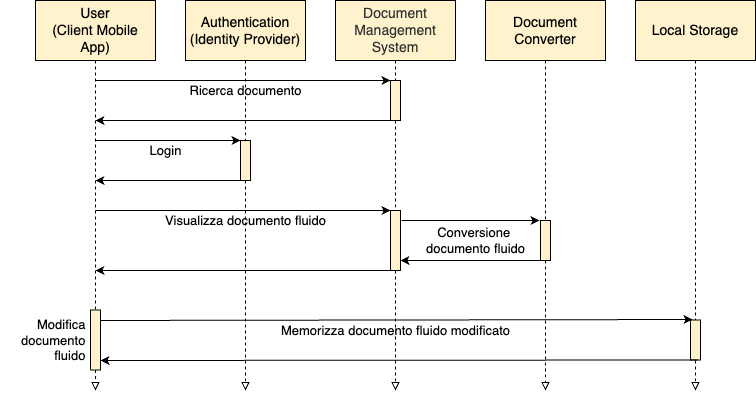
\includegraphics[width=1\textwidth]{img/tesi-2-Use-case2.drawio.png}
\caption{UML - Diagramma di sequenza: scenario di modifica di un nuovo documento "fluido".}
\end{figure}

\subsection{Requisiti Non Funzionali/Tecnologici}
\begin{itemize}
    \item \textbf{T1} - Applicazione nativa Android e iOS, sfruttando Kotlin Multiplatform Mobile (KMM).
    \item \textbf{T2} - Continuous Integration e Continuous Delivery
    \begin{itemize}
        \item \textbf{T2.1} - Analisi statica del codice (SAST\footnote{Static Application Security Testing}).
        \item \textbf{T2.2} - Unit testing, code coverage e UI testing.
        \item \textbf{T2.3} - Rilascio automatico nei relativi store delle piattaforme scelte (Google Play per Android e App Store per iOS).
    \end{itemize}
\end{itemize}

\begin{figure}[H]
\centering
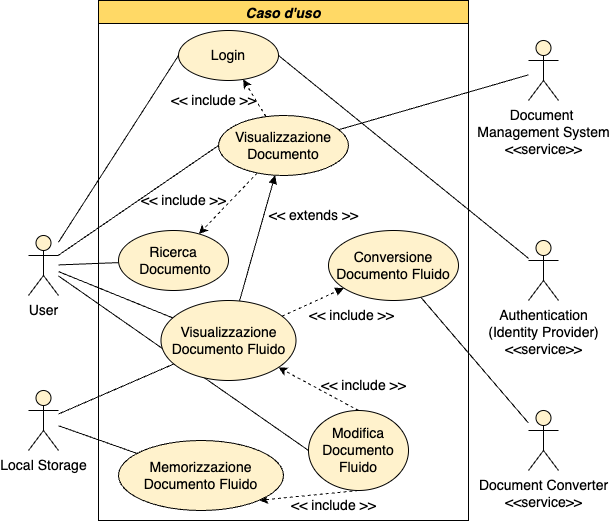
\includegraphics[width=1\textwidth]{img/tesi-1-Use-case.drawio.png}
\caption{UML - Diagramma dei casi d'uso: funzioni/servizi offerti dal sistema Ebook App PoC.}
\end{figure}

\section{Progettazione}
In questa sezione viene descritta la fase di progettazione del sistema, le cui attività principali consistono nella ($i$) modellazione del dominio, nella progettazione della architettura ($ii$) e ($iii$) nella progettazione dell'interfaccia grafica tramite mockup.

\subsection{Modellazione Dominio}
In base ai casi d'uso e ai requisiti della applicazione individuati in fase di analisi è possibile identificare tre contesti all'interno del dominio:

\begin{itemize}
    \item \textit{Reader} (Core) - Contesto principale del progetto. Racchiude tutti gli aspetti con maggiore valore per l'utente riguardanti la lettura e la personalizzazione dei contenuti digitali. 
    \item \textit{Sisred} - Rappresenta il contesto della sorgente dei contenuti digitali Maggioli (Sistema Redazionale\cite{amslaurea23043}). In questo contesto non esistono i concetti di \textit{favorite}, \textit{highlight}, \textit{bookmark} e \textit{progression} mentre è condiviso il concetto di libro e utente.
    \item \textit{User} - Contesto che definisce tutti gli aspetti a riguardo degli utenti. In questo contesto esiste il solo concetto di utente, il quale è condiviso con gli altri contesti.
\end{itemize}

\begin{figure}[H]
\centering
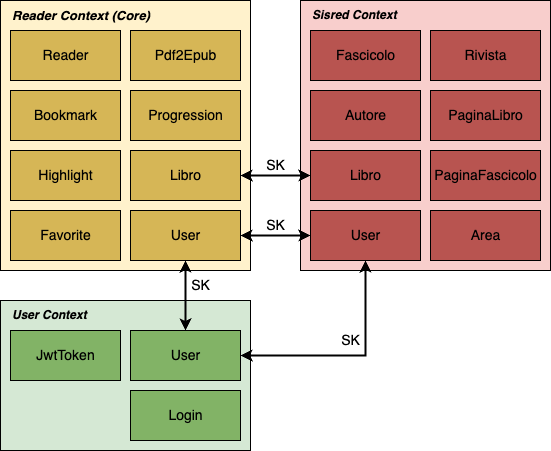
\includegraphics[width=0.7\textwidth]{img/tesi-20-app-domain.drawio.png}
\caption{Context Map: panoramica globale dei contesti del progetto e delle relazioni che intercorrono tra di essi.}
\end{figure}

\begin{figure}[H]
\centering
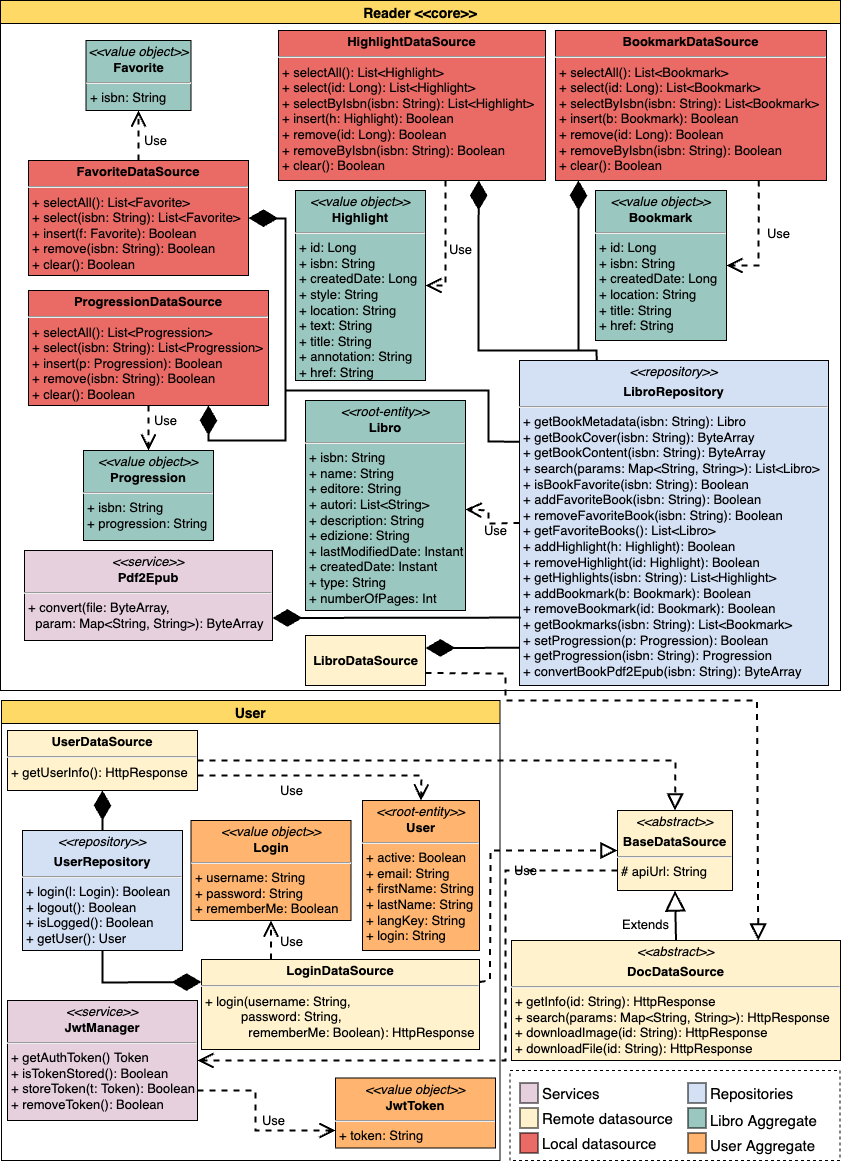
\includegraphics[width=0.9\textwidth]{img/tesi-25-ddd.drawio.png}
\caption{UML - Diagramma delle classi: Reader Core Domain e User Subdomain.}
\label{fig:5.4}
\end{figure}

Tra i contesti definiti esistono delle relazioni di tipo \textit{Shared Kernel}\cite{evans_domain-driven_2004} (SK) con l'obiettivo di evitare duplicazioni e semplificare l'integrazione. Relazioni di questo tipo consistono nella condivisione di un sottoinsieme del dominio modellato, che corrisponde tipicamente al dominio core. Un esempio di relazione SK è l'utilizzo di codice o schemi DB condivisi\footnote{\url{https://github.com/ddd-crew/context-mapping}}.\\
Per la modellazione del dominio si fa uso dei seguenti concetti\cite{evans_domain-driven_2004}:
\begin{itemize}
    \item \textit{Entity} - Oggetto definito dalla sua identità e non dai suoi attributi. Ogni libro è univoco, identificato da uno specifico codice, chiamato ISBN\footnote{International Standard Book Number}.
    \item \textit{Value Object} - Al contrario delle entità, questi oggetti sono definiti dai loro attributi e non hanno una identità concettuale ma servono a descrivere alcune caratteristiche di un oggetto. Un esempio è il segnalibro: ciò che è rilevante è la pagina del libro che esso referenzia e non la sua identità.
    \item \textit{Aggregate} - Insieme di oggetti legati da una entità padre chiamata \textit{Root} (radice di aggregazione). L'aggregato composto da \textit{Bookmark}, \textit{Highlight}, \textit{Progression}, \textit{Favorite} ha come radice l'entità \textit{Libro}.
    \item \textit{Service} - Operazione che non appartiene logicamente a nessun oggetto. In questo caso la conversione di formato non appartiene alla sola entità libro ma appartiene invece a qualsiasi documento che è possibile convertire.
    \item \textit{Repository} - Oggetto per il recupero di altri oggetti di dominio e per la gestione del loro ciclo di vita. Le entità \textit{User} e \textit{Libro} sono esempi di oggetti di dominio che necessitano di un repository. Permette di disaccoppiare applicazione e domain design dalle specifiche tecnologie/strategie di persistenza come multipli database e datasource (locali e/o remoti).
\end{itemize}

L'architettura progettata per la applicazione segue la struttura \textit{Clean Architecture}\cite{Martin17} ed è composta da tre strati. Il primo strato (\textit{Data Layer}) consiste negli aggregati di dominio sopra descritti ed è responsabile per il recupero e il mantenimento dei dati su differenti sorgenti. Il secondo strato (\textit{Domain Layer}) facilità la comunicazione tra i differenti repository: qui si trovano tutti i casi d'uso del sistema che gestiscono il flusso dei dati provenienti o diretti verso il primo strato. Il terzo ed ultimo strato (\textit{View Layer}) si occupa della interfaccia grafica mostrando i dati e gestendo gli eventi provenienti dall'utente o dal sistema.

\begin{figure}[H]
\centering
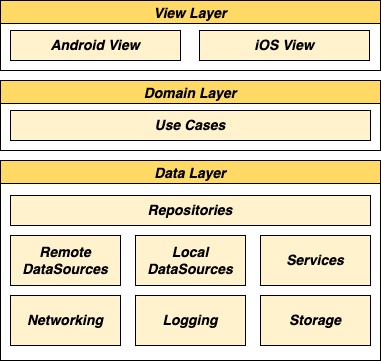
\includegraphics[width=0.55\textwidth]{img/tesi-2-Page-18.drawio.png}
\caption{Clean Architecture in MaggioliEbook.}
\end{figure}

\subsection{Progettazione UX/UI}

L'interfaccia grafica della applicazione è stata progettata tramite l'utilizzo di mockup digitali realizzati con il tool grafico open source Drawio\footnote{\url{https://github.com/jgraph/drawio}}.\\
Considerando l'utilizzo tipico di una applicazione della stessa tipologia di quella che deve essere realizzata, sono stati utilizzati alcuni standard de-facto come ad esempio il menu laterale a scomparsa (schermata 4), icona "hamburger" per l'apertura del menu (schermata 3), elenco di elementi con scroll infinito verticale (schermata 2-5) e barra di ricerca nella parte alta con icona "lente di ingrandimento" (schermata 2-5).\\
Per ottenere la validazione dei mockup da parte del committente sono state necessarie due iterazioni del processo di progettazione UX/UI. L'interfaccia utente desiderata deve soddisfare alcuni vincoli caratteristici del brand Maggioli: ad esempio l' utilizzo del colore blu \#00379E come colore primario, l'utilizzo del font Karla\footnote{\url{https://github.com/googlefonts/karla}} e la presenza del logo Maggioli. Le schermate necessarie sono quindi: \textit{Reader}, responsabile della visualizzazione del contenuto digitale in formato EPUB; \textit{Login}, schermata iniziale responsabile alla autenticazione dell'utente; \textit{Home}, schermata principale responsabile alla visualizzazione dei contenuti digitali a cui l'utente è autorizzato ad accedere; \textit{Preferiti}, responsabile alla visualizzazione dei contenuti digitali preferiti dall'utente; \textit{Impostazioni}, responsabile alla visualizzazione e modifica delle impostazioni; \textit{About}, responsabile alla visualizzazione di informazioni generali come versione della applicazione, autore e copyright.

\begin{figure}[H]
\centering
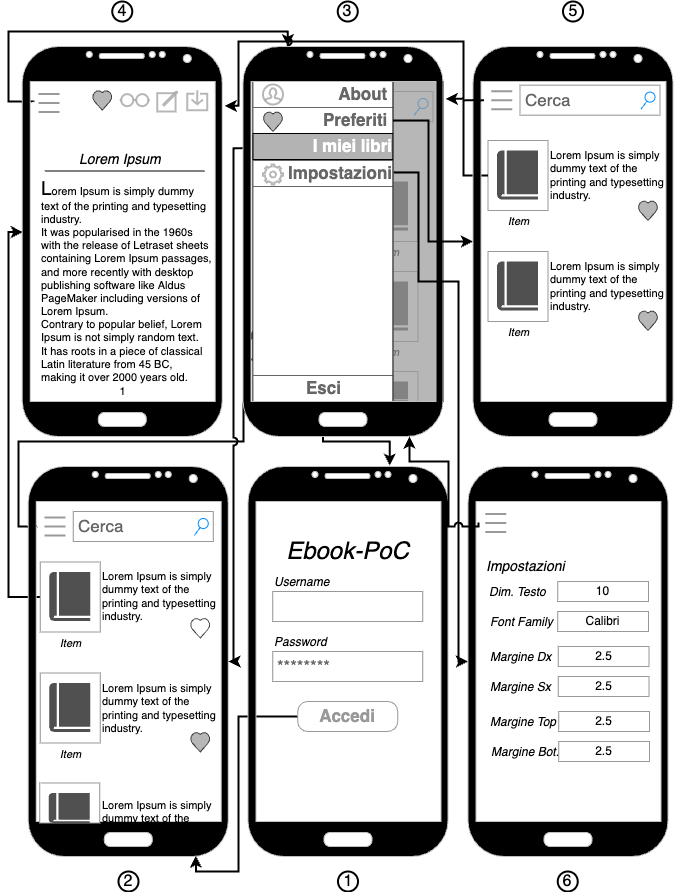
\includegraphics[width=1\textwidth]{img/tesi-14-mockup1.drawio.png}
\caption{Alcuni dei mockup realizzati per la progettazione e la validazione della UX/UI (v1)}
\end{figure}

\begin{figure}[H]
\centering
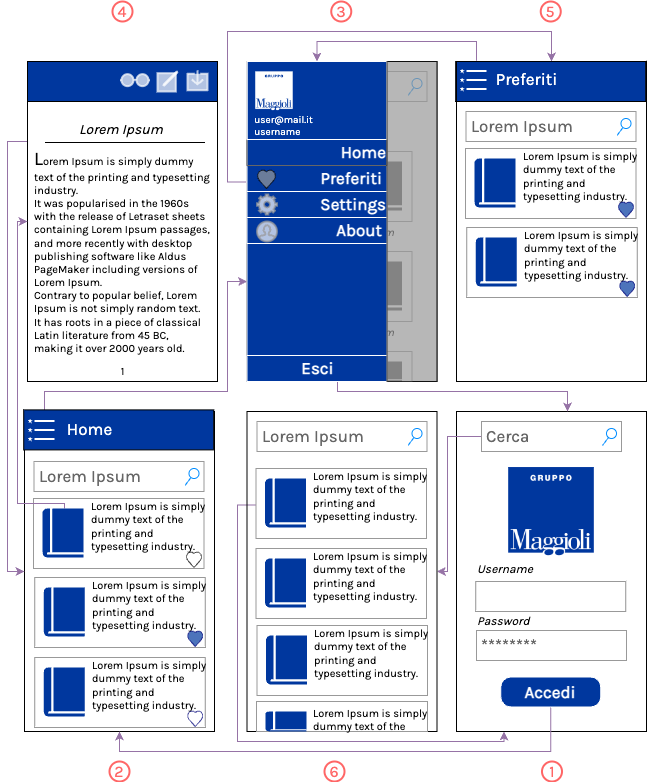
\includegraphics[width=0.95\textwidth]{img/tesi-23-mockupv2.drawio.png}
\caption{Modifiche apportate ai mockup per ottenere la validazione della UX/UI (v2)}
\end{figure}

\section{Implementazione}
La fase di implementazione consiste nello sviluppo della applicazione secondo il paradigma Kotlin Multiplatform: sono presenti infatti un unico core, chiamato \textit{shared} ($i$), che definisce la logica condivisa della applicazione e due differenti implementazioni per l'interfaccia utente, chiamate rispettivamente \textit{androidMaggioliEbookApp} ($ii$) e \textit{iosMaggioliEbookApp} ($iii$).

\subsection{Ricerca Librerie}
La prima attività svolta nella fase di implementazione è stata la ricerca delle librerie, la quale ha permesso di individuare le seguenti librerie, suddivise per modulo di appartenenza:
\begin{itemize}
    \item \textit{Shared}
    \begin{itemize}
        \item \textit{Ktor} - Framework asincrono per lo sviluppo di microservizi e applicazioni web. Nel progetto Ktor è utilizzato per la parte di networking come client HTTP.
        \item \textit{Kotlinx-Serialization} - Libreria multiplatform per la serializzazione dei dati.
        \item \textit{Kotlinx-Datetime} - Libreria multiplatform per la gestione delle date e del tempo.
        \item \textit{Kvault}\footnote{\url{https://github.com/Liftric/KVault}} - Libreria multiplatform per la persistenza dei dati sicura in formato chiave-valore. Tramite una unica API si comporta come wrapper di Keychain, nel caso iOS, e SharedPreferences nel caso Android.
        \item \textit{Koin}\footnote{\url{https://github.com/InsertKoinIO/koin}} - Dependency Injection framework multiplatform.
        \item \textit{Napier}\footnote{\url{https://github.com/AAkira/Napier}} - Logging framework multiplatform.
        \item \textit{SqlDelight}\footnote{\url{https://github.com/cashapp/sqldelight}} - Libreria multiplatform per la persistenza dei dati tramite database relazionale locale.
    \end{itemize}
    \item \textit{Android}
    \begin{itemize}
    \item \textit{Readium} (Kotlin-toolkit)\footnote{\url{https://github.com/readium/kotlin-toolkit}} - Libreria per la manipolazione e visualizzazione di contenuti editoriali digitali. Implementazione specifica per la piattaforma Android. 
    \end{itemize}
    \item \textit{iOS}
    \begin{itemize}
    \item \textit{Readium} (Swift-toolkit)\footnote{\url{https://github.com/readium/swift-toolkit}} - Libreria per la manipolazione e visualizzazione di contenuti editoriali digitali. Implementazione specifica per la piattaforma iOS. 
    \item \textit{KMPNativeCoroutines}\footnote{\url{https://github.com/rickclephas/KMP-NativeCoroutines}} - Libreria che permette l'utilizzo delle coroutine Kotlin in Swift in applicazioni Kotlin Multiplatform.
    \end{itemize}
\end{itemize}
Per ognuna delle librerie del modulo \textit{Shared} esistono valide alternative, dimostrando che l'ecosistema Kotlin Multiplatform è in continua espansione\footnote{\url{https://github.com/terrakok/kmm-awesome}}.

\subsection{Readium}
Le uniche due librerie individuate che da documentazione sono in grado di rispettare i requisiti di gestione, manipolazione e visualizzazione dei contenuti digitali in formato EPUB sono \textit{Readium}\footnote{\url{https://github.com/readium}} e \textit{FolioReader}\footnote{\url{https://github.com/FolioReader}}.\\
Entrambe le librerie forniscono le stesse identiche funzionalità ma è stata scelta \textit{Readium} come libreria per la applicazione per le seguenti motivazioni:
\begin{itemize}
    \item Non è stato possibile testare la libreria \textit{FolioReader} a causa di errori al suo interno in fase di compilazione della applicazione di test realizzata.
    \item Per la libreria \textit{Readium} l'ultima commit per la versione Android risale al 05/09/2022 e l'ultimo rilascio risale al 22/04/2022, mentre per la libreria \textit{FolioReader} l'ultima commit per la versione Android risale al 09/01/2020 e l'ultimo rilascio risale al 11/01/2019. Lo stesso confronto è valido per la versione iOS.\footnote{Dati al 06/09/2022 provenienti dai relativi repository GitHub}
    \item La libreria \textit{Readium} è scritta con in Kotlin mentre \textit{FolioReader} è scritta in Java.
\end{itemize}
La necessità di un tool open-source, robusto e performante per la manipolazione e la lettura di formati editoriali digitali è alla base del progetto Readium. Essa infatti consiste in un insieme di toolkit per diversi formati (come epub, audiolibri e libri image-based) e diverse piattaforme (Android, iOS, Desktop e Web).\\
L'architettura della libreria \textit{Readium} è composta da quattro moduli principali:
\begin{itemize}
    \item \textit{Publication Server} - Fornisce le pubblicazioni tramite un server locale HTTPS.
    \item \textit{Streamer} - Modulo composto dai seguenti due sottomoduli:
    \begin{itemize}
        \item \textit{Parser} - Responsabile del parsing delle pubblicazioni e della loro esposizione utilizzando un modello in-memory.
        \item \textit{Fetcher} - Si occupa di ottenere i contenuti delle pubblicazioni e della loro manipolazione (in particolare injection di CSS e Javascript nelle risorse HTML).
    \end{itemize}
    \item \textit{Navigator} - Utile alla navigazione delle risorse di una pubblicazione secondo diverse strategie basate sulla natura della pubblicazione (ebook, audiolibri, ...). Interagisce con il modulo \textit{Streamer} per utilizzare il modello in-memory o per ottenere manifesto JSON attraverso il modello condiviso (\textit{Shared}).
\end{itemize}
\begin{figure}[H]
\centering
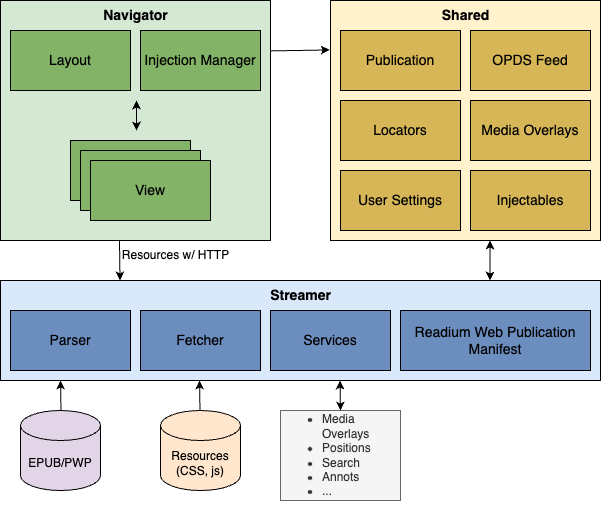
\includegraphics[width=0.7\textwidth]{img/tesi-22-readiumarch.drawio.png}
\caption{Architettura libreria Readium}
\label{readiumarch}
\end{figure}

\subsection{Shared}
Come anticipato nel capitolo \ref{ch:ch3} la parte condivisa della applicazione racchiude tutta o una sottoparte della business logic, compresi quindi aspetti "infrastrutturali" specifici della piattaforma target come ad esempio logging, persistenza dei dati e networking. E' infatti in questo modulo che si trova l'implementazione della logica applicativa sviluppata nel rispetto delle specifiche definite in fase di progettazione (figura \ref{fig:5.4}).\\
Lo schema del database locale è definito utilizzando appositi file, in formato \textit{.sq}, uno per ognuna delle entità che necessita di persistenza: \textit{Highlight}, \textit{Favorite}, \textit{Progression} e \textit{Bookmark}. Tramite il task \textit{generateSqlDelightInterface} fornito dal plugin gradle SqlDelight è possibile generare le relative implementazioni dell'interfaccia \textit{MaggioliEbookDB}, anch'essa autogenerata dal plugin. 

\begin{figure}[H]
\centering
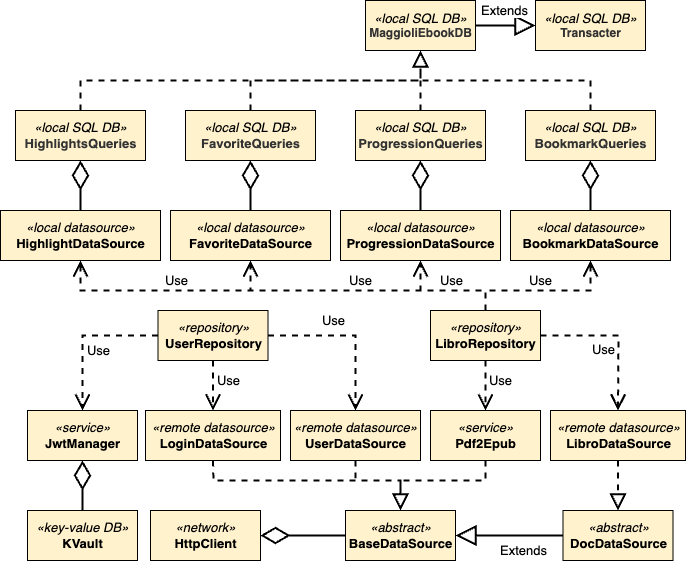
\includegraphics[width=1\textwidth]{img/tesi-26-shareduml.drawio.png}
\caption{UML - Diagramma delle classi: Implementazioni data source (persistenza dati e networking)}
\end{figure}

\begin{listing}[H]
\inputminted{sql}{code/5-sqldelight}
\caption{Esempio di definizione schema \textit{Bookmark} tramite sintassi SqlDelight}
\end{listing}

\begin{listing}[H]
\inputminted{kotlin}{code/5-sqldelight1}
\caption{Implementazione autogenerata tramite il plugin gradle SqlDelight della precedente definizione dello schema per l'entità \textit{Bookmark}}
\end{listing}

Tipicamente le librerie per applicazioni sviluppate con Kotlin Multiplatform possono essere utilizzate direttamente dal codice condiviso, come ad esempio KVault, lasciando al compilatore Kotlin il compito di scegliere la giusta implementazione per la piattaforma target durante la fase di compilazione. In altri casi è necessario invece utilizzare il meccanismo \textit{expect/actual} (discusso nel capitolo \ref{ch:ch3}) per definire il comportamento atteso e fornire una implementazione specifica per la piattaforma target.\\
Tale meccanismo è stato utilizzato nello sviluppo della applicazione per poter effettuare dependency injection tramite la libreria Koin dei componenti riguardanti la persistenza dei dati (Kvault e SqlDelight) e l'esecuzione asincrona (CoroutineDispatcher).

\begin{figure}[H]
\centering
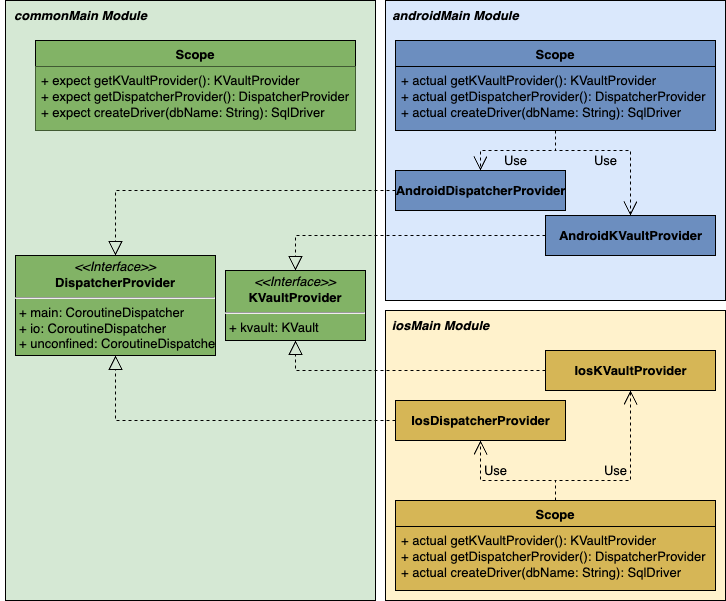
\includegraphics[width=0.9\textwidth]{img/tesi-21-expectactual.drawio.png}
\caption{Strategia \textit{Expect/Actual} adottata per l'implementazione dei servizi infrastrutturali specifici delle piattaforme, persistenza e concorrenza, sfruttando la tecnica \textit{dependency injection}}
\end{figure}

Ogni dipendenza che deve essere iniettata viene inserita all'interno di uno o più moduli, i quali vengono utilizzati da Koin per inizializzare tutto il contesto applicativo. Le dipendenze possono essere principalmente di due tipi:
\begin{itemize}
    \item \textit{Factory} - Ogni volta che la dipendenza viene iniettata ne viene creata una nuova istanza (paragonabile al design pattern Factory Method\footnote{\url{https://en.wikipedia.org/wiki/Factory_method_pattern}}).
    \item \textit{Single} - In tutto il contesto applicativo esiste una sola istanza della dipendenza iniettata (paragonabile al design pattern Singleton\footnote{\url{https://en.wikipedia.org/wiki/Singleton_pattern}}).
\end{itemize}

\begin{listing}[H]
\inputminted{kotlin}{code/5-koin}
\caption{Configurazione Dependency Injection: definizione dei moduli Koin e inizializzazione del contesto applicativo}
\end{listing}

\subsection{androidMaggioliEbookApp}
L'applicazione sviluppata per la piattaforma Android implementa sia lo strato della visualizzazione dei dati utilizzando la business logic fornita dal modulo \textit{Shared} che la logica del \textit{Reader}, lettore dei contenuti digitali realizzato tramite il toolkit Kotlin della libreria \textit{Readium}.
\subsubsection{Single-Activity Architecture}
L'architettura scelta per l'implementazione della applicazione Android è basata su sole due activity:
\begin{itemize}
    \item \textit{MainActivity} - Unica activity principale della applicazione.
    \item \textit{ReaderActivity} - Activity secondaria, utilizzata sia per l'interazione che la gestione del lettore di contenuti digitali.
\end{itemize}
Questa tipologia di architettura permette di avere una singola activity che svolge la funzione di "big container" per tutti i fragment che rappresentano le varie schermate della applicazione.

\begin{figure}[H]
\centering
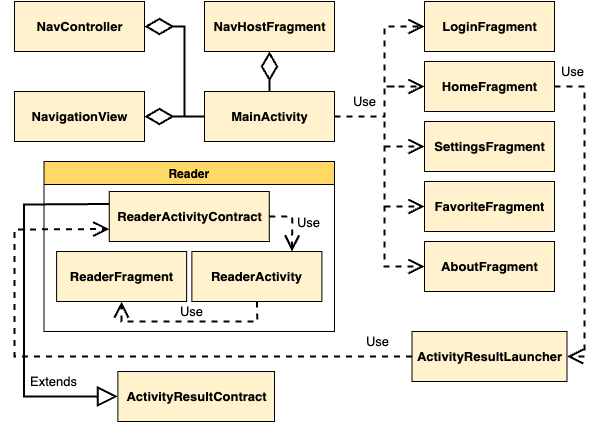
\includegraphics[width=0.7\textwidth]{img/tesi-27-singleactivity.drawio.png}
\caption{UML - Diagramma delle classi: architettura Single-Activity}
\label{fig:5.10}
\end{figure}

La navigazione all'interno della applicazione è gestita tramite la combinazione dei seguenti componenti:
\begin{itemize}
    \item \textit{NavController} - Componente necessario per la gestione delle transizioni da un un fragment all'altro. Quando inizializzato richiede la presenza di un grafo di navigazione tra le risorse XML: tale grafo contiene tutti i fragment che possono essere visualizzati e le possibili transizioni tra di essi.
    \item \textit{NavHostFragment} - Rappresenta il contenitore del fragment in cui ci si trova. Ogni transizione nel grafo corrisponde alla sostituzione del fragment visualizzato con quello di destinazione (sempre che la transizione sia ammessa dal grafo).
    \item \textit{NavigationView} - Permette la visualizzazione del menu dove si trovano i possibili fragment raggiungibili da quello in cui l'utente si trova attualmente. Nel caso della applicazione sviluppata in questo componente si trova il menu laterale con tutte le schermate indicate in fase di progettazione (\textit{Home}, \textit{Settings}, \textit{About} e \textit{Preferiti}).
\end{itemize}

\begin{figure}[H]
\centering
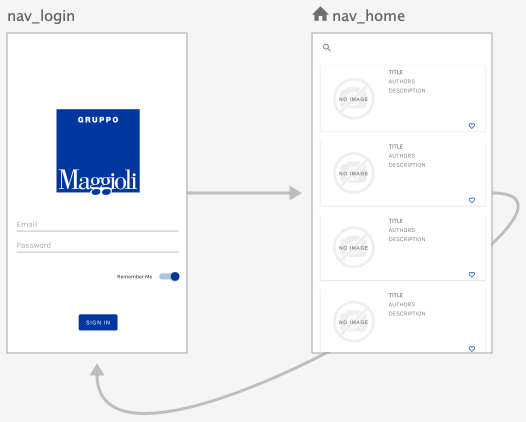
\includegraphics[width=0.7\textwidth]{img/Screenshot 2022-09-20 at 08.26.21.png}
\caption{Screenshot di una sottoparte del navigation graph (renderizzato automaticamente tramite l'IDE Android Studio)}
\label{fig:5.11}
\end{figure}

Come indicato nella figura \ref{fig:5.11} la schermata principale (\textit{Home}) rappresenta la destinazione iniziale del grafo, ovvero la prima schermata che viene visualizzata dalla applicazione. L'autenticazione dell'utente è gestita tramite la navigazione condizionale\footnote{\url{https://developer.android.com/guide/navigation/navigation-conditional}}. Prima di creare la vista del fragment viene effettuato un controllo sulla autenticazione dell'utente: se l'utente non è autenticato viene effettuata una transizione al fragment \textit{Login} per permettere all'utente di autenticarsi e procedere all'utilizzo della applicazione. E' fondamentale in questo scenario ripulire lo stack di navigazione per evitare che l'utente possa tornare indietro alla schermata precedente, ovvero la schermata principale, senza effettuare l'autenticazione.\\

\subsubsection{Paging}
Un altro aspetto importante della architettura è il meccanismo utilizzato sia dalla schermata principale che da quella dei preferiti per mostrare i dati all'utente. Il backend utilizzato fornisce i dati tramite paginazione: in questo modo è possibile indicare in una richiesta la dimensione delle pagine, ovvero quanti elementi devono essere restituiti al massimo in una pagina, e la pagina desiderata. Per poter caricare tali dati dinamicamente in una \textit{RecyclerView}\footnote{\url{https://developer.android.com/reference/kotlin/androidx/recyclerview/widget/RecyclerView}} in modo che l'utente possa effettuare lo scroll illimitato nella schermata si utilizza la libreria \textit{Paging}\footnote{\url{https://developer.android.com/topic/libraries/architecture/paging/v3-overview}} fornita da Android.

\begin{figure}[H]
\centering
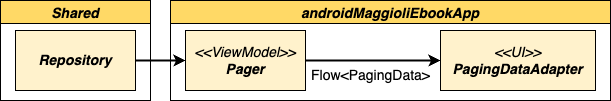
\includegraphics[width=0.75\textwidth]{img/tesi-2-Page-11.drawio.png}
\caption{Flusso generico dei dati dalla sorgente alla UI tramite l'utilizzo della libreria Paging}
\label{paging}
\end{figure}

I componenti fondamentali della libreria \textit{Paging} sono:
\begin{itemize}
    \item \textit{Pager} - Punto di ingresso principale della libreria con il compito di ottenere nuovi dati quando necessario, ovvero quando l'utente ha scrollato nella schermata fino ad uno specifico punto. Richiede la configurazione di alcuni parametri come la dimensione della pagina, la pagina iniziale e la direzione della paginazione. 
    \item \textit{PagingSource} - Sorgente dei dati paginati. Componente interrogato dal \textit{Pager} ogni volta che sono necessari nuovi dati.
    \item \textit{PagingDataAdapter} - Componente fondamentale per la rappresentazione di dati paginati in una \textit{RecyclerView}.
\end{itemize}

\begin{figure}[H]
\centering
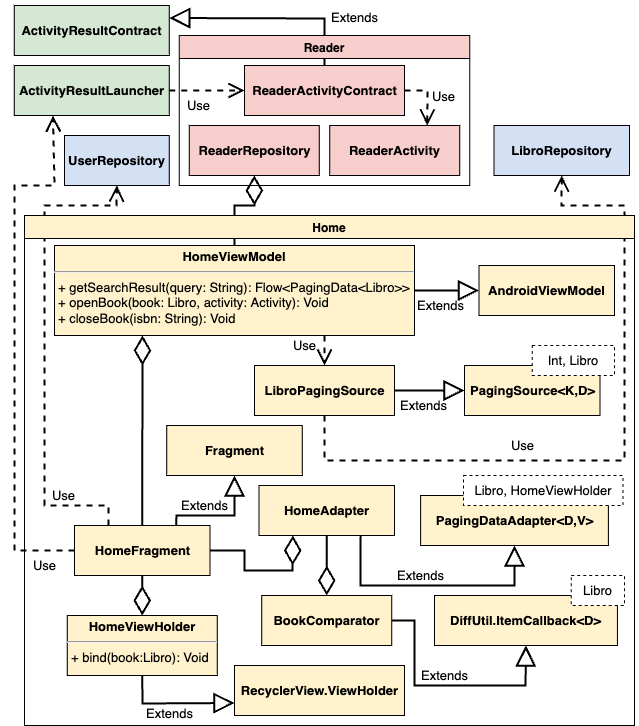
\includegraphics[width=0.7\textwidth]{img/tesi-24-androidviewuml.drawio.png}
\caption{UML - Diagramma delle classi: Paginazione dati nella schermata principale}
\label{paging2}
\end{figure}

\subsubsection{Reader}
Il lettore dei documenti digitali in formato EPUB rappresenta la funzionalità core della applicazione sviluppata. Nel caso della interfaccia grafica android il lettore riceve il contenuto da visualizzare del documento selezionato dall'utente e lo mostra in un fragment basato sul componente \textit{Navigator} (figura \ref{readiumarch}). Questo componente della libreria Readium fornisce tutte le funzionalità necessarie per gestire la navigazione dei documenti e gli eventi relativi al comportamento dell'utente come scorrimento pagine e selezione testo. \\
I principali componenti del reader sono:
\begin{itemize}
    \item \textit{ReaderActivity} - Unica activity presente nella applicazione oltre a quella principale (Single Activity Architecture), utilizzata sia per l’interazione che la gestione del lettore di contenuti digitali.
    \item \textit{EpubReaderFragment} - Componente che si occupa effettivamente di mostrare il contenuto del documento all'utente.
    \item \textit{DecorationListener} - Permette la gestione grafica delle annotazioni come evidenziazioni e sottolineature, le quali sono aggiunte alla vista del fragment tramite l'utilizzo di Jetpack Compose.
\end{itemize}

\begin{figure}[H]
\centering
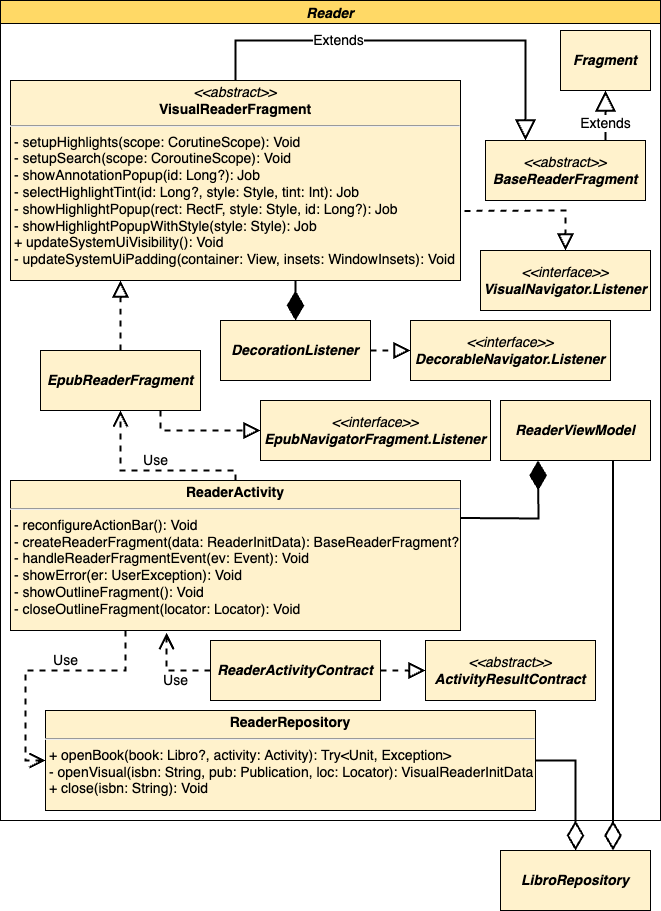
\includegraphics[width=0.75\textwidth]{img/tesi-2-Page-16.drawio.png}
\caption{UML - Diagramma delle classi: Reader}
\label{reader}
\end{figure}

\subsubsection{Screenshots}

\begin{multicols}{3}
            \begin{figure}[H]
                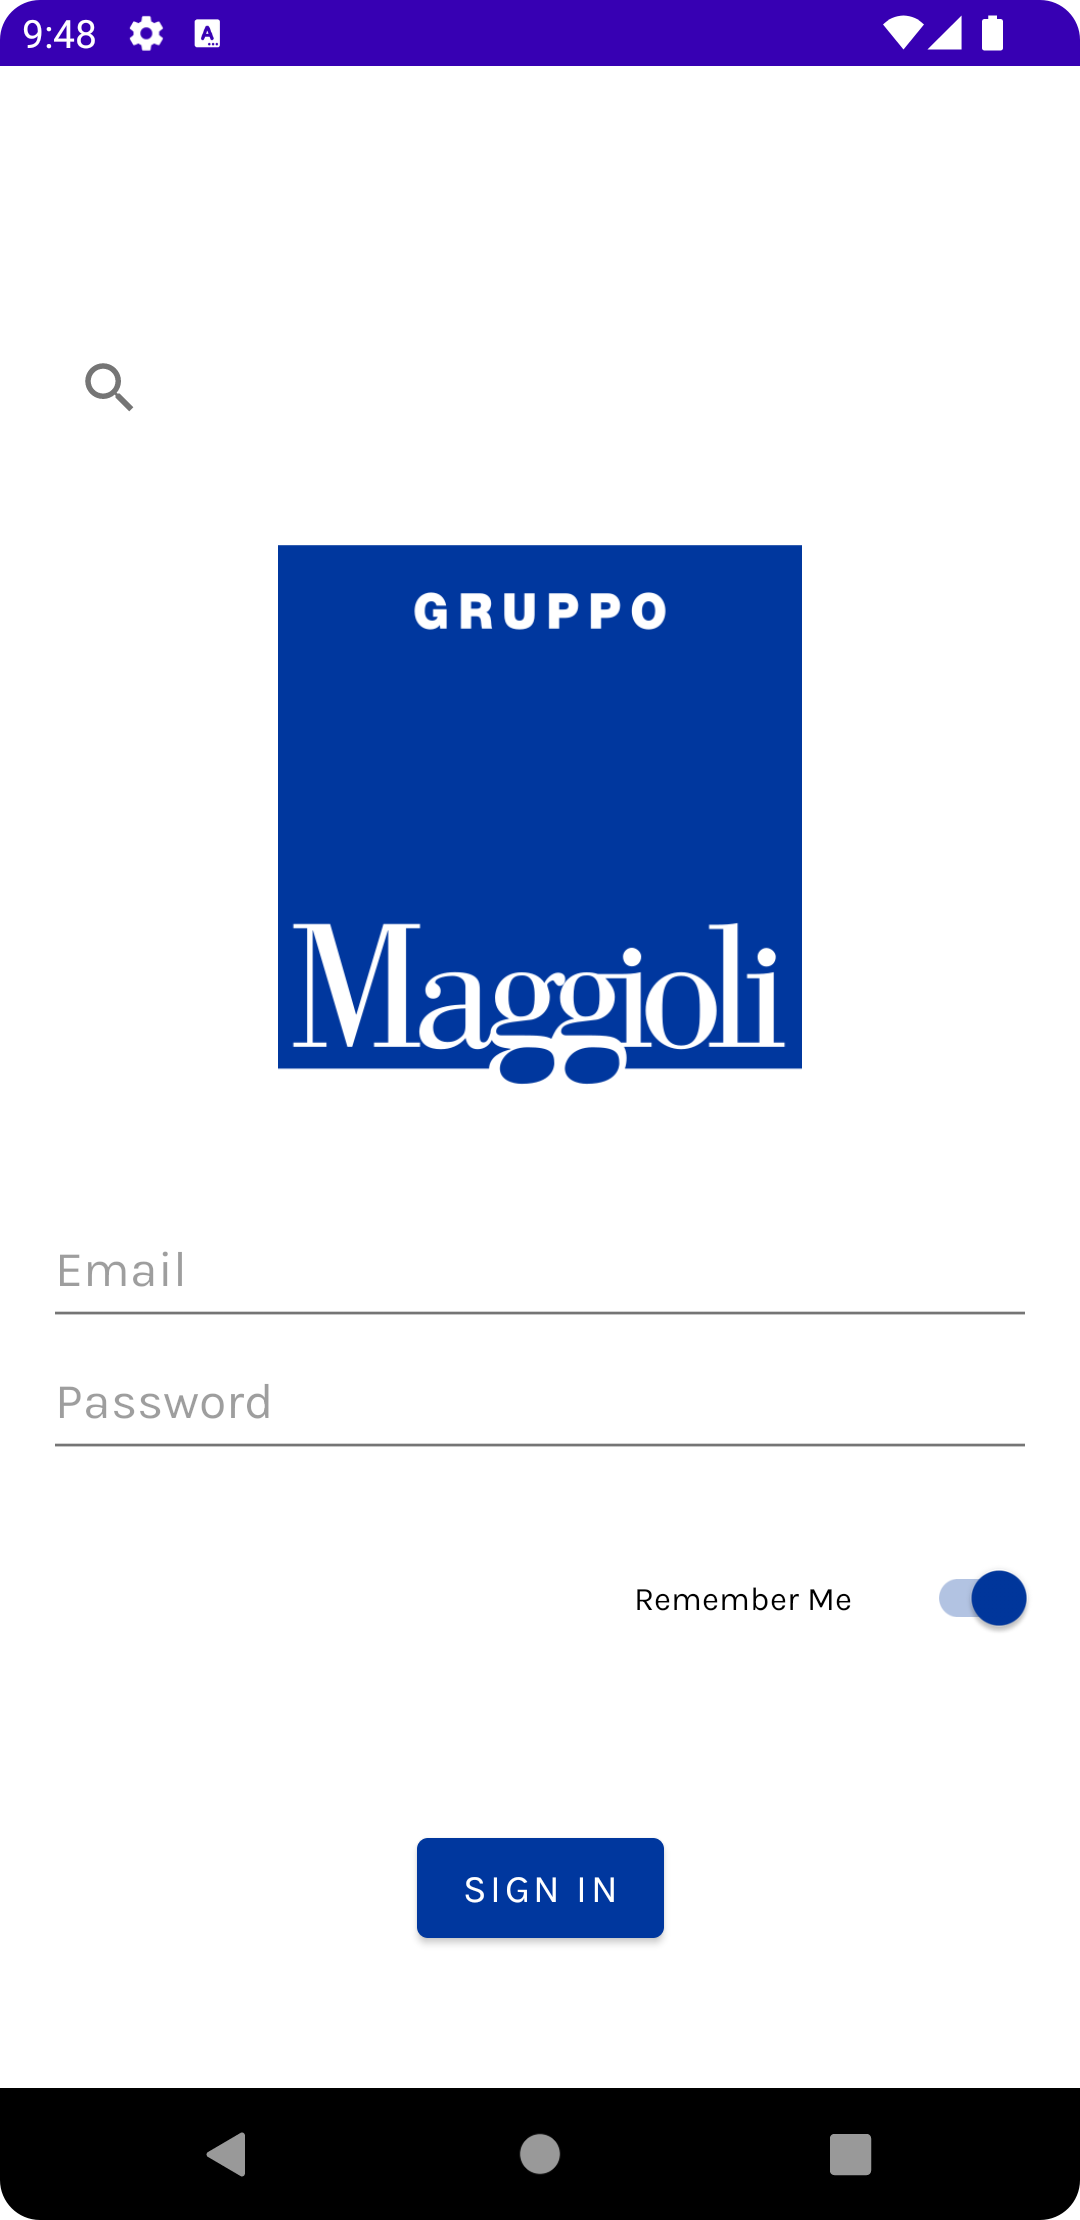
\includegraphics[width=0.21\textwidth]{img/login.png}
                \caption{Schermata di login degli utenti abbonati}
                \label{login}
            \end{figure}

            \begin{figure}[H]
                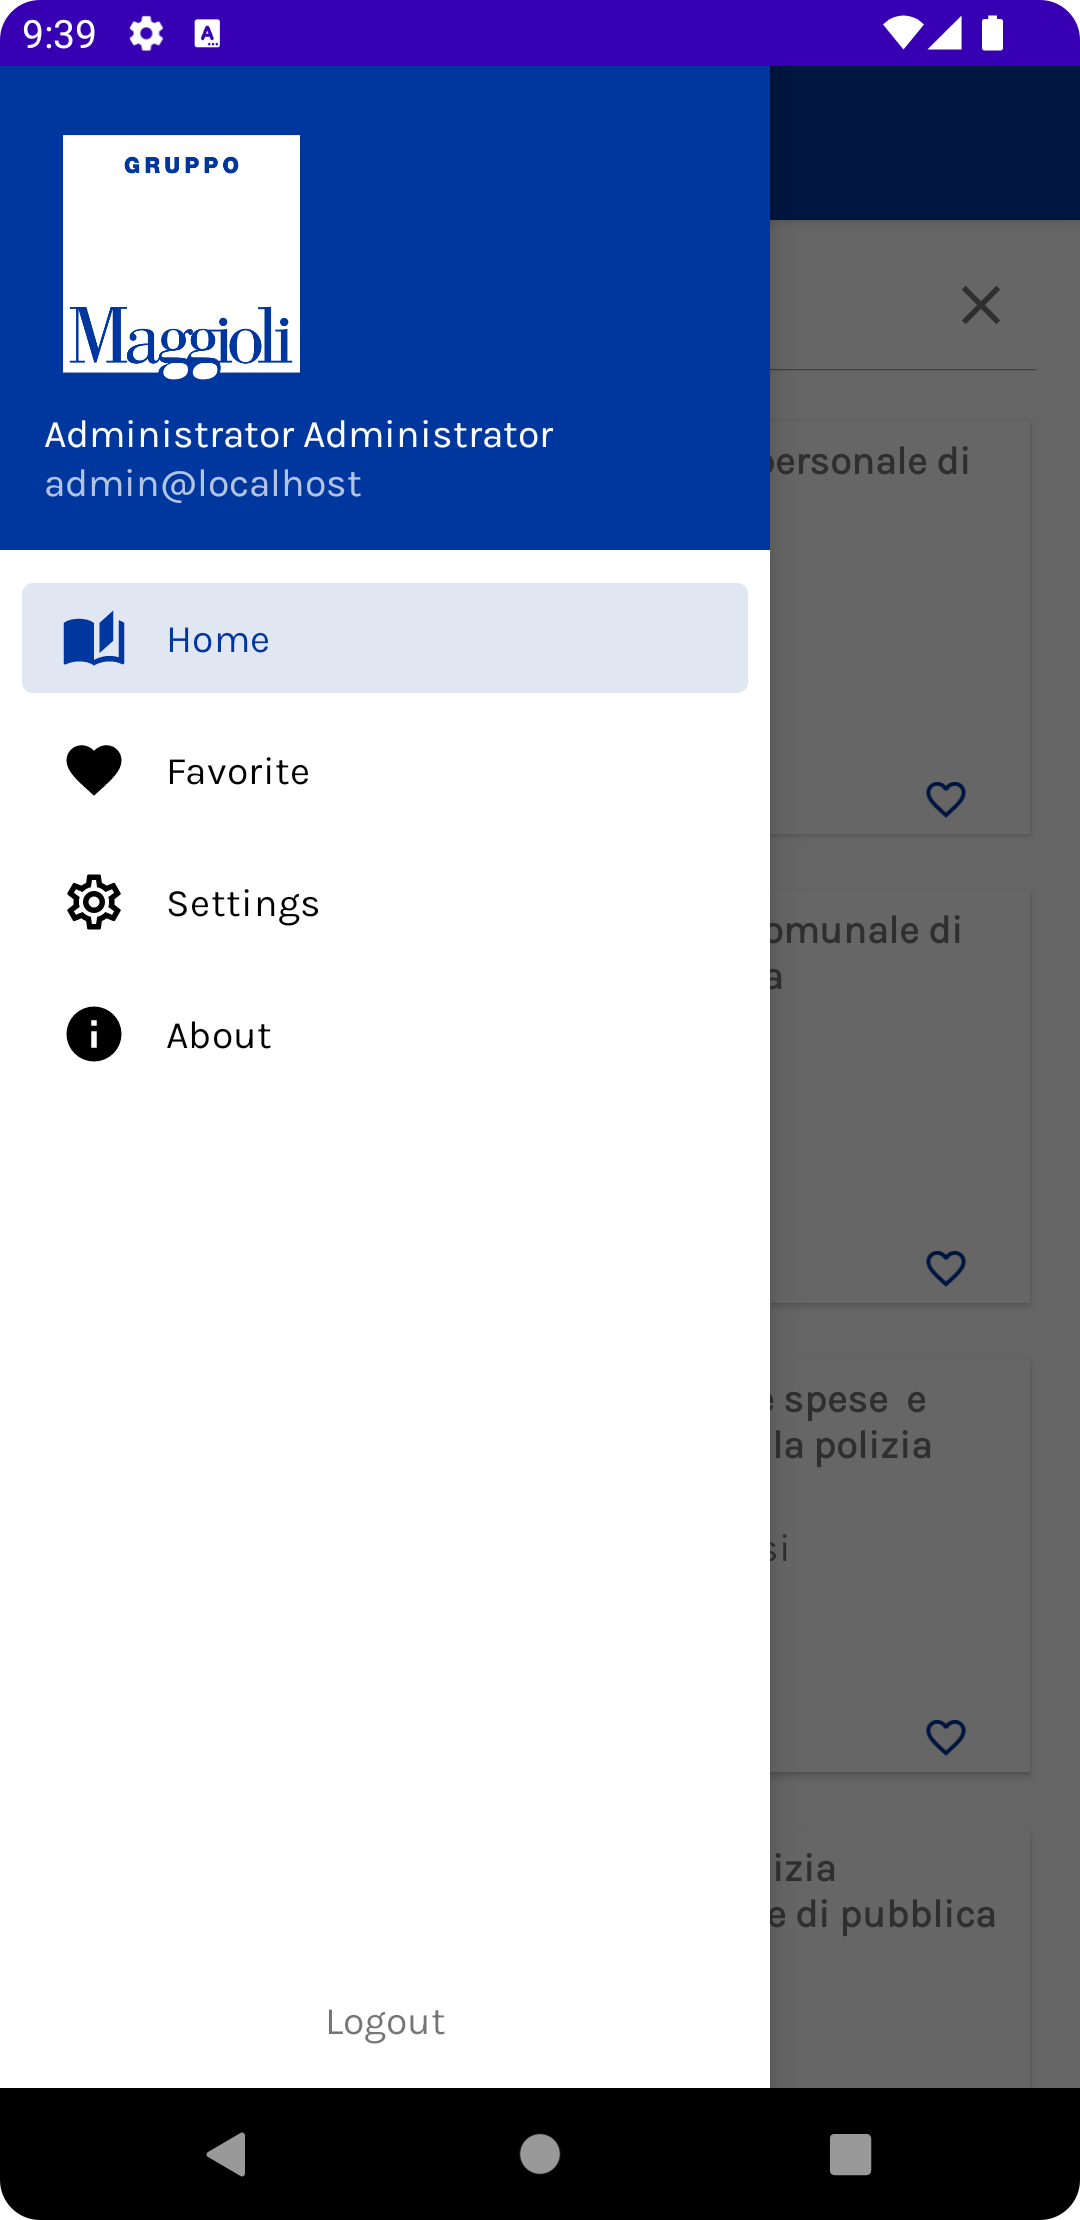
\includegraphics[width=0.21\textwidth]{img/sidenav.png}
                \caption{Menu laterale per la navigazione all'interno della applicazione}
                \label{sidenav}
            \end{figure}
            
            \begin{figure}[H]
                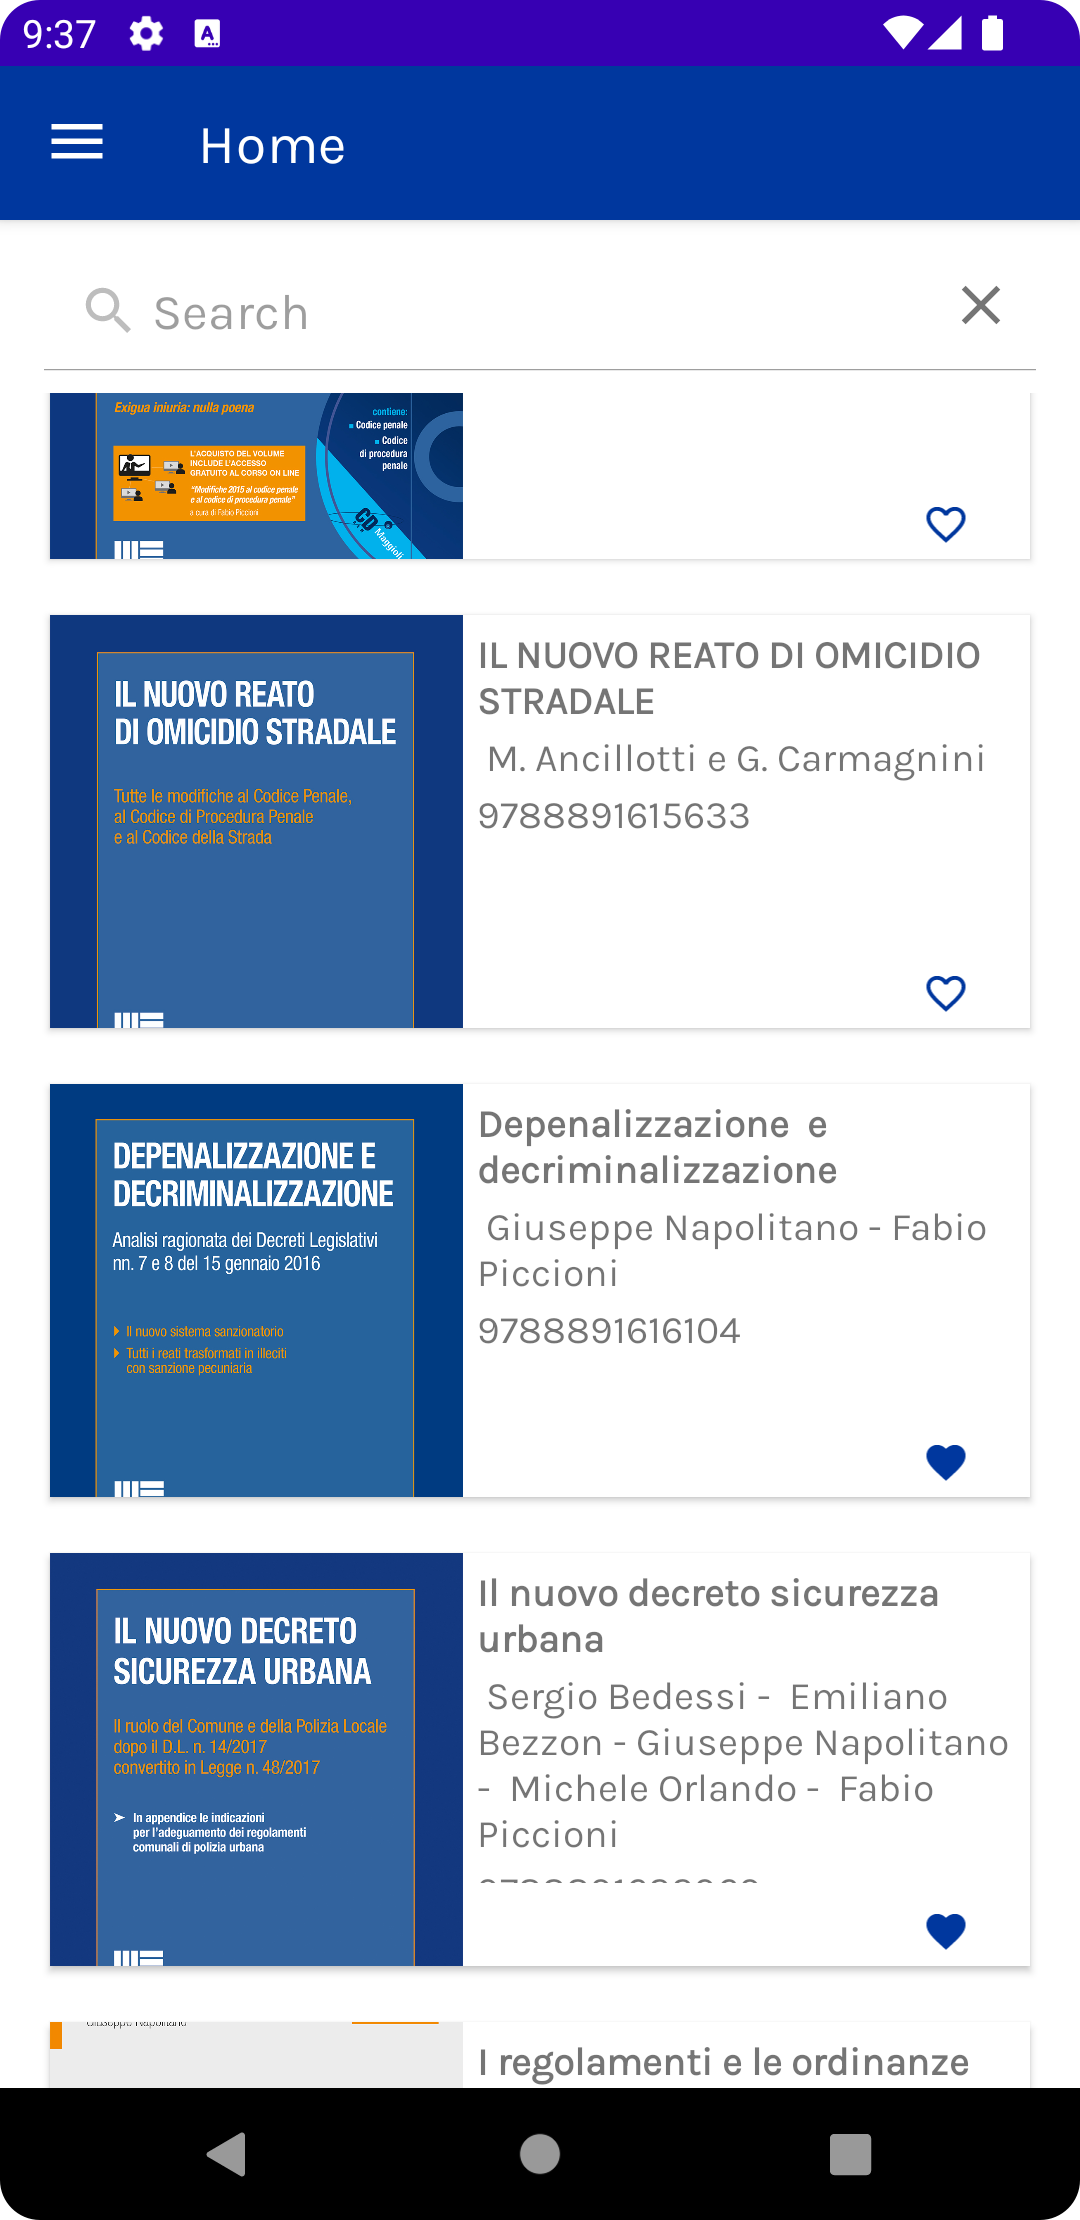
\includegraphics[width=0.21\textwidth]{img/home.png}
                \caption{Schermata home principale per la visualizzazione e la ricerca dei documenti digitali Maggioli}
                \label{home}
            \end{figure}
            
            \begin{figure}[H]
                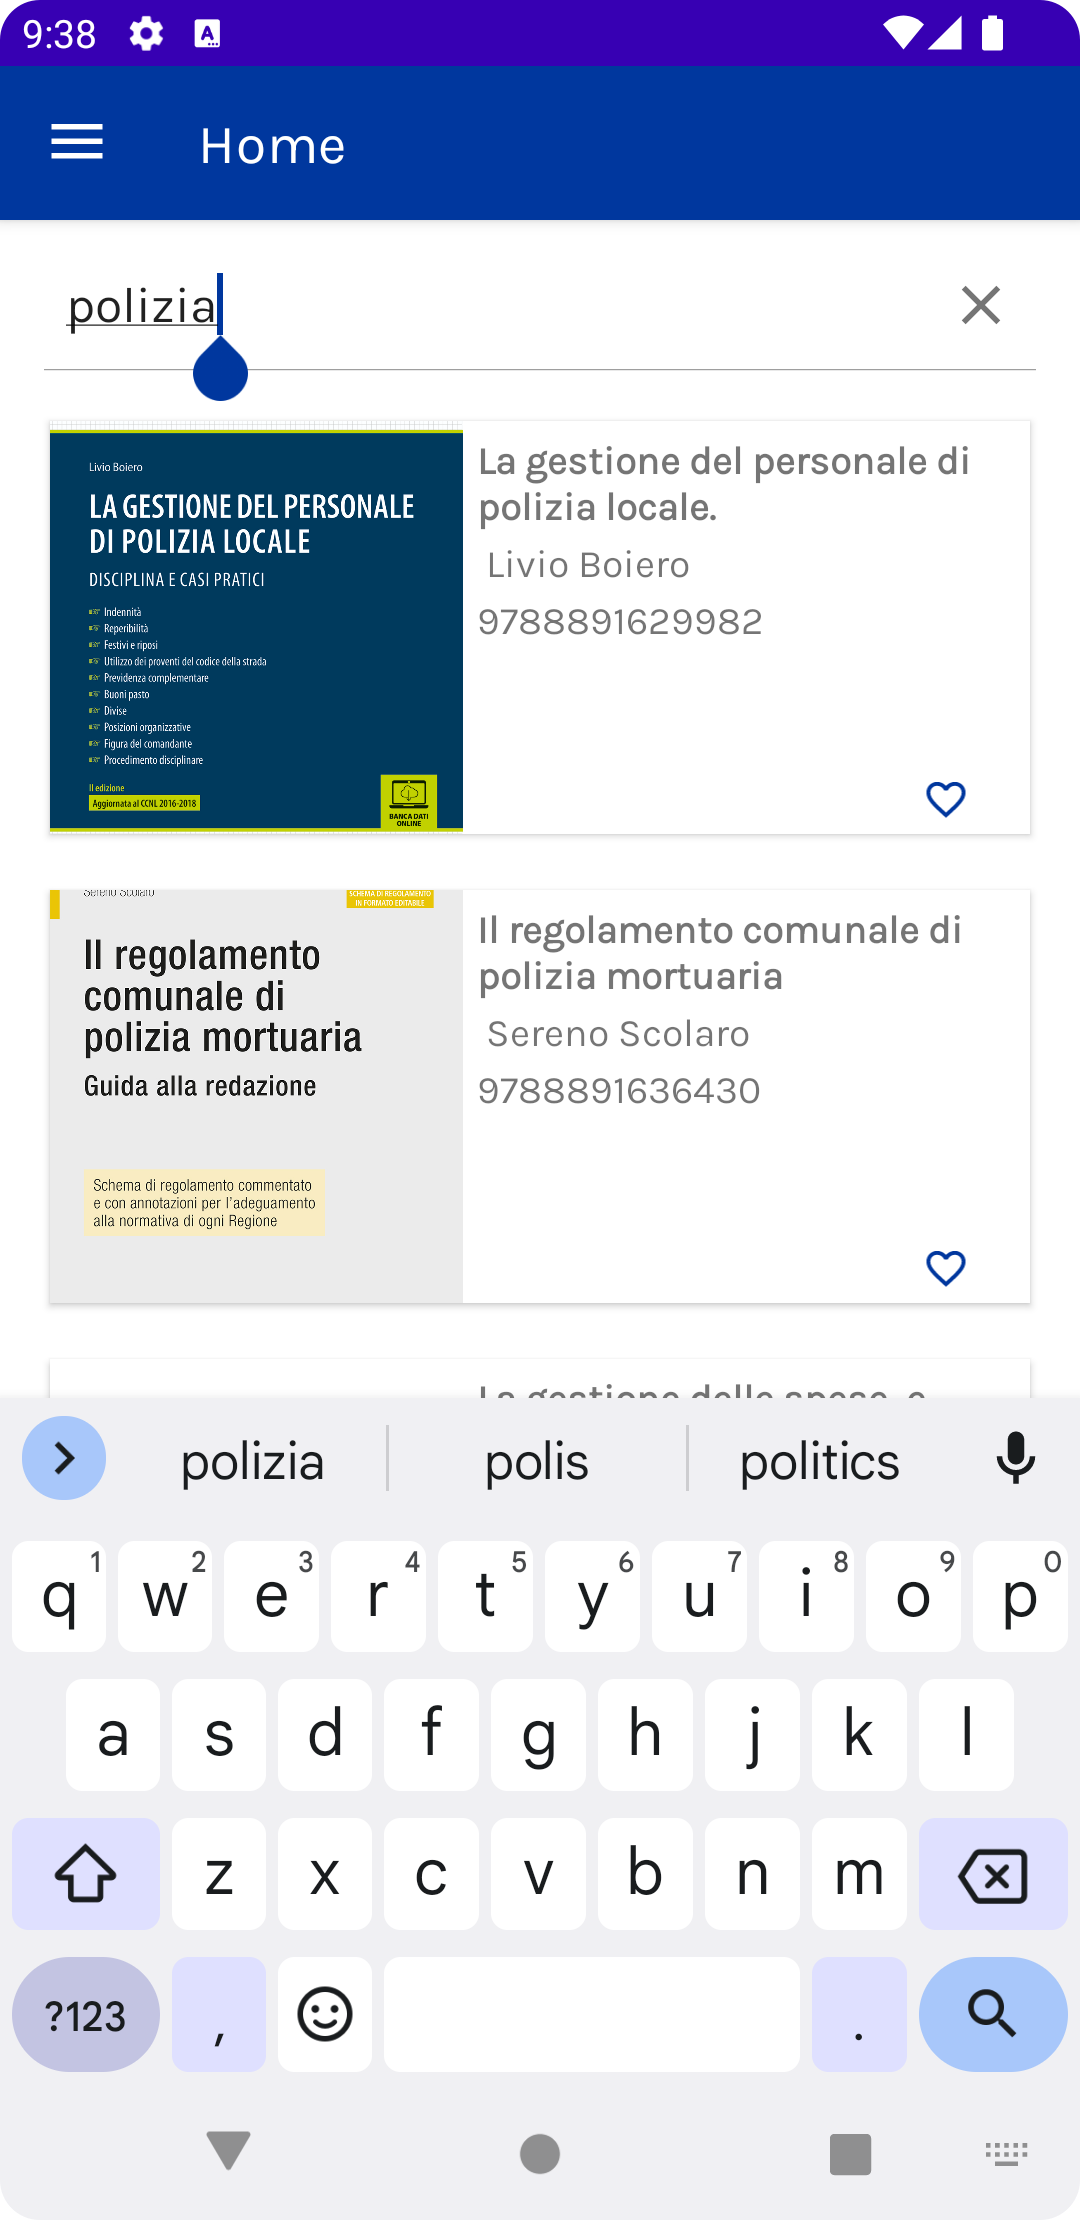
\includegraphics[width=0.21\textwidth]{img/ricerca.png}
                \caption{Esempio di ricerca per parola chiave nella schermata principale}
                \label{ricerca}
            \end{figure}

            \begin{figure}[H]
                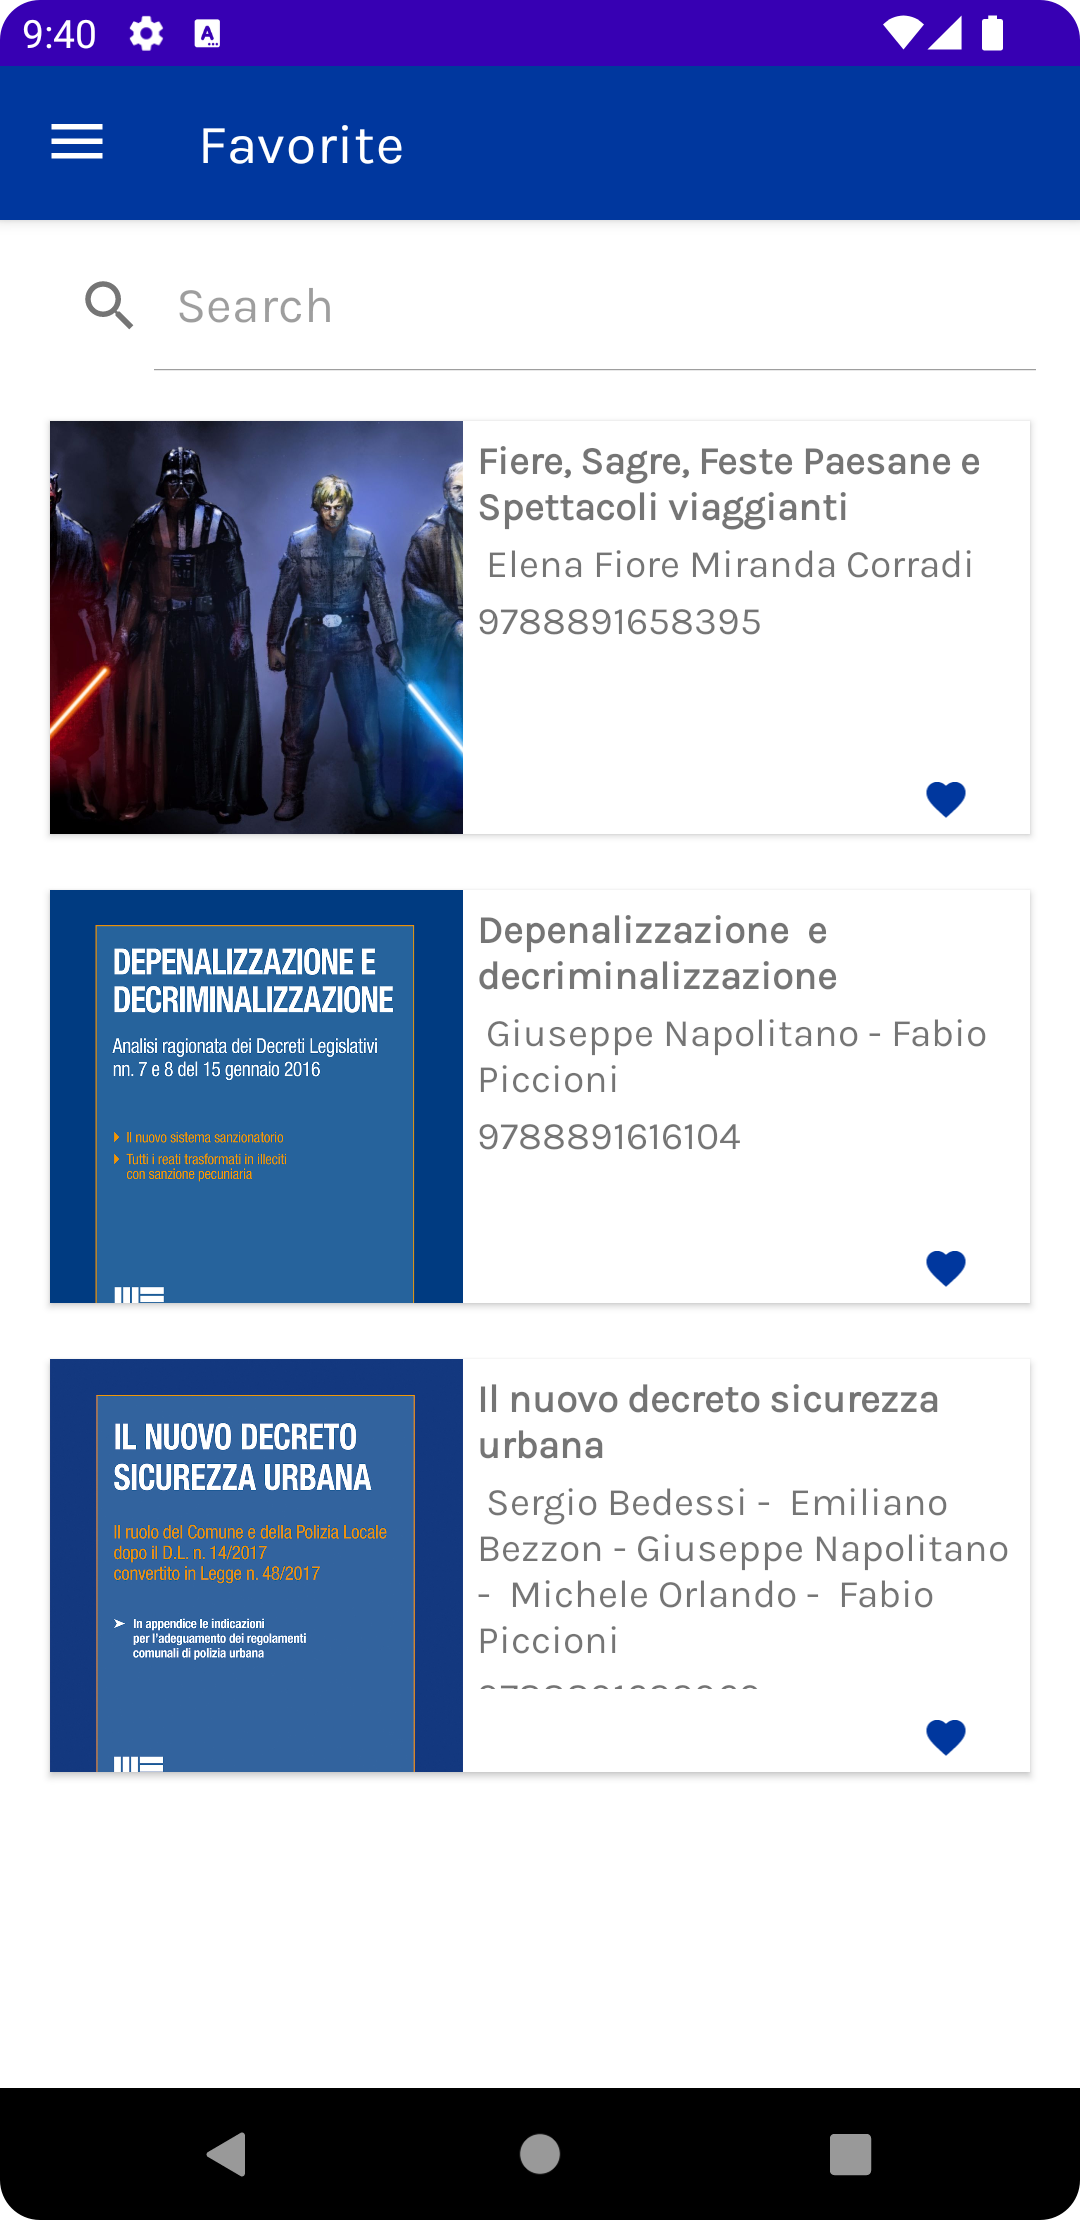
\includegraphics[width=0.21\textwidth]{img/preferiti.png}
                \caption{Schermata per la visualizzazione e la ricerca dei documenti preferiti dall'utente}
                \label{preferiti}
            \end{figure}

            \begin{figure}[H]
                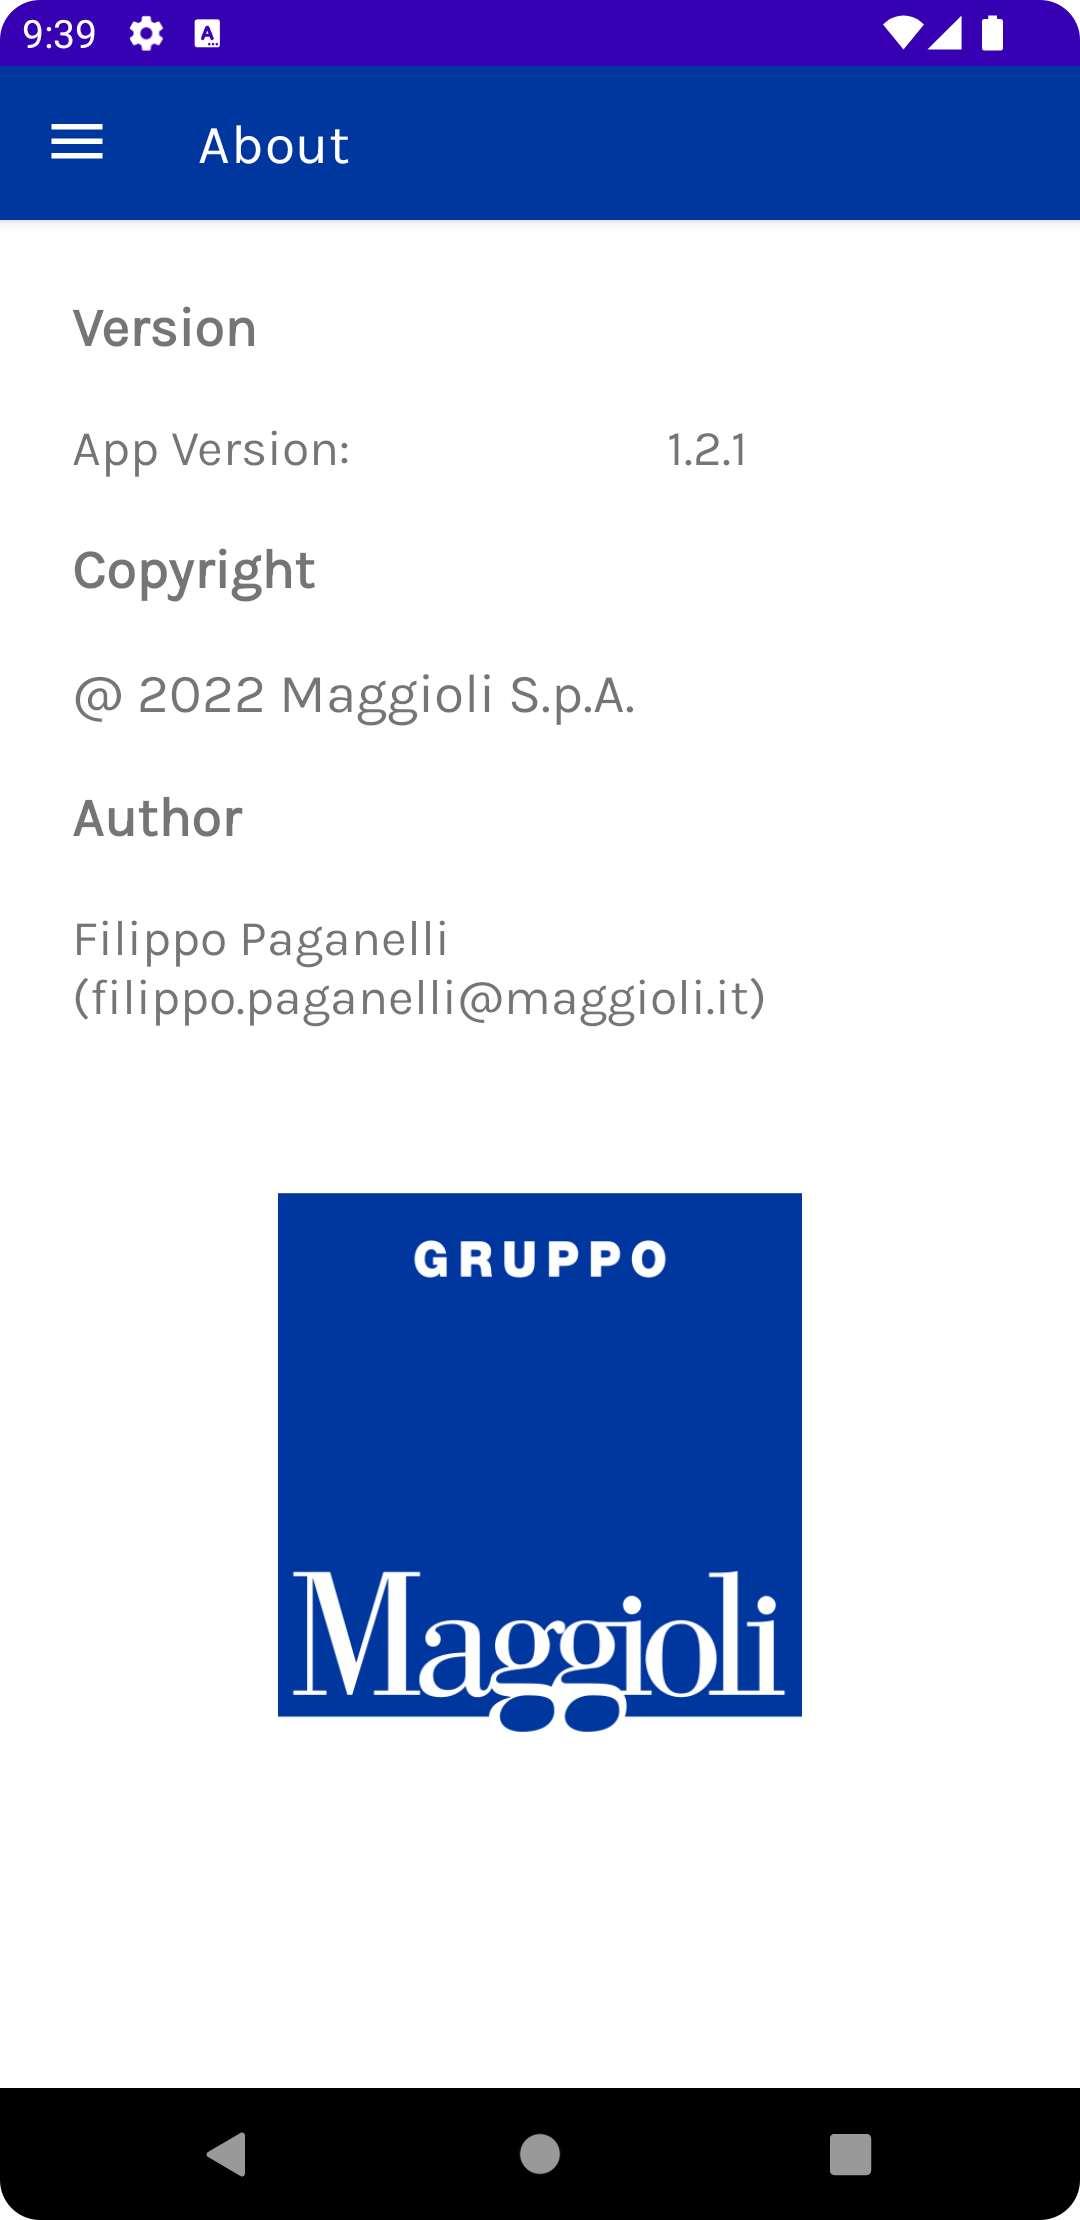
\includegraphics[width=0.21\textwidth]{img/about.png}
                \caption{Schermata per la visualizzazione delle informazioni generali relative alla applicazione}
                \label{about}
            \end{figure}

            \begin{figure}[H]
                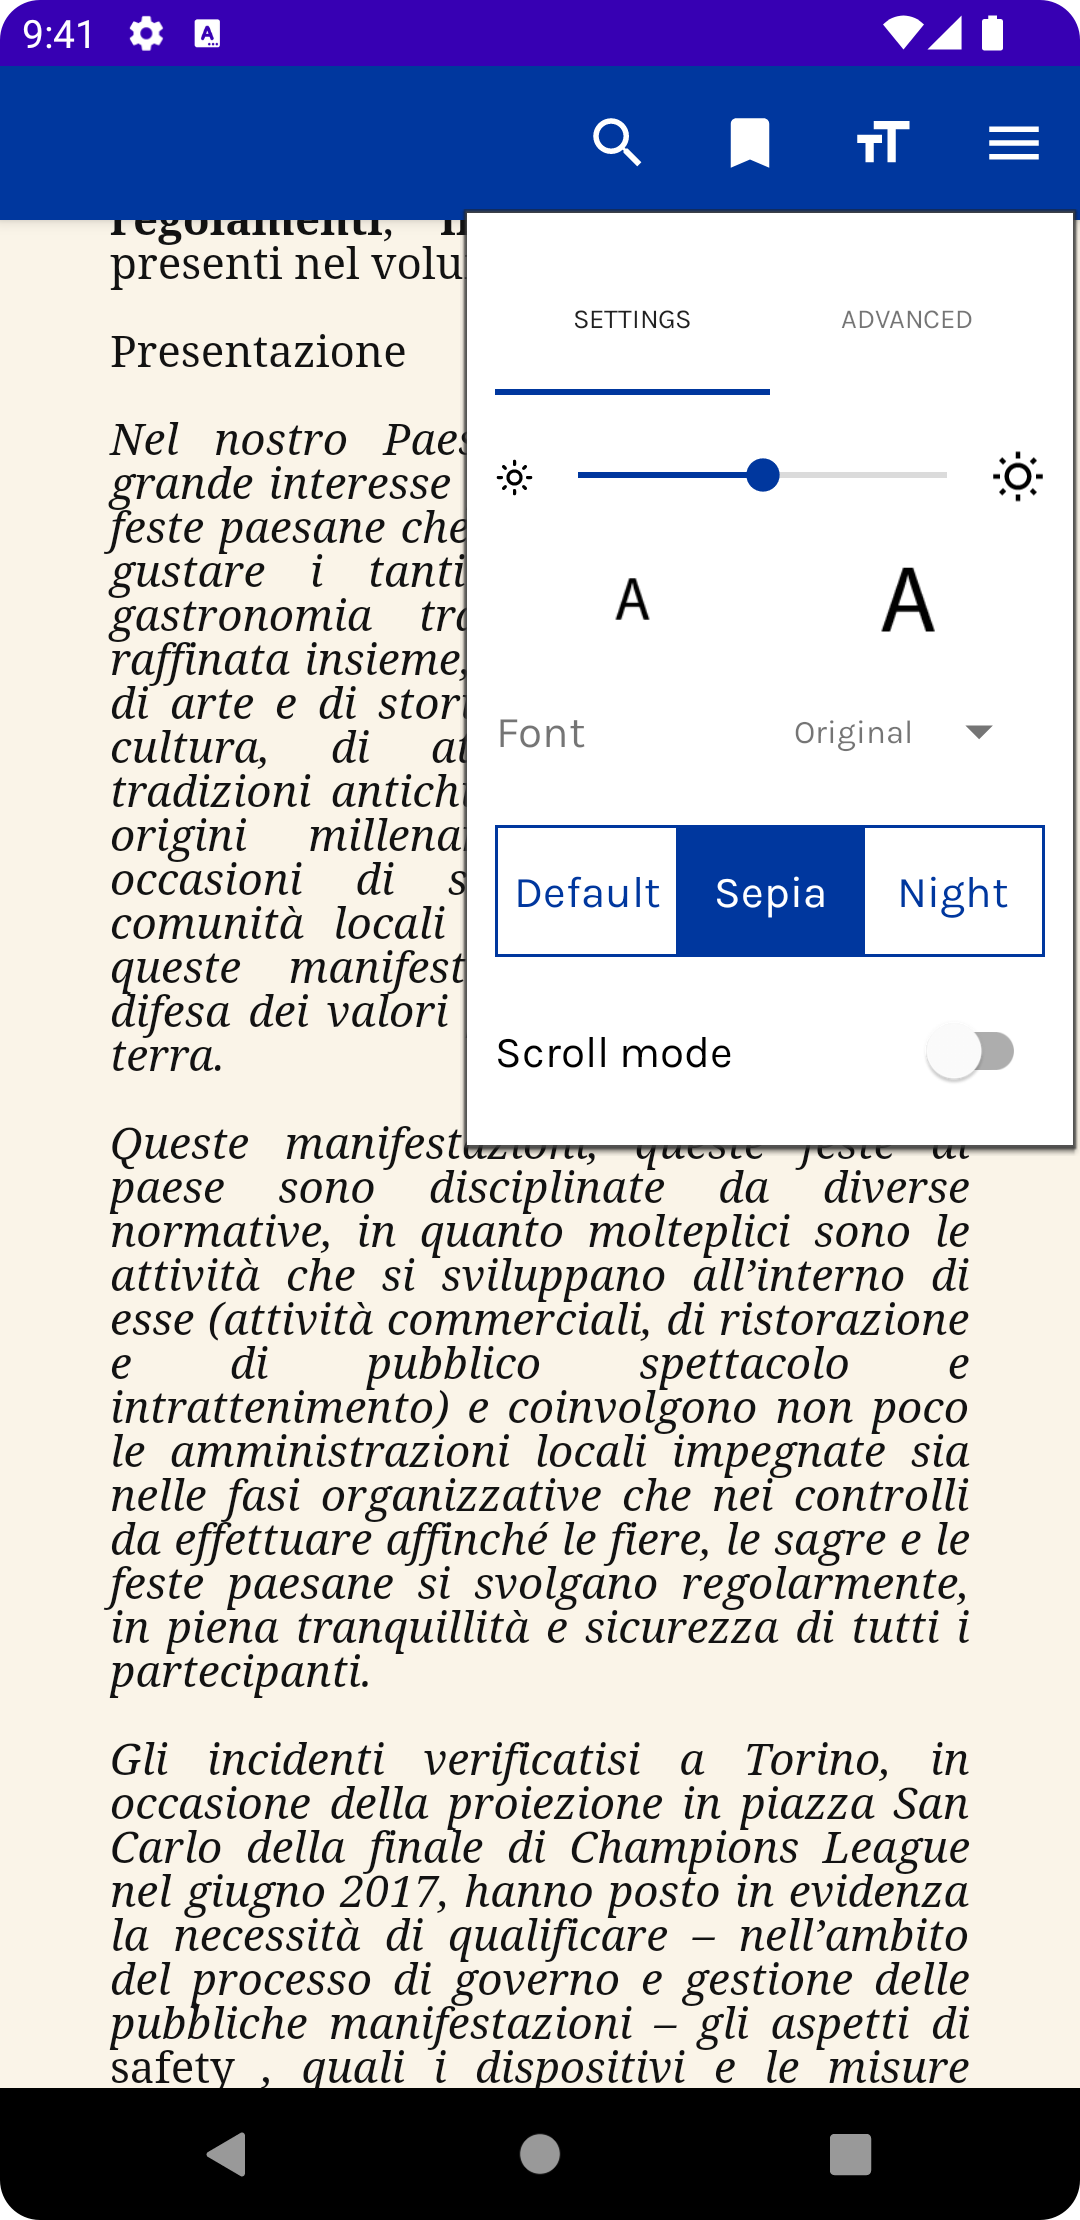
\includegraphics[width=0.21\textwidth]{img/reader_settings.png}
                \caption{Lettura documento digitale d'esempio e impostazioni del lettore}
                \label{readersettings}
            \end{figure}
            
            \begin{figure}[H]
                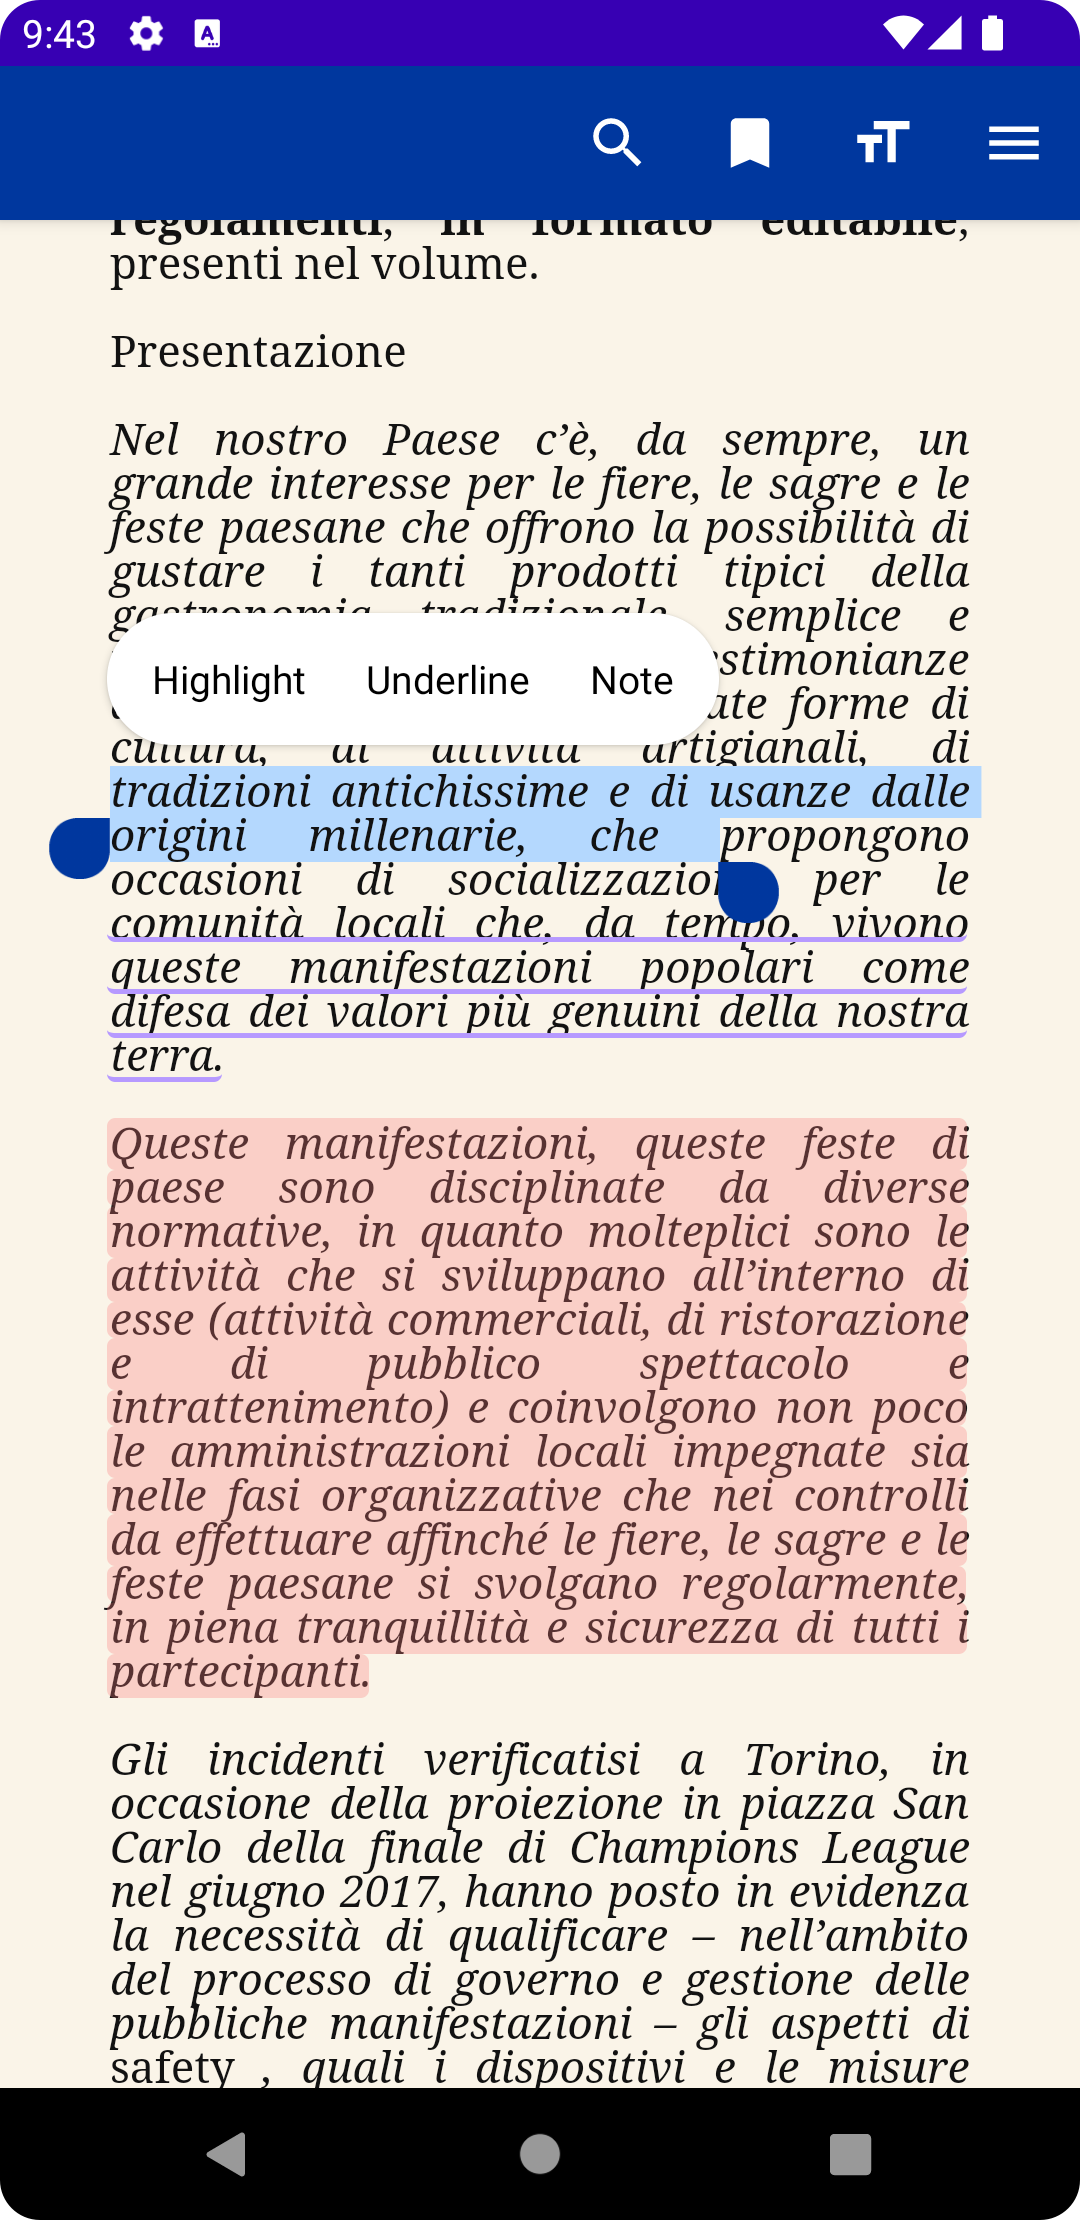
\includegraphics[width=0.21\textwidth]{img/annotations.png}
                \caption{Esempio di inserimento di annotazioni come evidenziazioni e sottolineature}
                \label{annotations}
            \end{figure}
            
            \begin{figure}[H]
                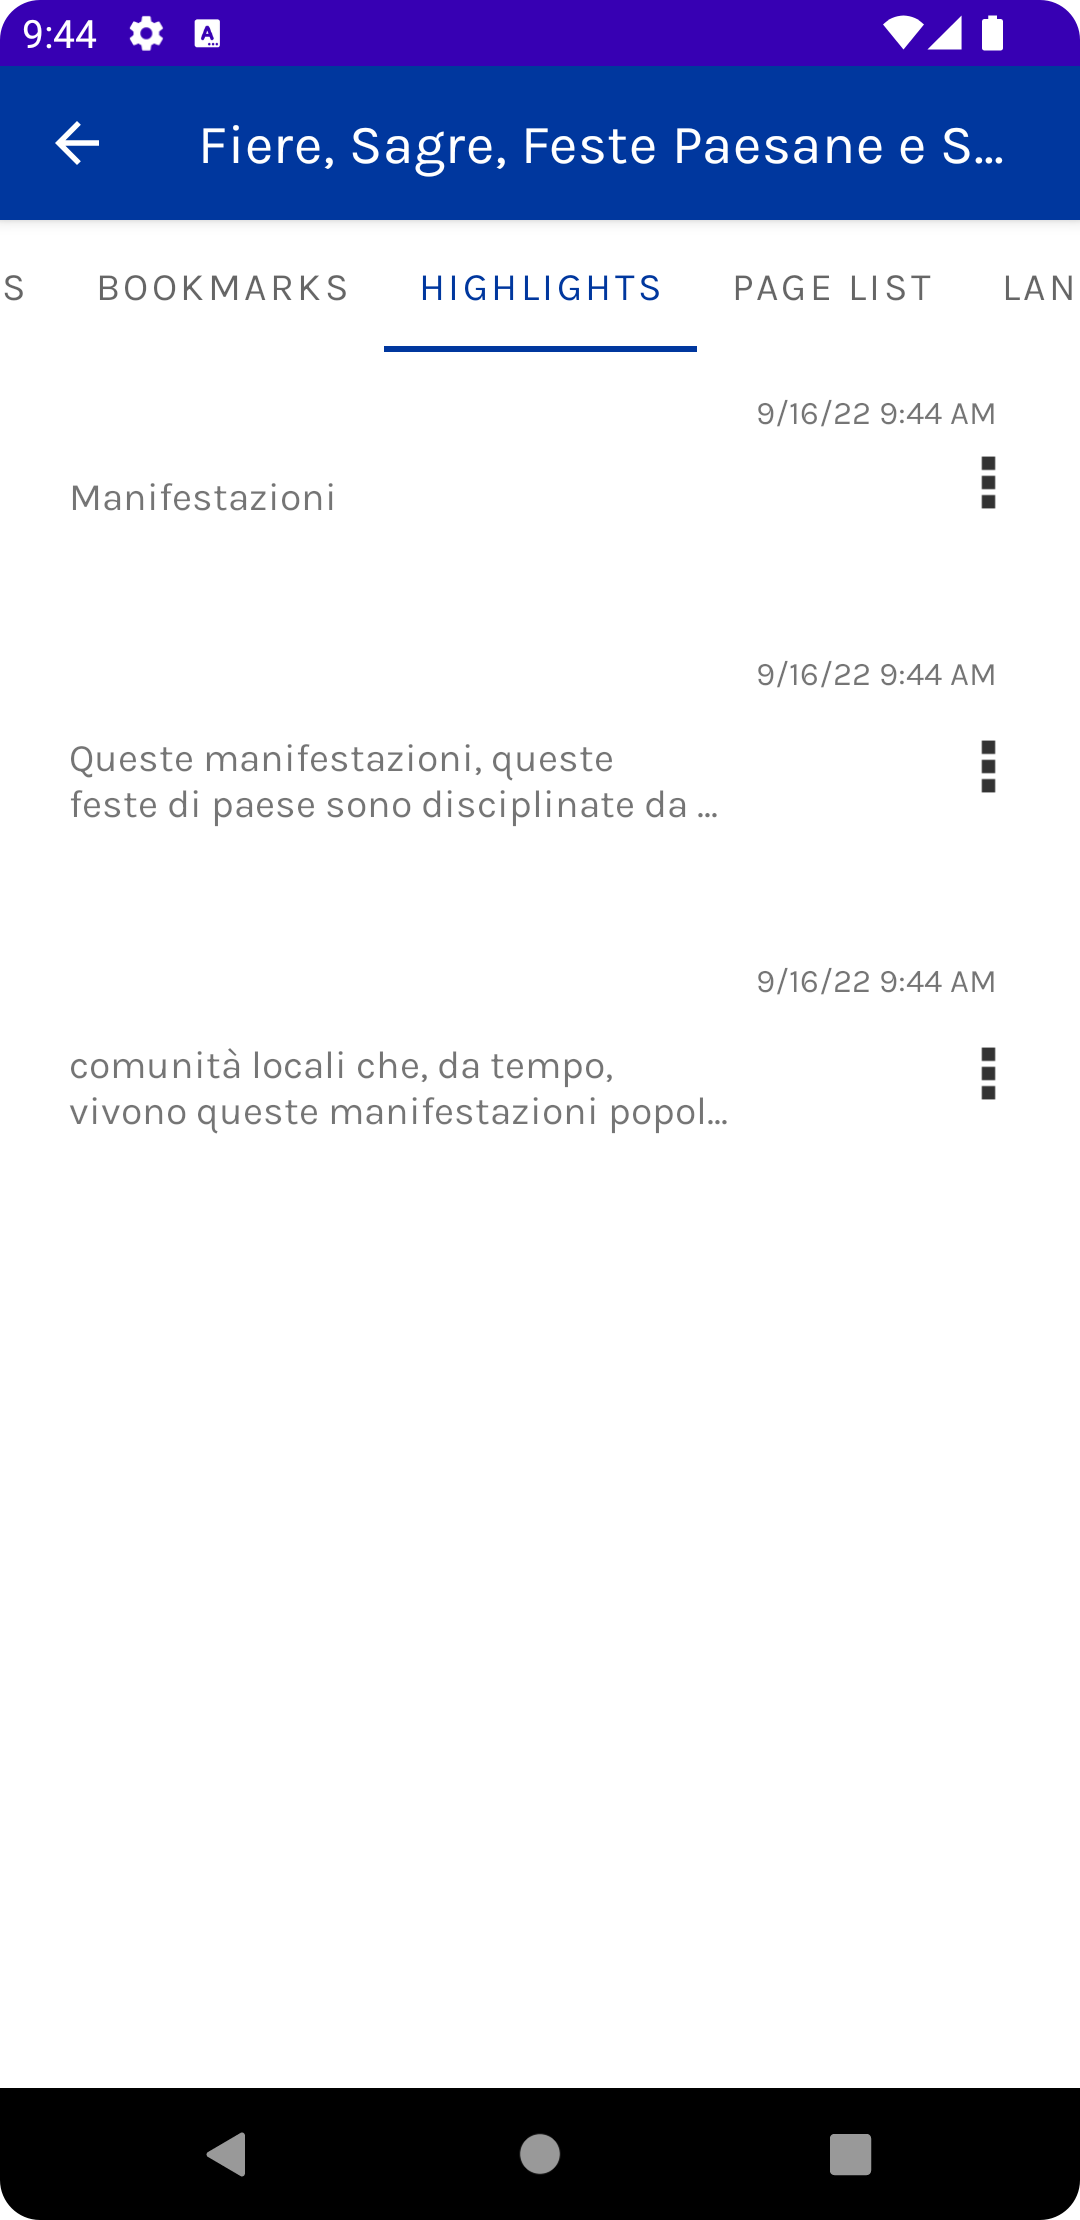
\includegraphics[width=0.21\textwidth]{img/annotation2.png}
                \caption{Annotazioni memorizzate sul dispositivo e consultabili dal menu del lettore}
                \label{annotation2}
            \end{figure}

            \begin{figure}[H]
                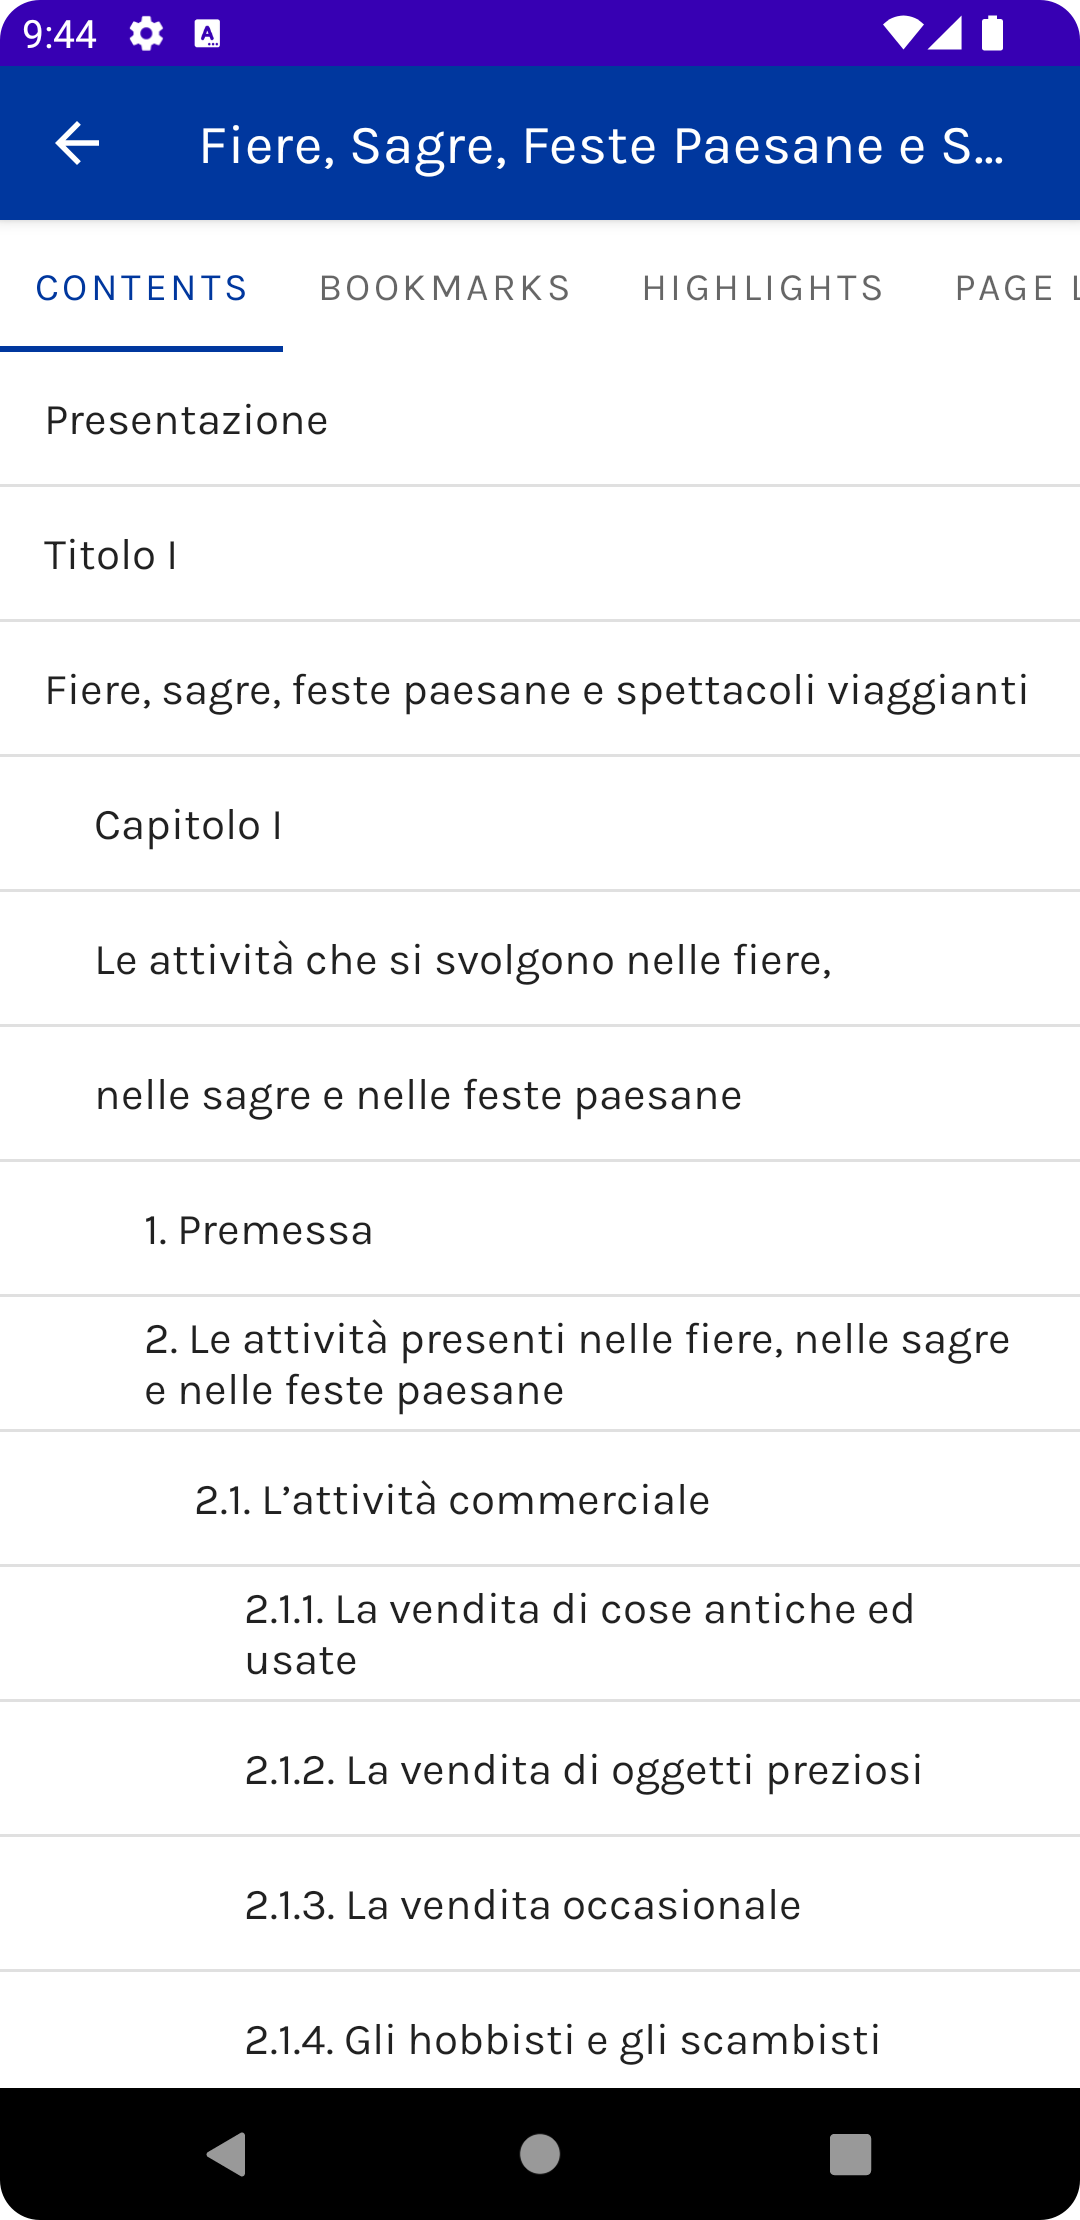
\includegraphics[width=0.21\textwidth]{img/toc.png}
                \caption{Elenco dei contenuti (TOC) del documento aperto e consultabile dal menu del lettore}
                \label{toc}
            \end{figure}
            
            \begin{figure}[H]
                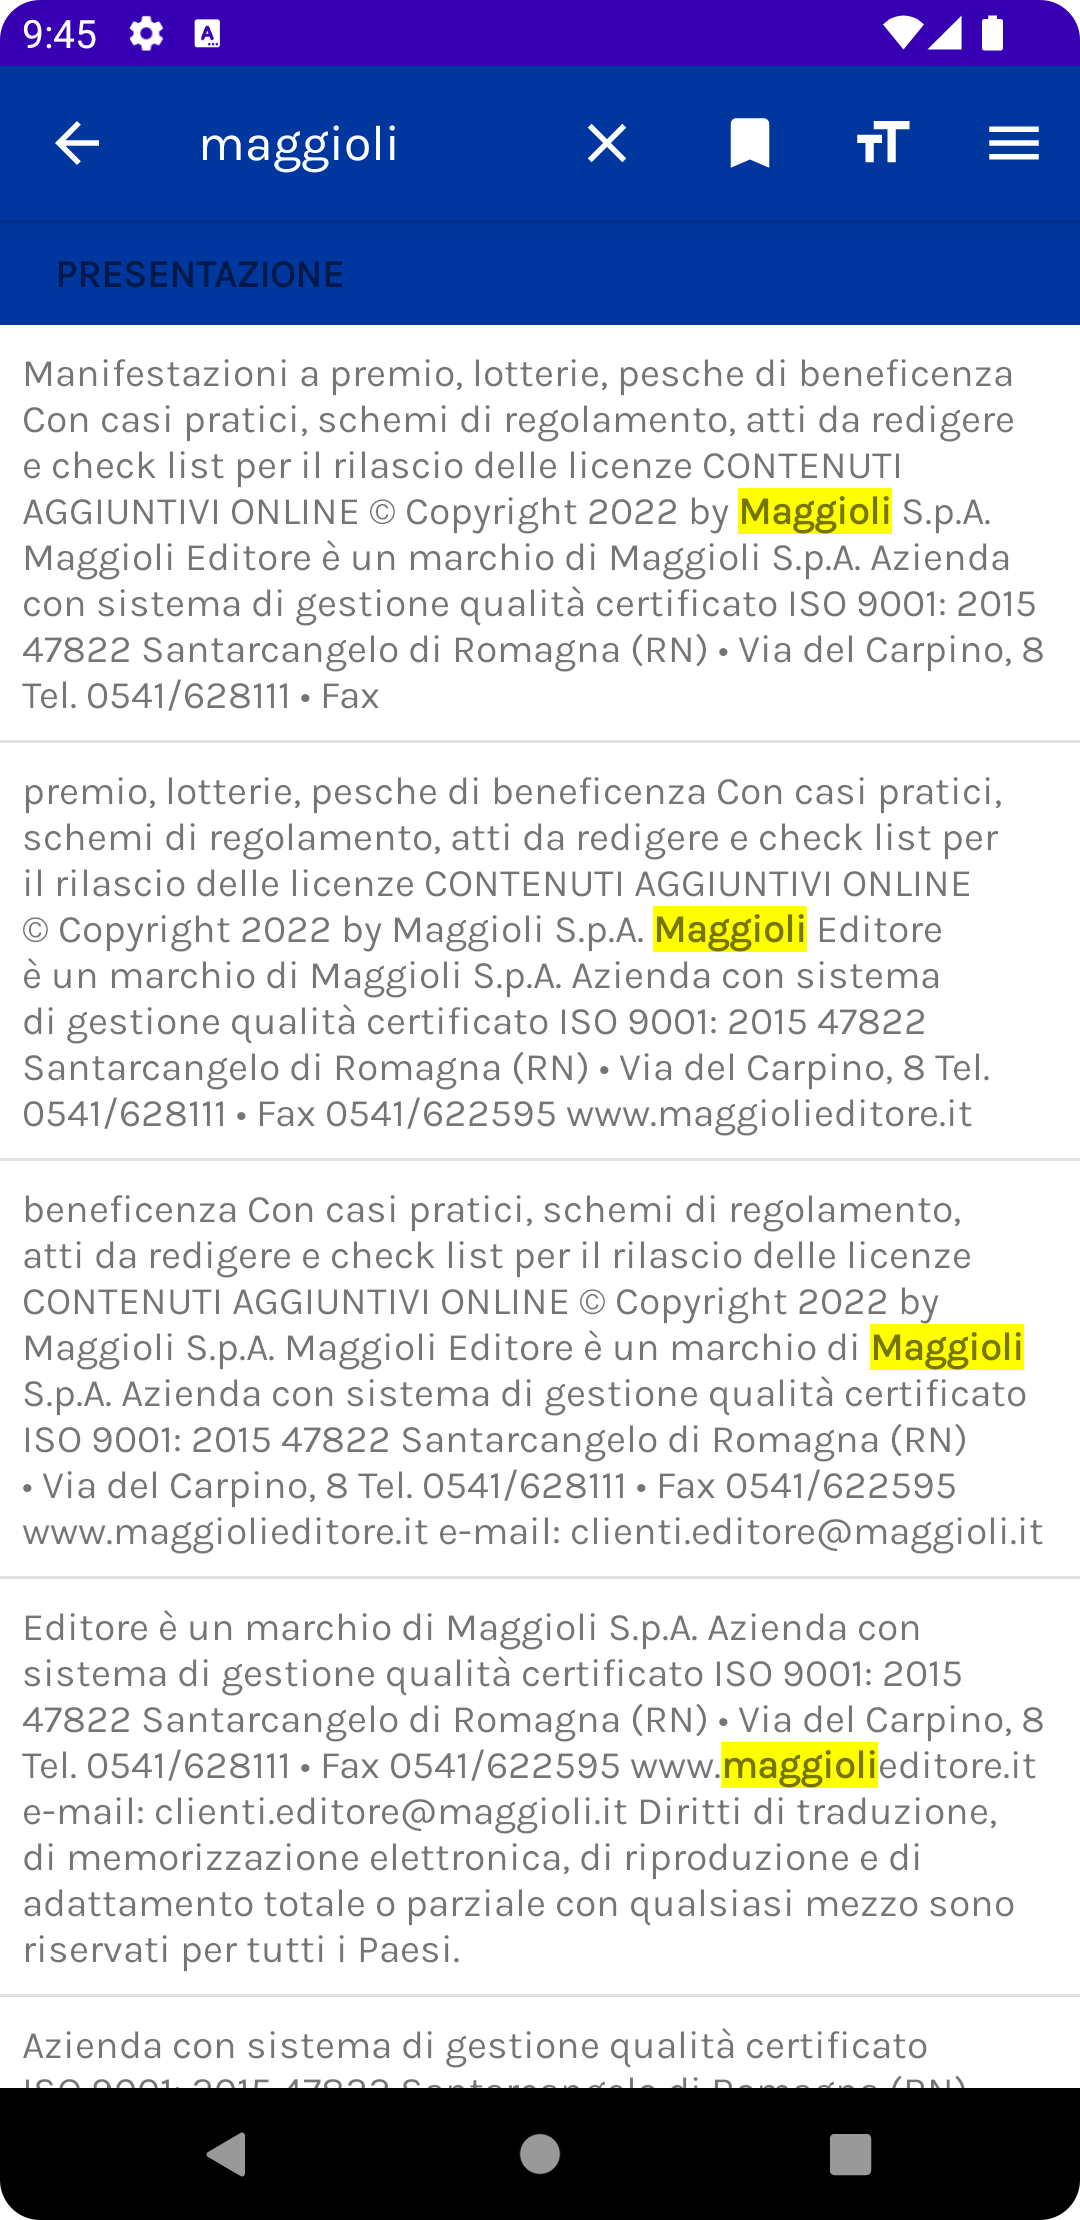
\includegraphics[width=0.21\textwidth]{img/ricerca_testo.png}
                \caption{Ricerca testuale nel contenuto del documento aperto con relativo risultato}
                \label{ricerca_testo}
            \end{figure}
            
            \begin{figure}[H]
                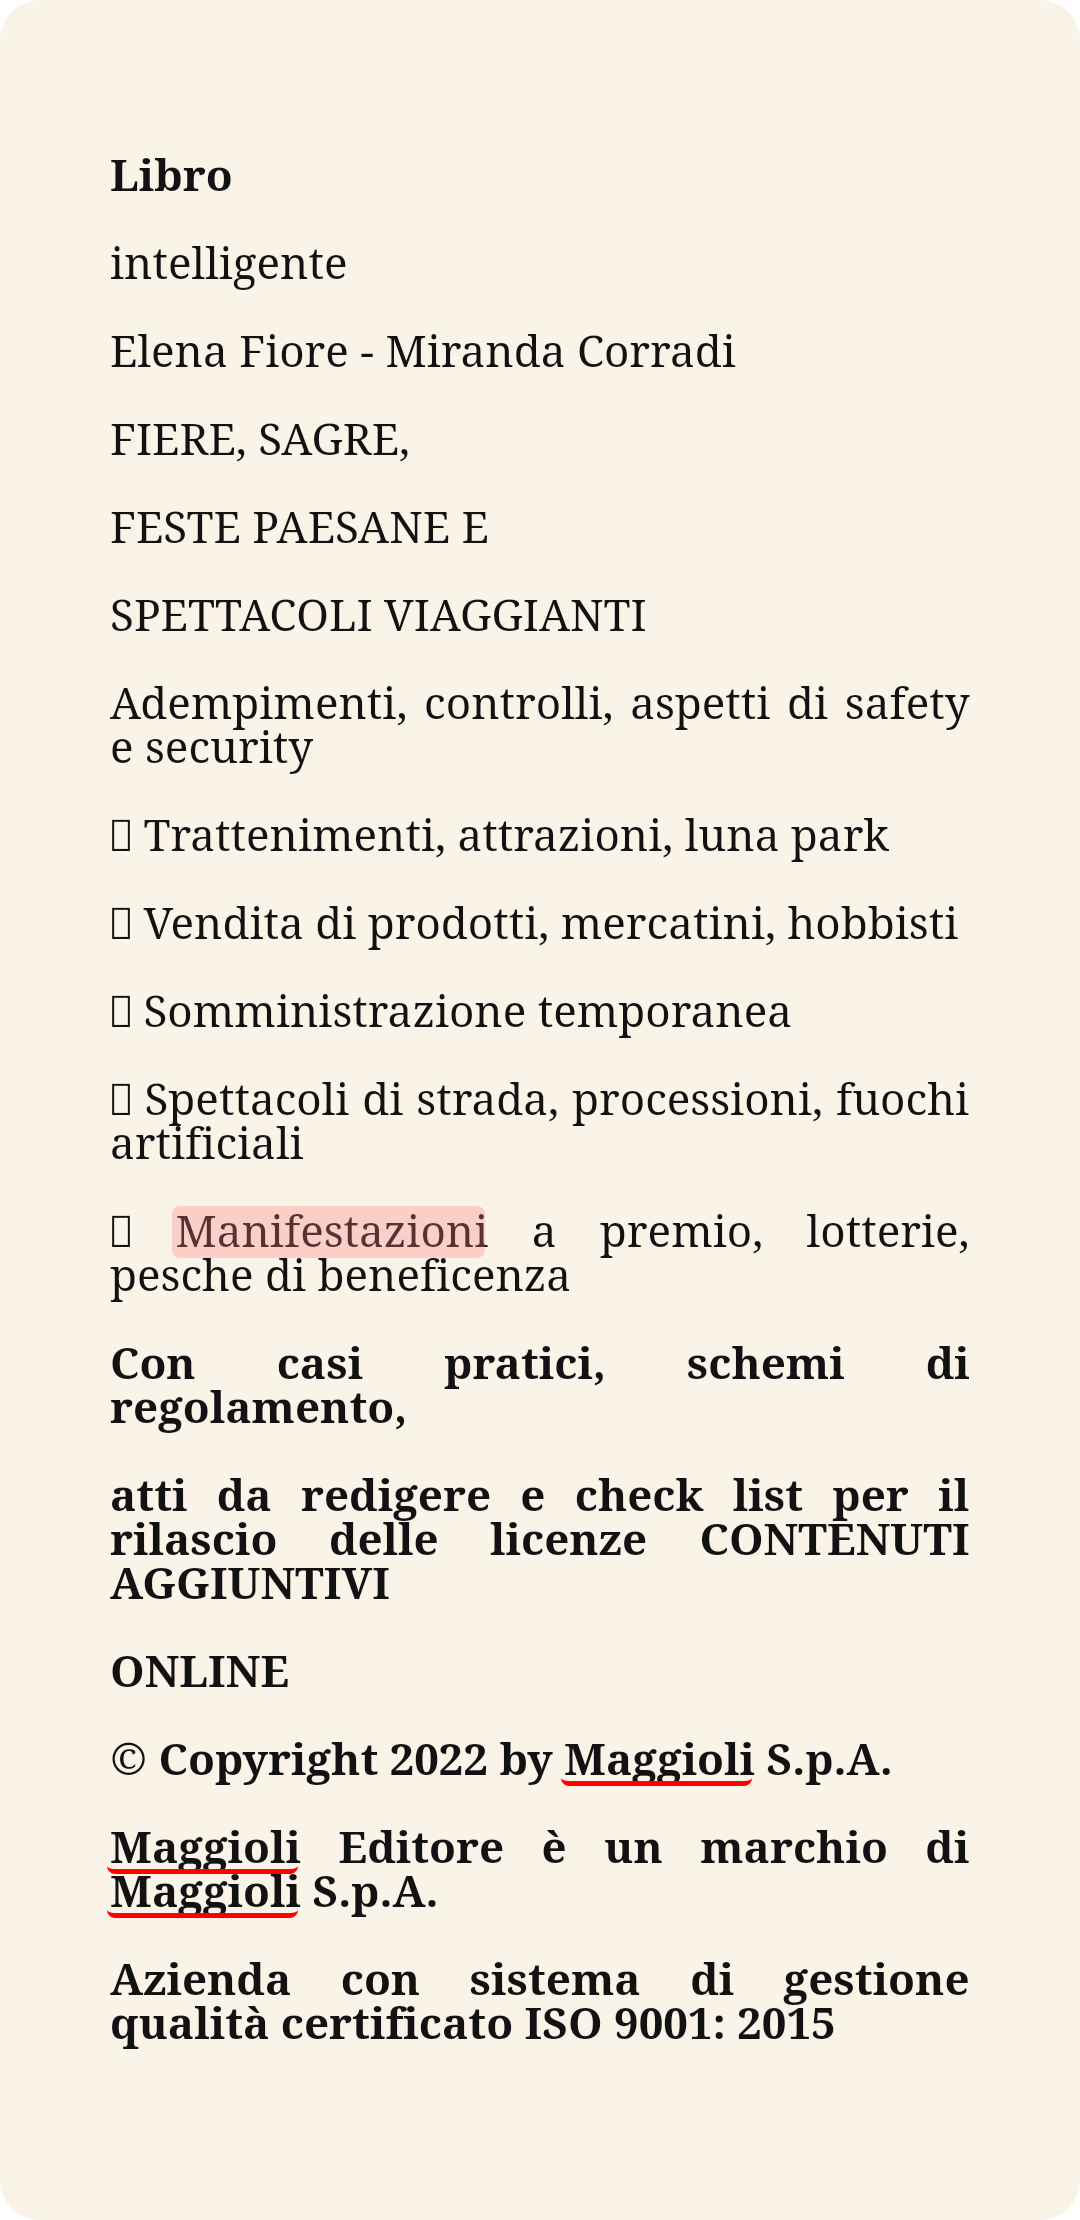
\includegraphics[width=0.21\textwidth]{img/ricerca_testo2.png}
                \caption{Evidenziazioni automatiche delle occorrenze del testo cercato}
                \label{ricerca_testo2}
            \end{figure}
\end{multicols}

\subsection{iosMaggioliEbookApp}

Per poter sviluppare l'interfaccia grafica della applicazione per la versione iOS è possibile aprire il progetto \textit{iosMaggioliEbookApp} con Xcode. Il contenuto di questa cartella è stato generato in modo automatico durante l'inizializzazione dell'intero progetto con il plugin gradle KMM (come descritto nel capitolo \ref{ch:ch3}).\\
L'IDE Xcode deve essere configurato per poter utilizzare il codice condiviso sviluppato nel modulo shared: a tale scopo il plugin gradle KMM fornisce un apposito task che deve essere utilizzato in fase di compilazione. Il task \textit{embedAndSignPodAppleFrameworkForXcode} è visibile solo a Xcode e permette di esporre il framework al progetto Xcode per il quale è stata creata l'applicazione iOS. Utilizzando la configurazione del progetto iOS questo task definisce la modalità di compilazione (debug o release) e fornisce la versione del framework appropriata nella posizione specificata.\\
Tale posizione (\textit{\$(SRCROOT)/../shared/build/cocoapods/framework}) deve poi essere configurata nella sezione "\textit{Build Settings|Framework Search Paths}" in modo da indicare a XCode il percorso corretto per la ricerca del framework compilato a partire dal modulo condiviso.

\begin{listing}[H]
\inputminted{bash}{code/5-xcodeconfigkmm}
\caption{Configurazione build script custom in Xcode tramite l'apposito task del plugin Gradle KMM ("\textit{Build Phases|Run Script}").}
\end{listing}

\subsubsection{CocoaPods}
Dopo aver aggiornato lo script di configurazione è necessario installare il modulo shared, il quale è impacchettato come dipendenza\textit{CocoaPods}\footnote{\url{https://cocoapods.org/}}. CocoaPods è un dependency manager per progetti Swift e Objective-C scritto in Ruby. Le dipendenze, chiamate \textit{Pods}, sono definite nel file \textit{Podfile} nella root di progetto. Il pod shared viene generato durante la fase di impacchettamento del modulo shared tramite l'esecuzione del task \textit{gradle assemble} per il quale sono definiti appositi sottotask per svolgere questo compito. I task forniti dal plugin Gradle KMM per la gestione delle dipendenze CocoaPods sono:
\begin{itemize}
    \item \textit{podDownload} - Scarica le dipendenze CocoaPods senza effettuarne l'installazione.
    \item \textit{podImport} - Task di utility utilizzato dal altri task per l'import delle dipendenze.
    \item \textit{podInstall} - Esegue l'installazione dei pod (equivalente all'esecuzione del comando \textit{pod install}
    \item \textit{podPublishDebugXCFramework} - Crea il framework XCFramework in modalità debug (chiamato dal task \textit{embedAndSignPodAppleFrameworkForXcode}).
    \item \textit{podPublishReleaseXCFramework} - Crea il framework XCFramework in modalità release (chiamato dal task \textit{embedAndSignPodAppleFrameworkForXcode}).
    \item \textit{podPublishXCFramework} - Crea i framework XCFrameworc in entrambe le modalità.
    \item \textit{podspec} - Genera il file \textit{podspec}\footnote{\url{https://guides.cocoapods.org/syntax/podspec.html}}, utile all'importazione del pod nella applicazione iOS.
\end{itemize}

Il seguente file definisce i pods della applicazione iOS, compreso il modulo shared, il quale deve essere incluso localmente:

% aggiornare listings con podfile finale
\begin{listing}[H]
\inputminted{bash}{code/5-podfile}
\caption{Dipendenze CocoaPods della applicazione iOS.}
\end{listing}
A questo punto è possibile importare i moduli nel codice Swift e sviluppare l'applicazione utilizzando le funzionalità fornite dall'IDE a supporto dello sviluppo come per una qualsiasi libreria Swift importata.

\subsubsection{Architettura iOS}
% descrivere architettura app ios MVVM con navigation (identica a android)
view + viewmodel e navigazione con navigationview + navigationlink (deprecato in favore di navigationstack e navigationsplitview

ZStack per navcontroller e sidebar in modo da far vedere la sidebar in overlay rispetto alle views. navcontroller è navigationview e sostituisco le views tramite i navigation link che si trovano nella sidebar

mi sono implementato da solo il paging per lo scroll infinito

\subsubsection{Integrazione iOS-Shared}
% descrivere gestione coroutine kotlin in runtime ios
ho dovuto fare oggetto per convertire bytearray in data (per mostrare le cover) + oggetto per caricarle in modo async una volta scaricata (simile a funzionamento della nuova api AsyncImage fornita da Swiftui nuovo)

Ho dovuto impostare \textit{kotlin.native.binary.memoryModel=experimental} nel file \textit{gradle.properties} per il modulo condiviso. Senza questa configurazione ottenevo l'errore "\textit{Uncaught Kotlin exception: kotlin.IllegalStateException: There is no event loop. Use runBlocking \{ ... \} to start one.}"\footnote{\url{https://github.com/JetBrains/kotlin/blob/master/kotlin-native/NEW_MM.md\#enable-the-new-mm}}.

ho dovuto fare una extensions al libro per dire quale è l'id usato da identifiable in modo da poter ciclare su liste di libri

\begin{listing}[H]
\inputminted{swift}{code/5-swift-shared}
\caption{Esempio di utilizzo dei casi d'uso del modulo condiviso (\textit{LoginViewModel.swift}).}
\end{listing}

\subsubsection{Screenshots}
\begin{multicols}{3}
            \begin{figure}[H]
                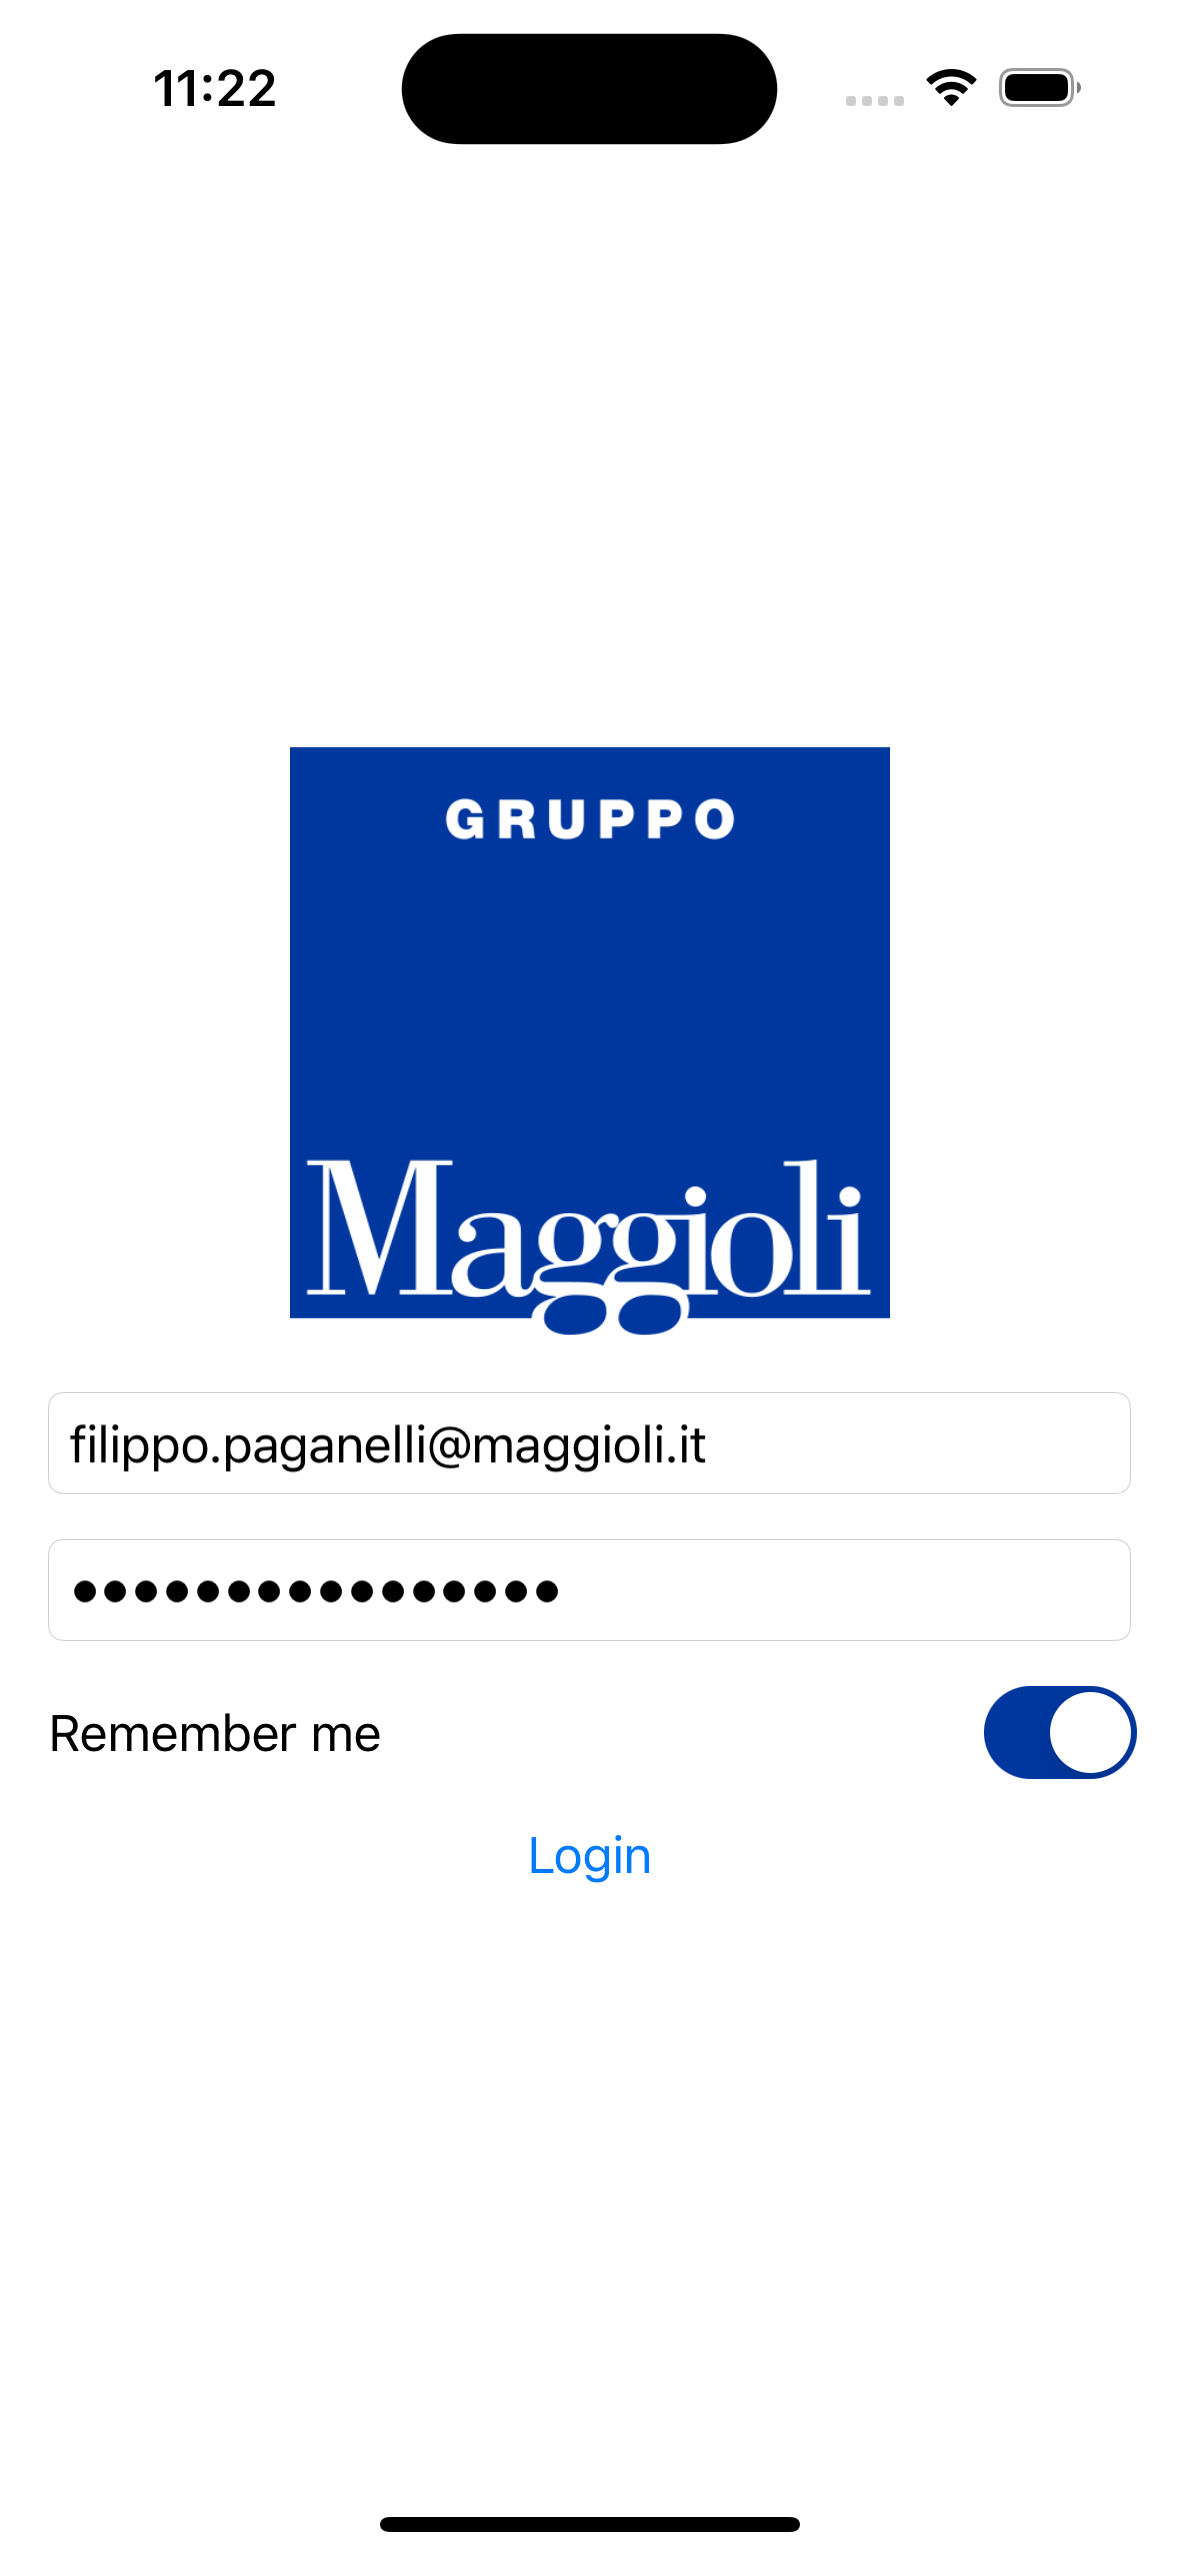
\includegraphics[width=0.21\textwidth]{img/Simulator Screen Shot - iPhone 14 Pro - 2022-10-05 at 11.22.08.png}
                \caption{Schermata di login degli utenti abbonati}
                \label{loginios}
            \end{figure}

            \begin{figure}[H]
                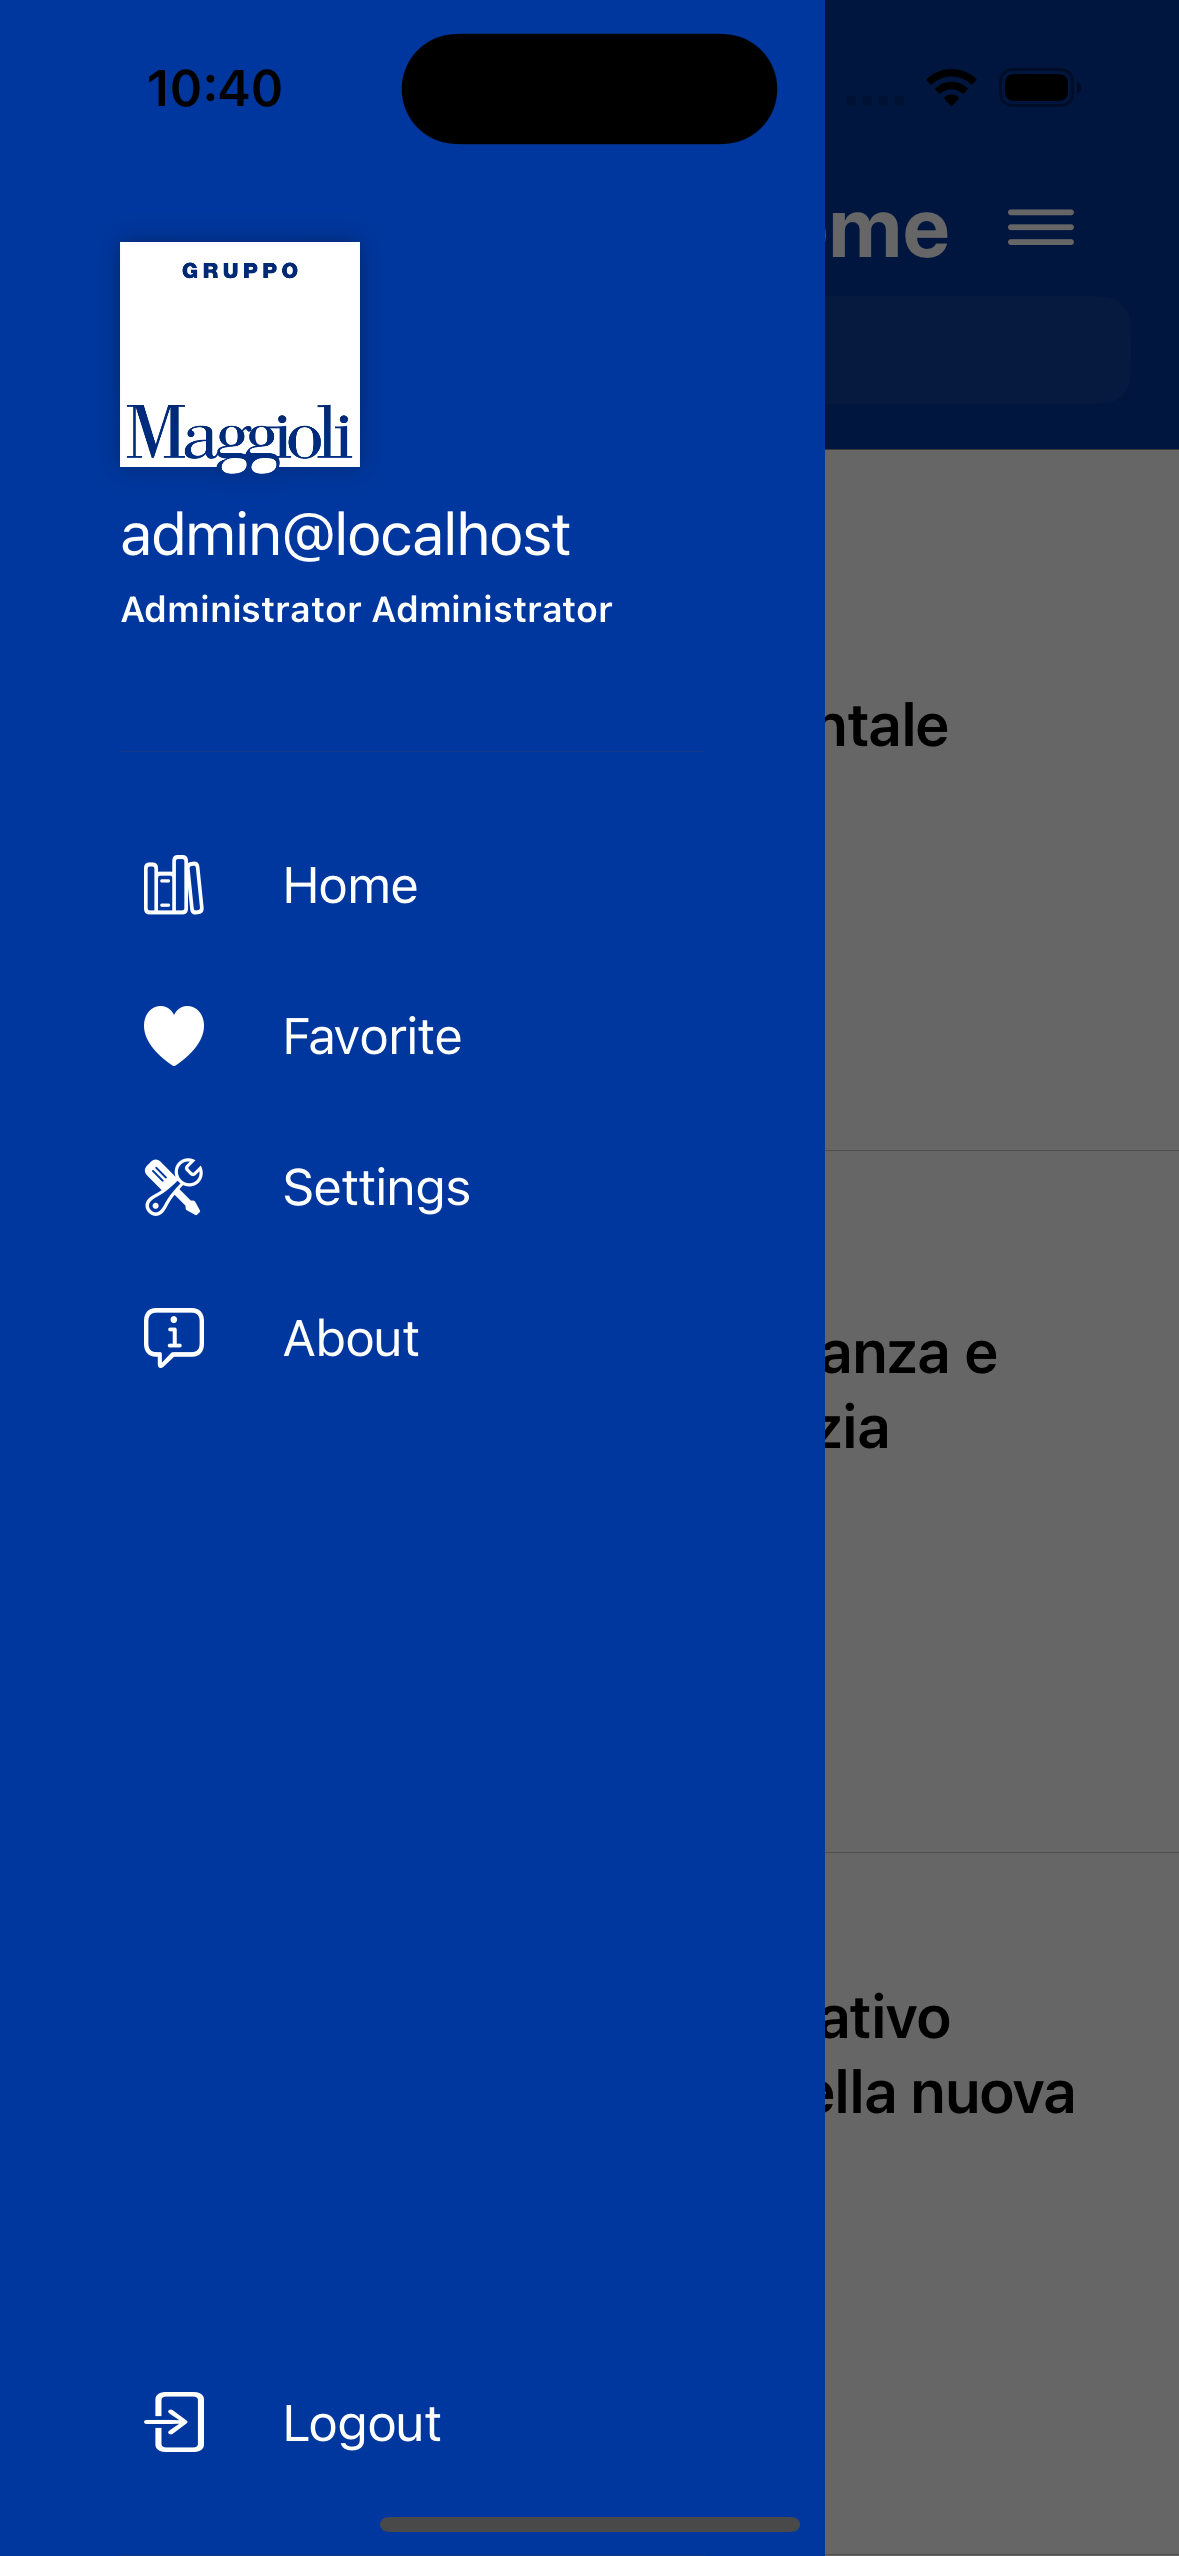
\includegraphics[width=0.21\textwidth]{img/Simulator Screen Shot - iPhone 14 Pro - 2022-10-05 at 10.40.04.png}
                \caption{Menu laterale per la navigazione all'interno della applicazione}
                \label{sidenavios}
            \end{figure}
            
            \begin{figure}[H]
                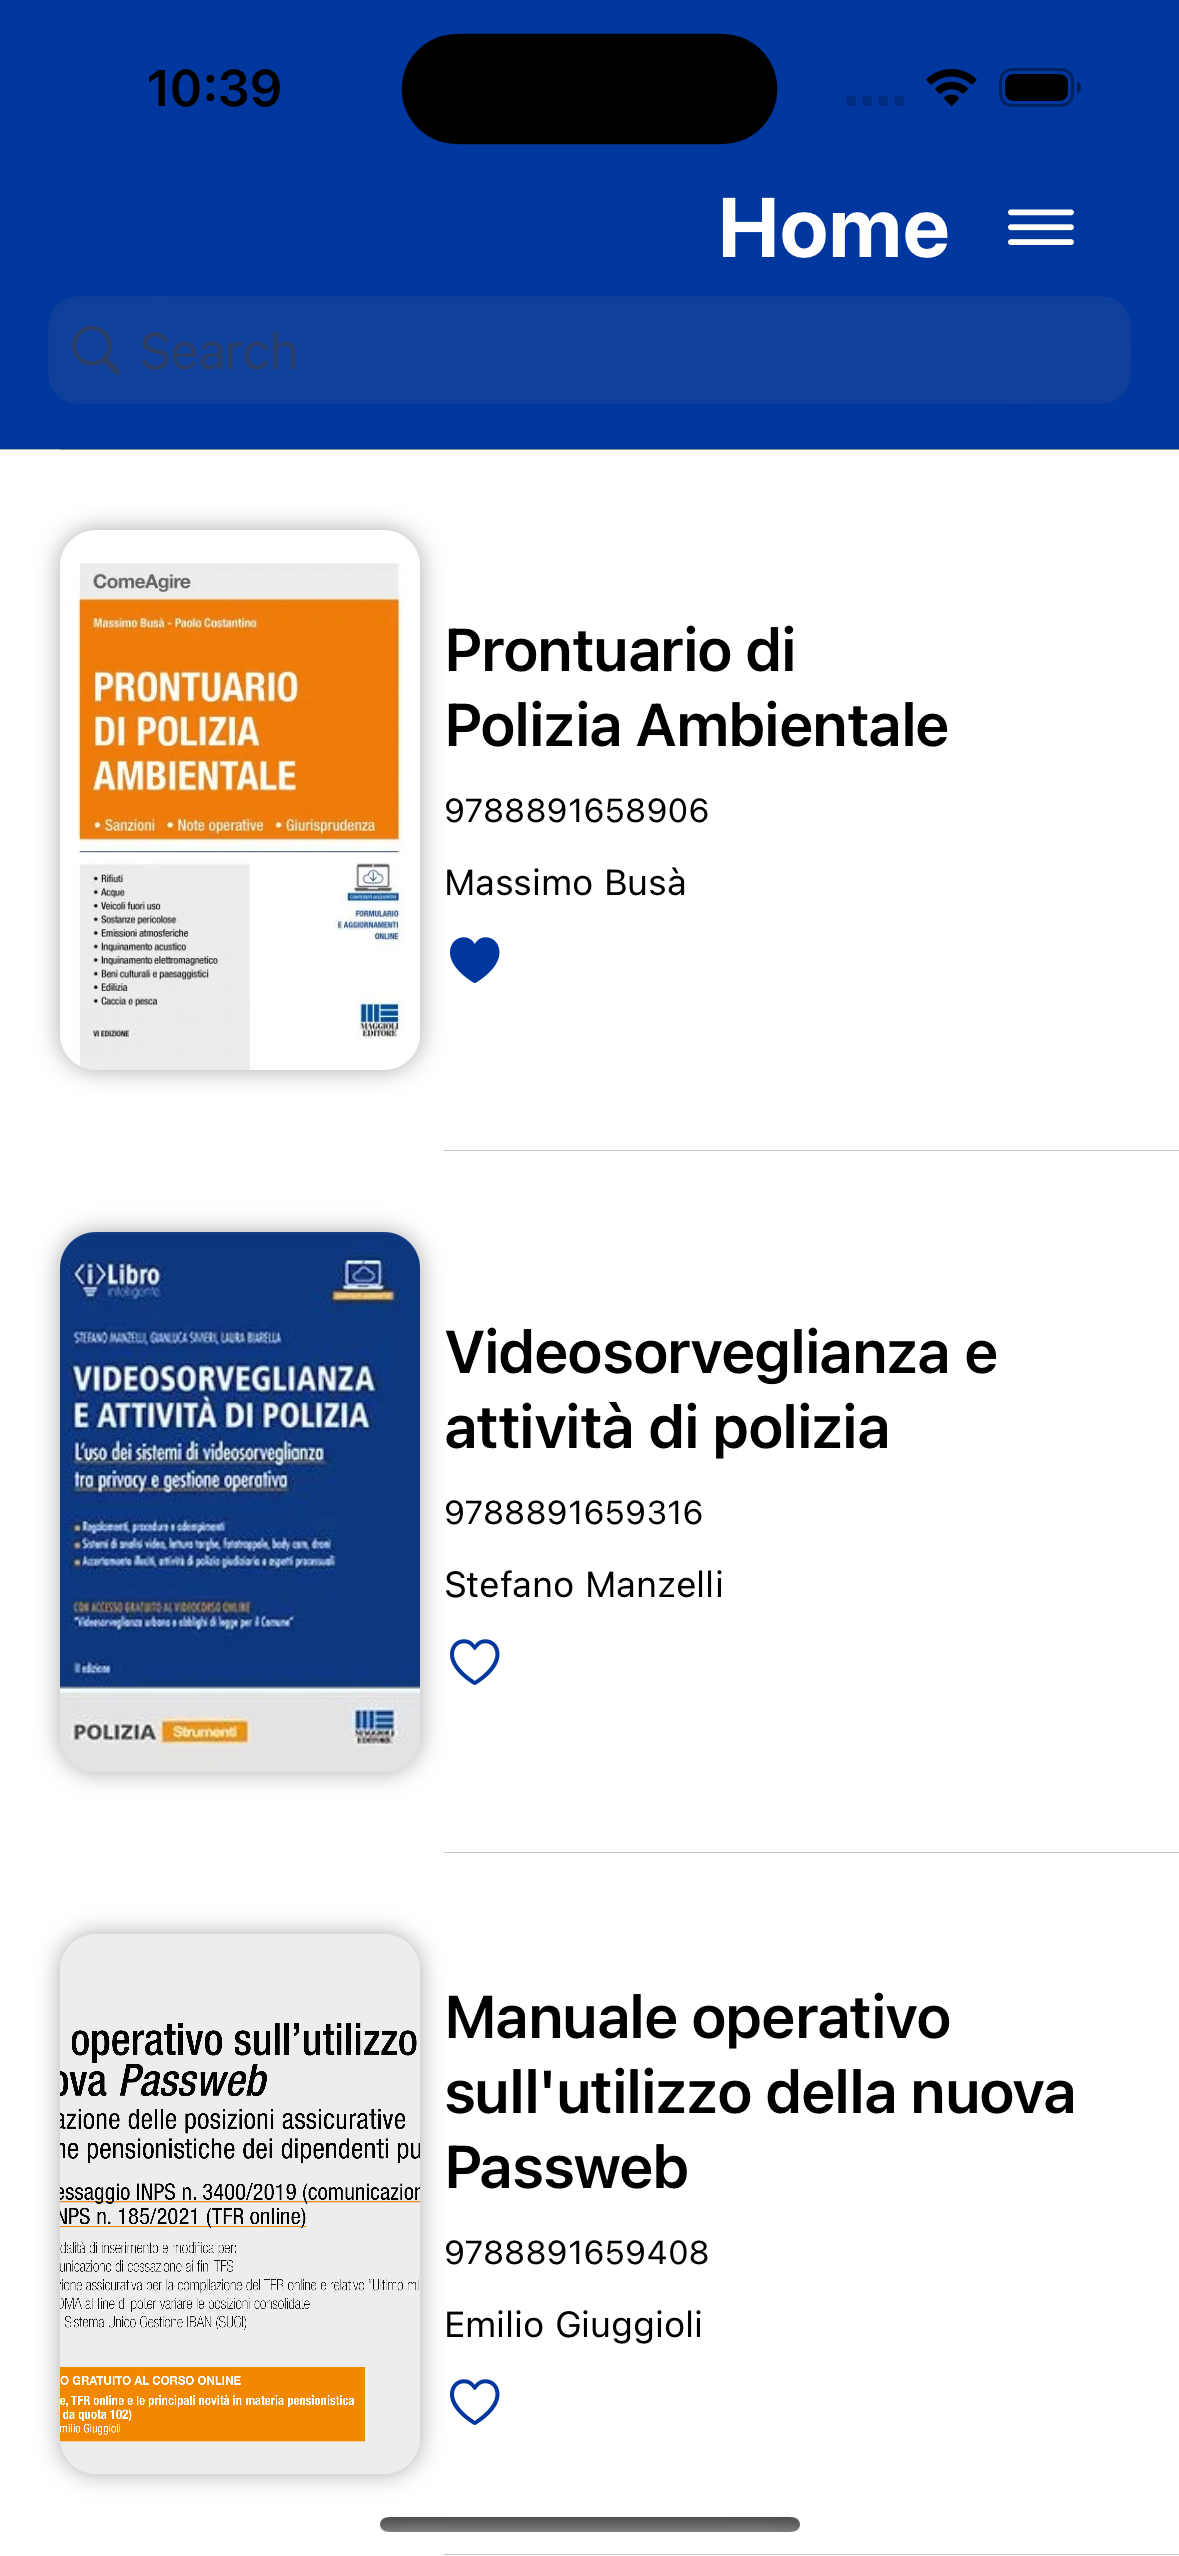
\includegraphics[width=0.21\textwidth]{img/Simulator Screen Shot - iPhone 14 Pro - 2022-10-05 at 10.39.58.png}
                \caption{Schermata home principale per la visualizzazione e la ricerca dei documenti digitali Maggioli}
                \label{homeios}
            \end{figure}
            
            \begin{figure}[H]
                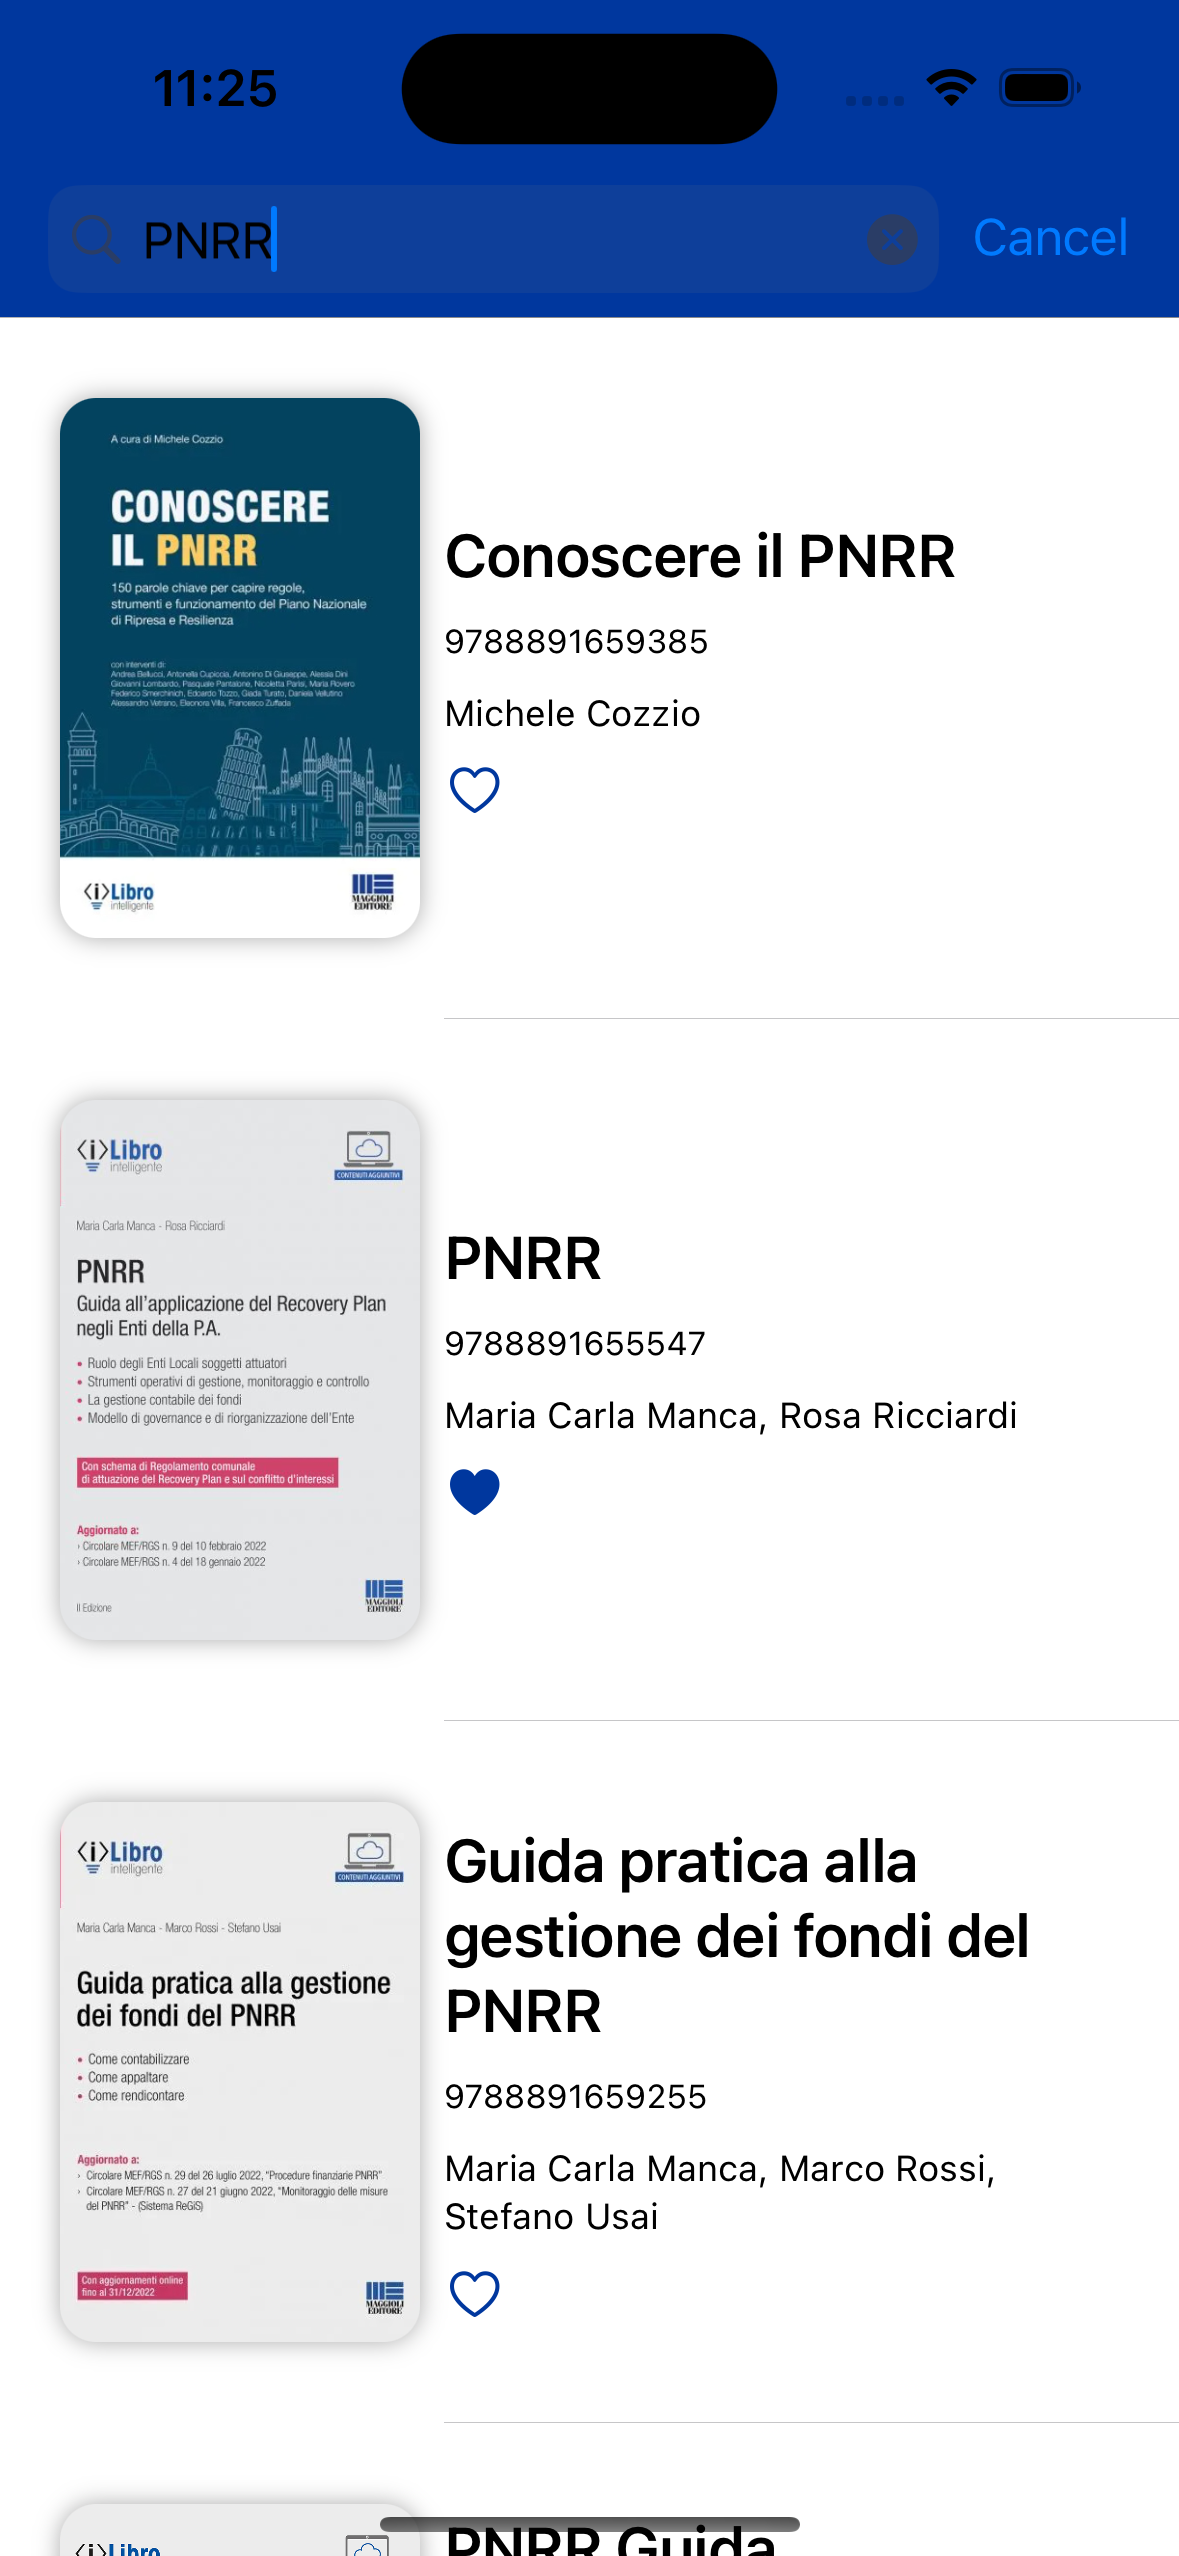
\includegraphics[width=0.21\textwidth]{img/Simulator Screen Shot - iPhone 14 Pro - 2022-10-05 at 11.25.21.png}
                \caption{Esempio di ricerca per parola chiave nella schermata principale}
                \label{ricercaios}
            \end{figure}

            \begin{figure}[H]
                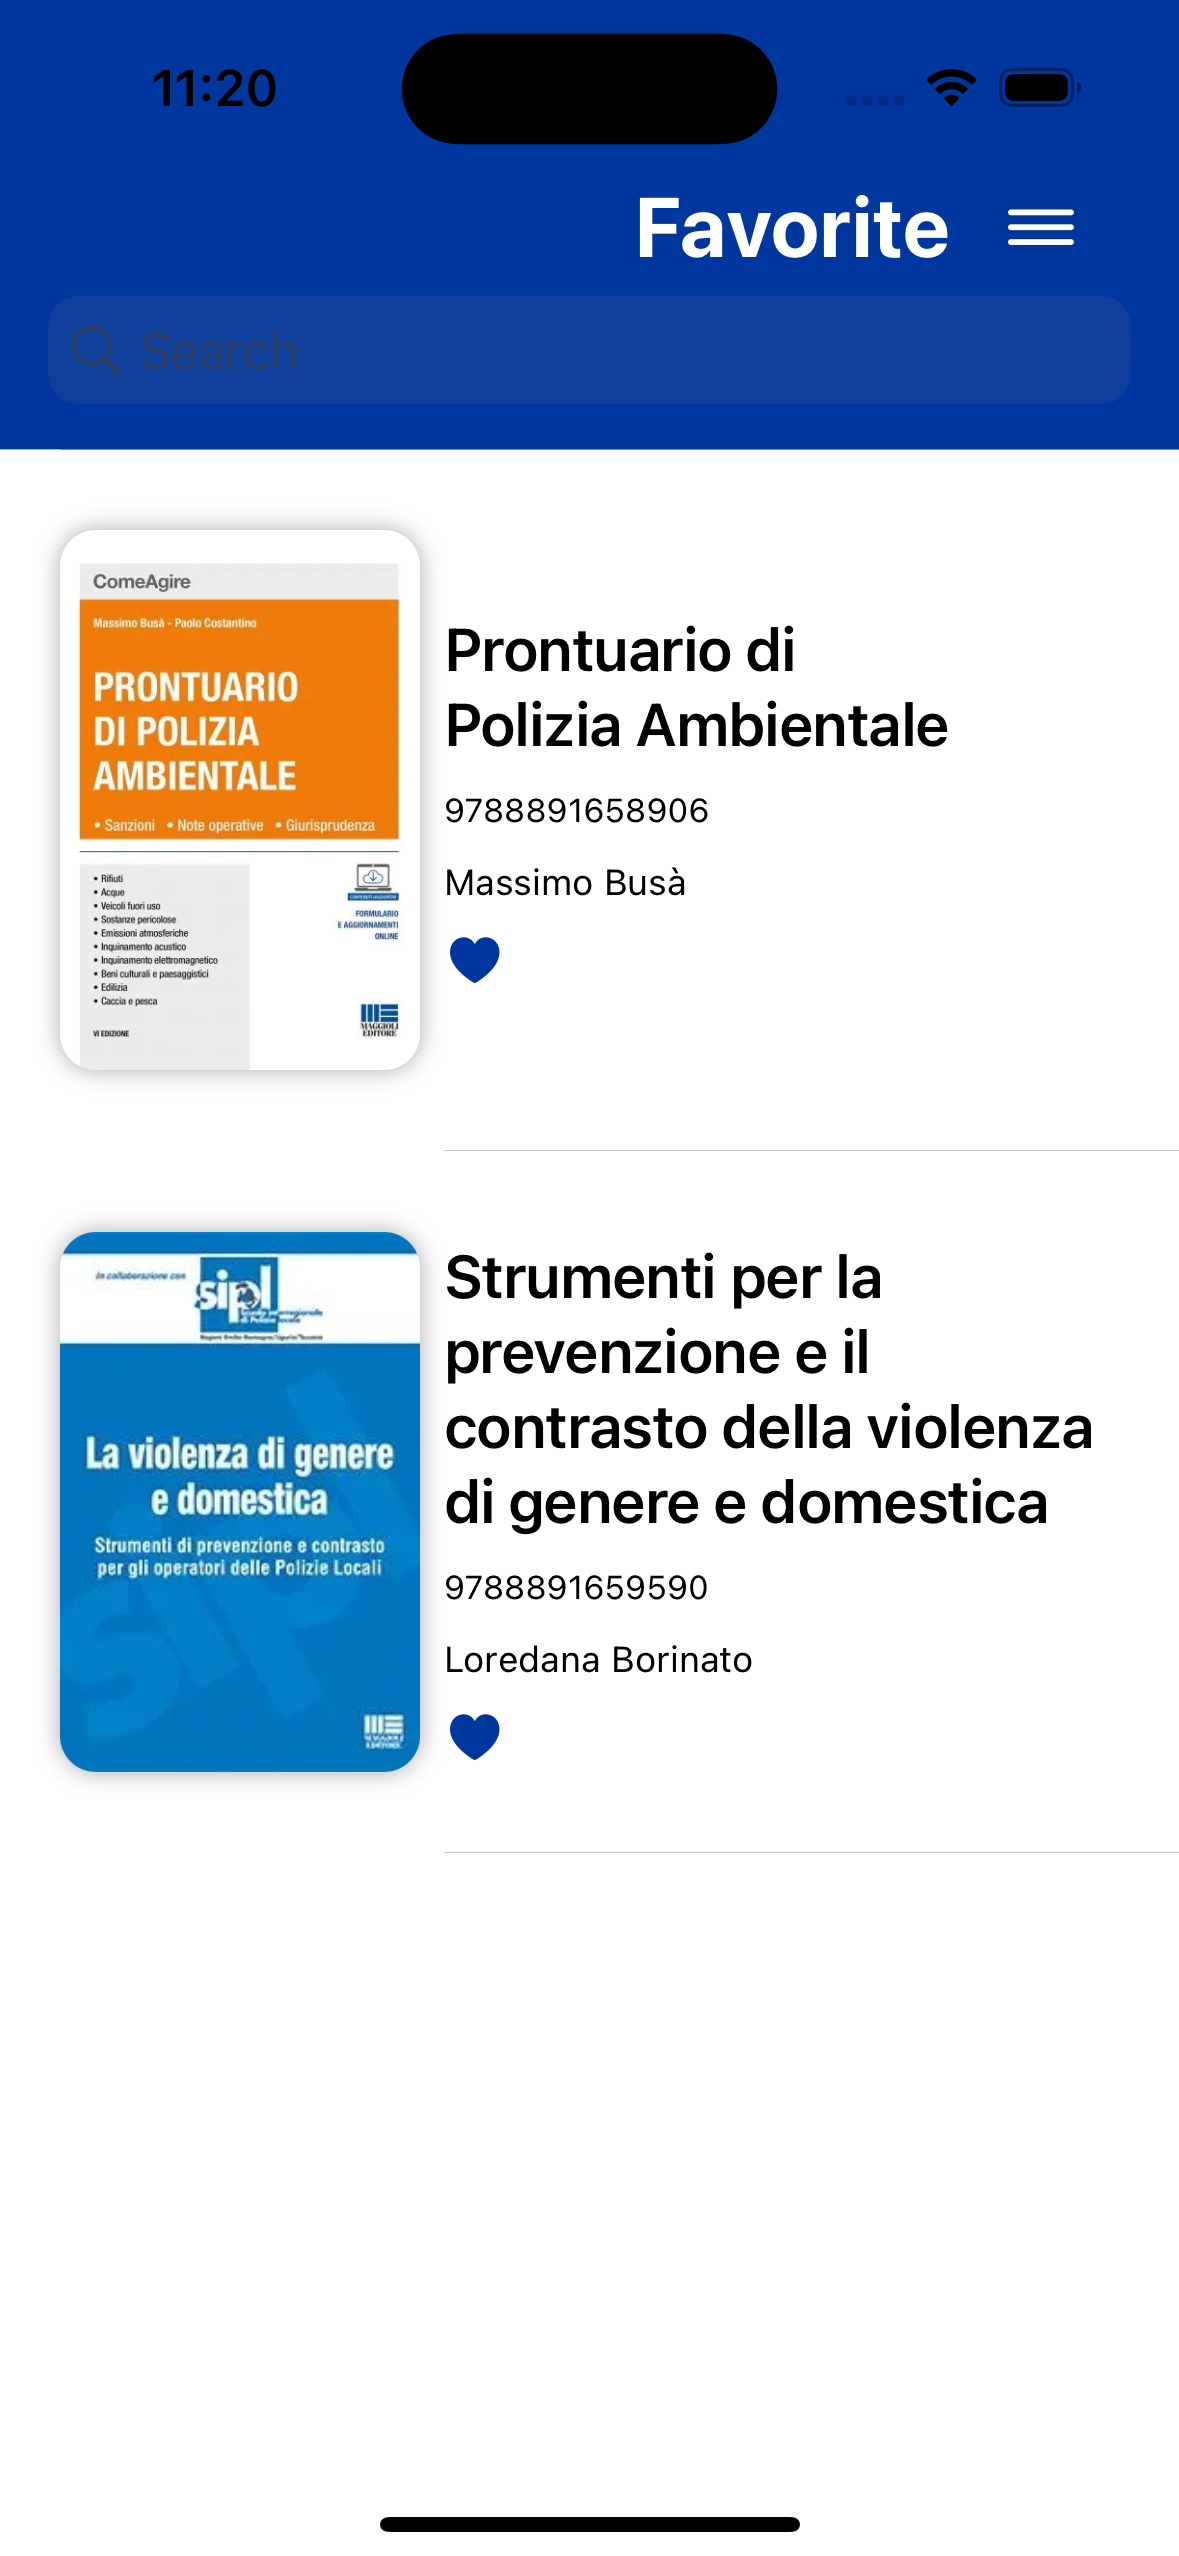
\includegraphics[width=0.21\textwidth]{img/Simulator Screen Shot - iPhone 14 Pro - 2022-10-05 at 11.20.04.png}
                \caption{Schermata per la visualizzazione e la ricerca dei documenti preferiti dall'utente}
                \label{preferitiios}
            \end{figure}

            \begin{figure}[H]
                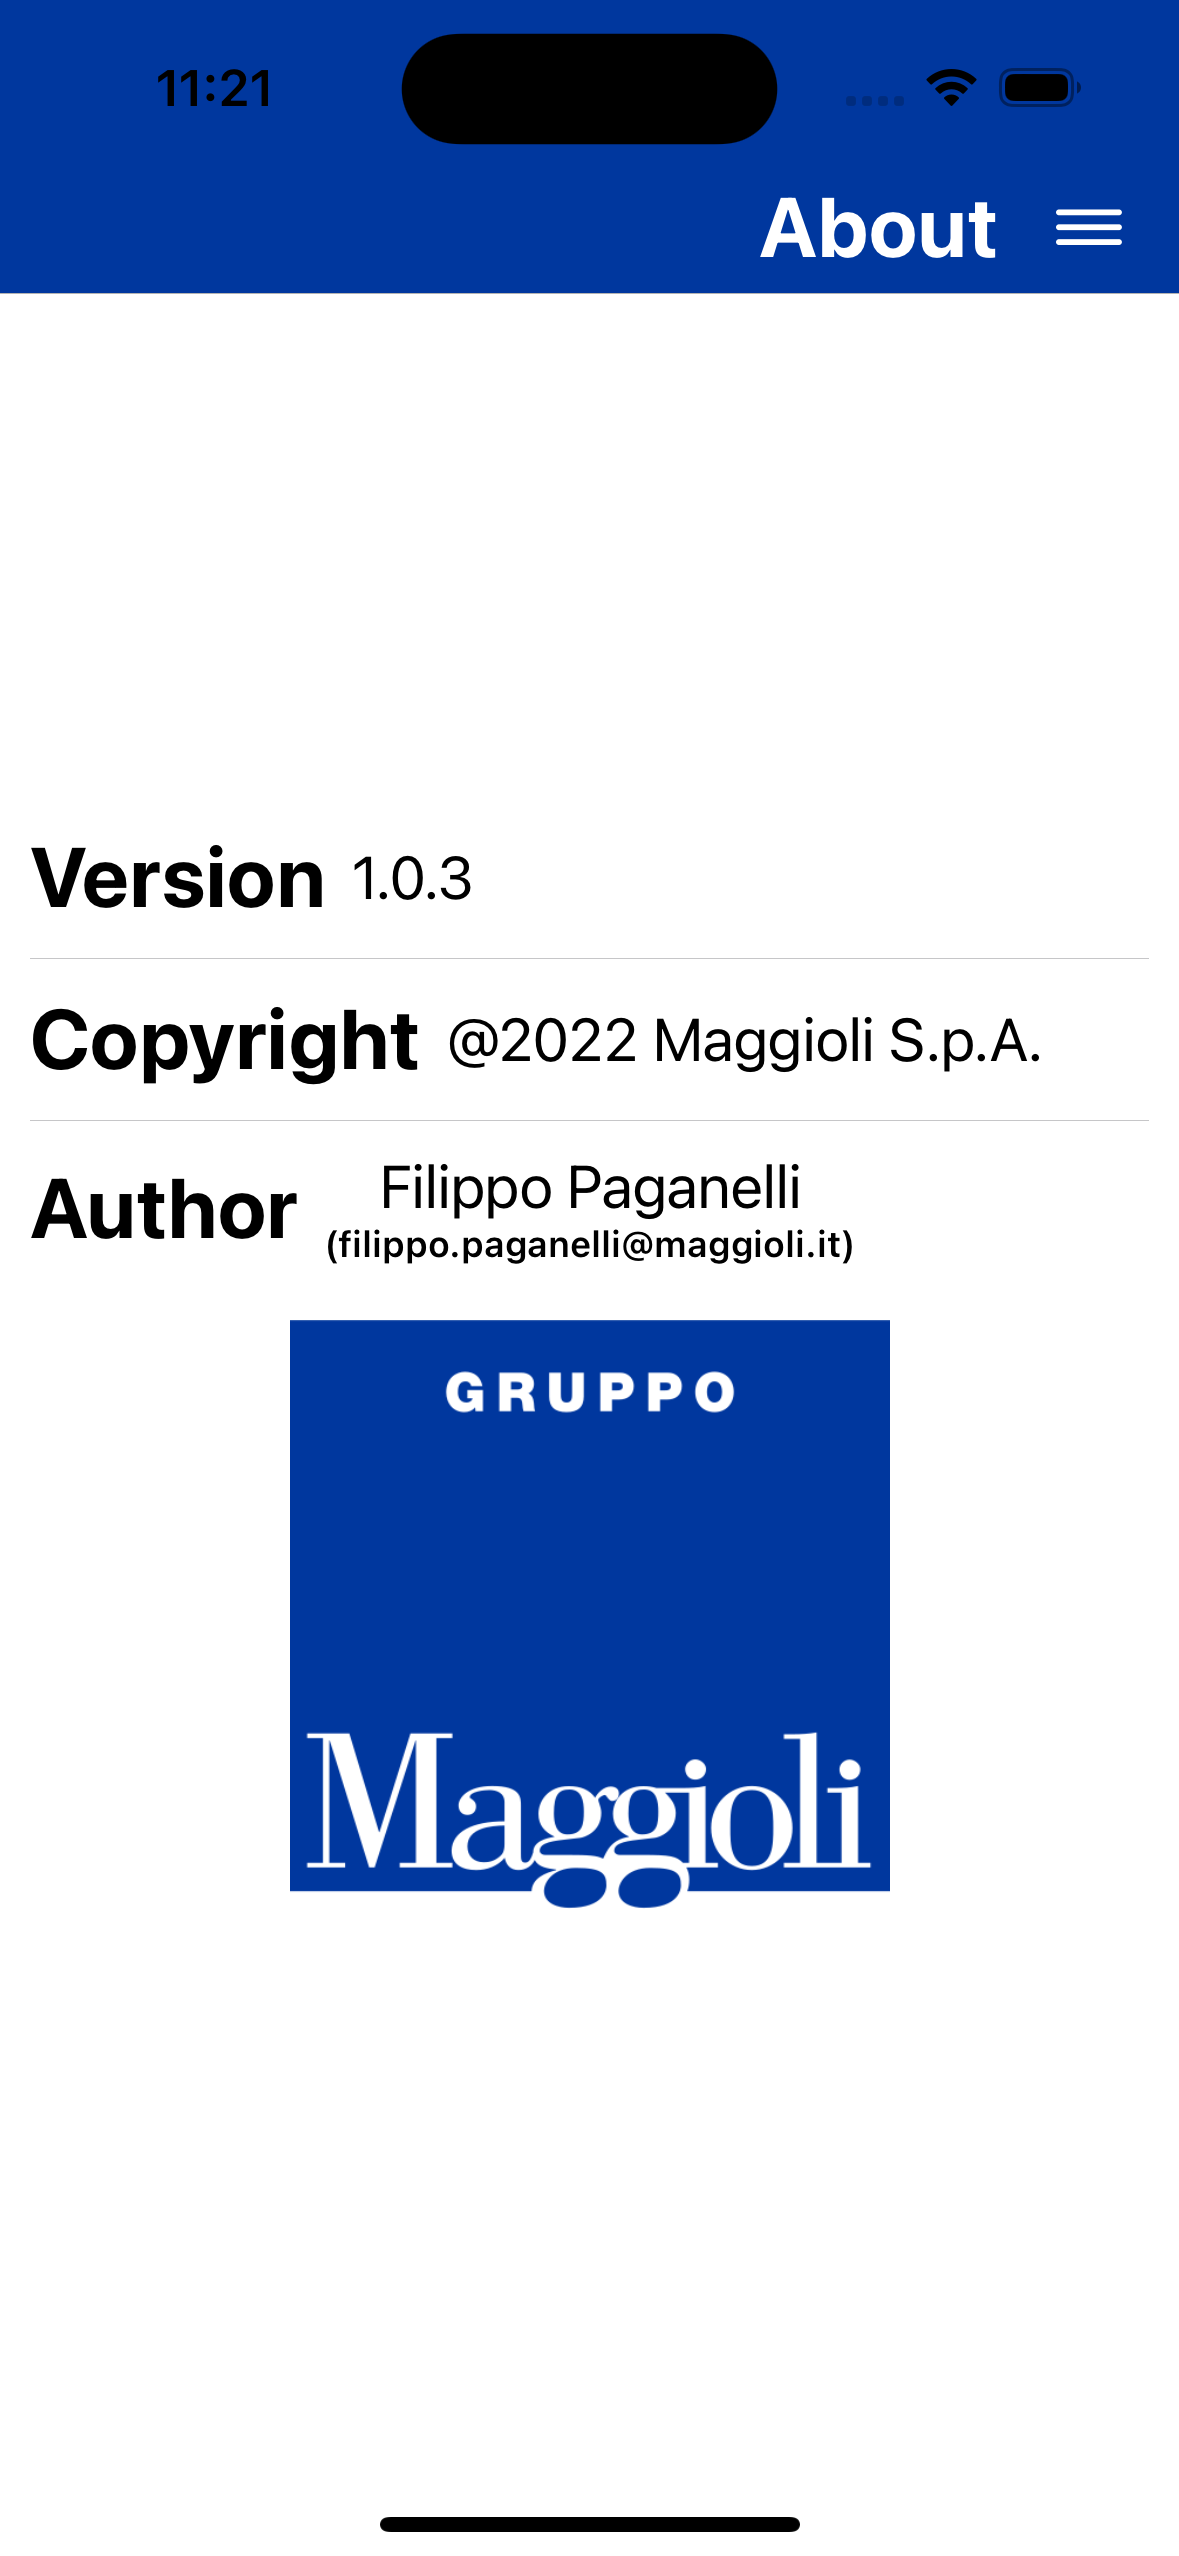
\includegraphics[width=0.21\textwidth]{img/Simulator Screen Shot - iPhone 14 Pro - 2022-10-05 at 11.21.25.png}
                \caption{Schermata per la visualizzazione delle informazioni generali relative alla applicazione}
                \label{aboutios}
            \end{figure}

\begin{comment}
            \begin{figure}[H]
                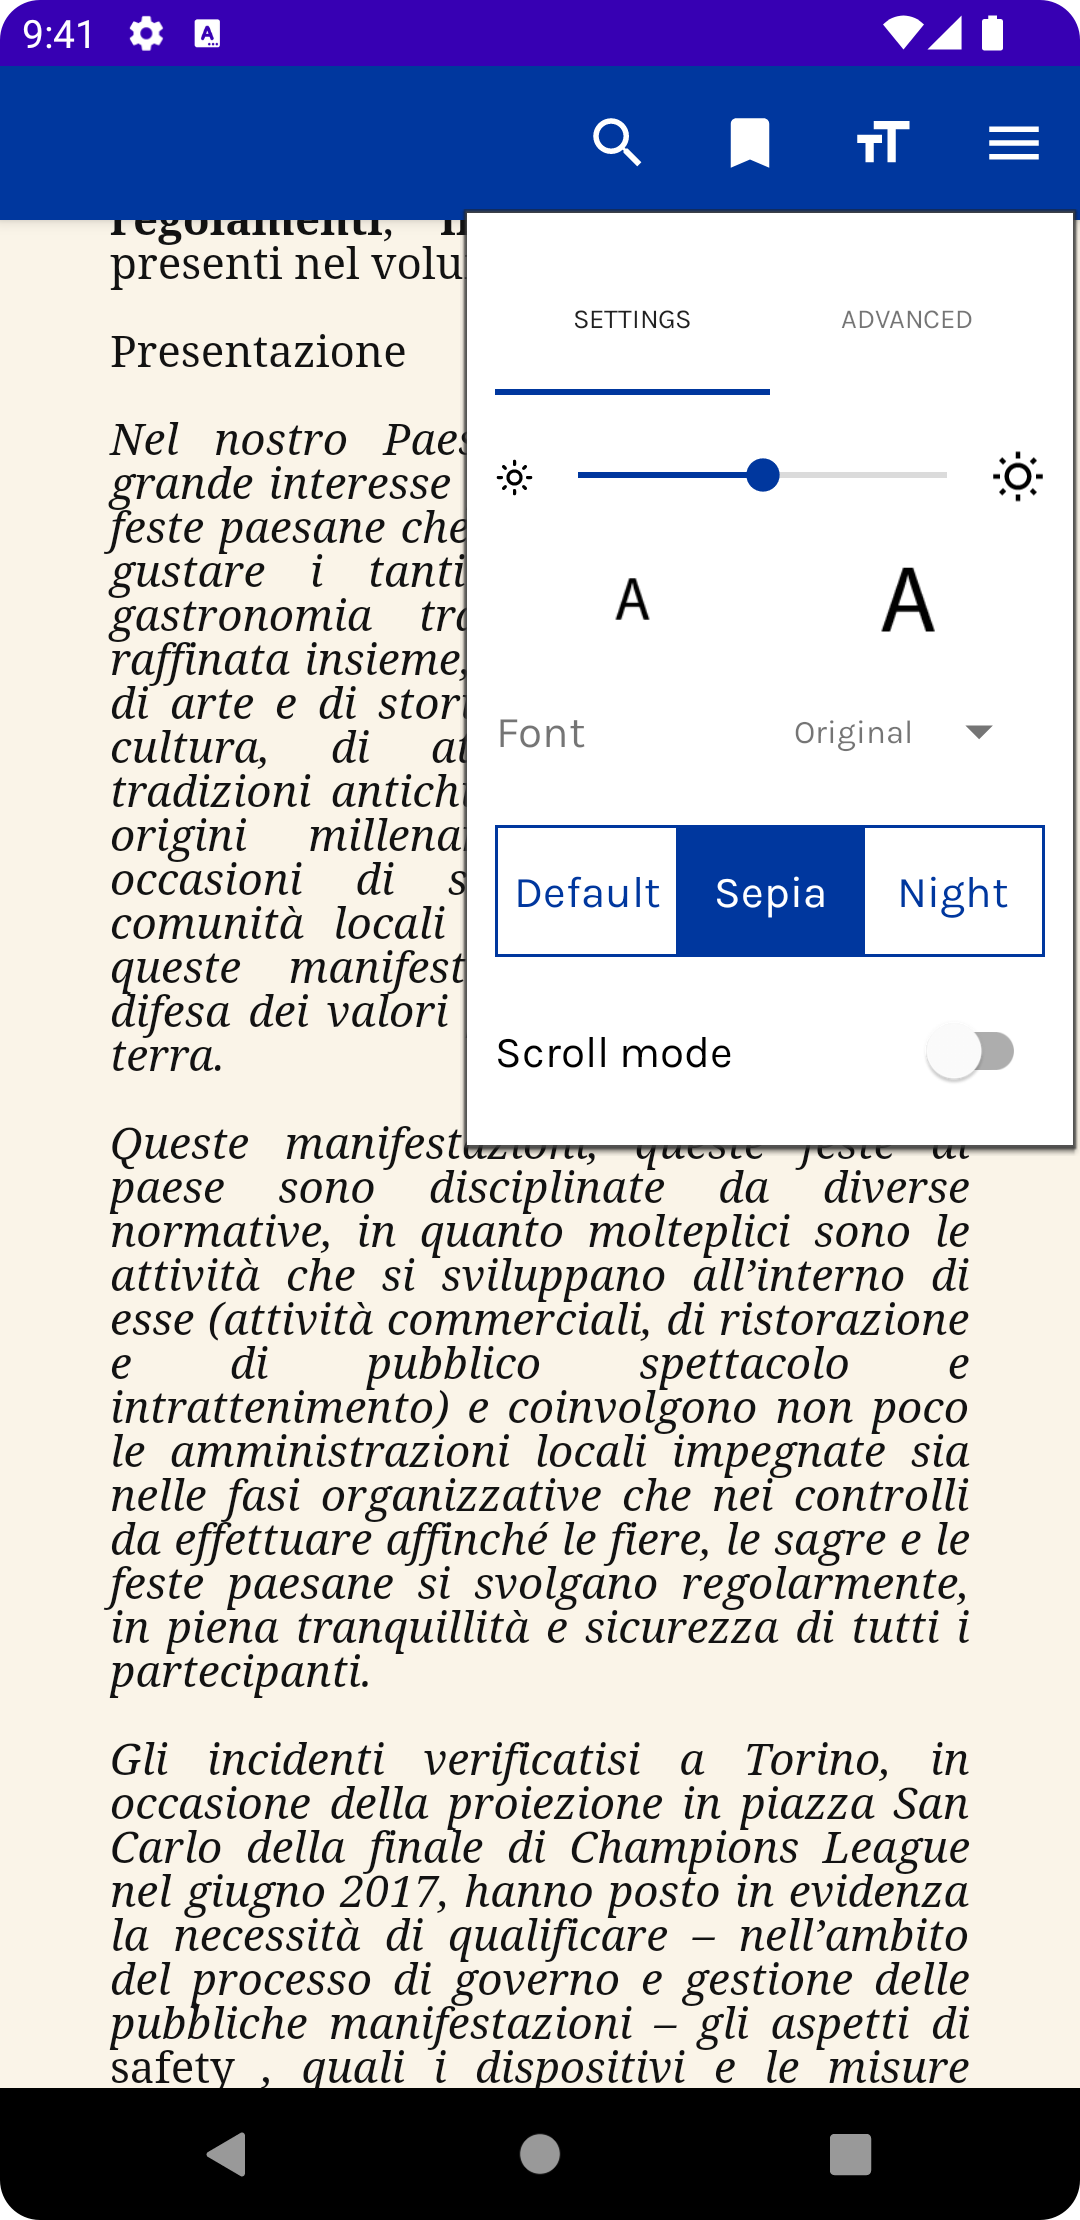
\includegraphics[width=0.21\textwidth]{img/reader_settings.png.todo}
                \caption{Lettura documento digitale d'esempio e impostazioni del lettore}
                \label{readersettings}
            \end{figure}
            
            \begin{figure}[H]
                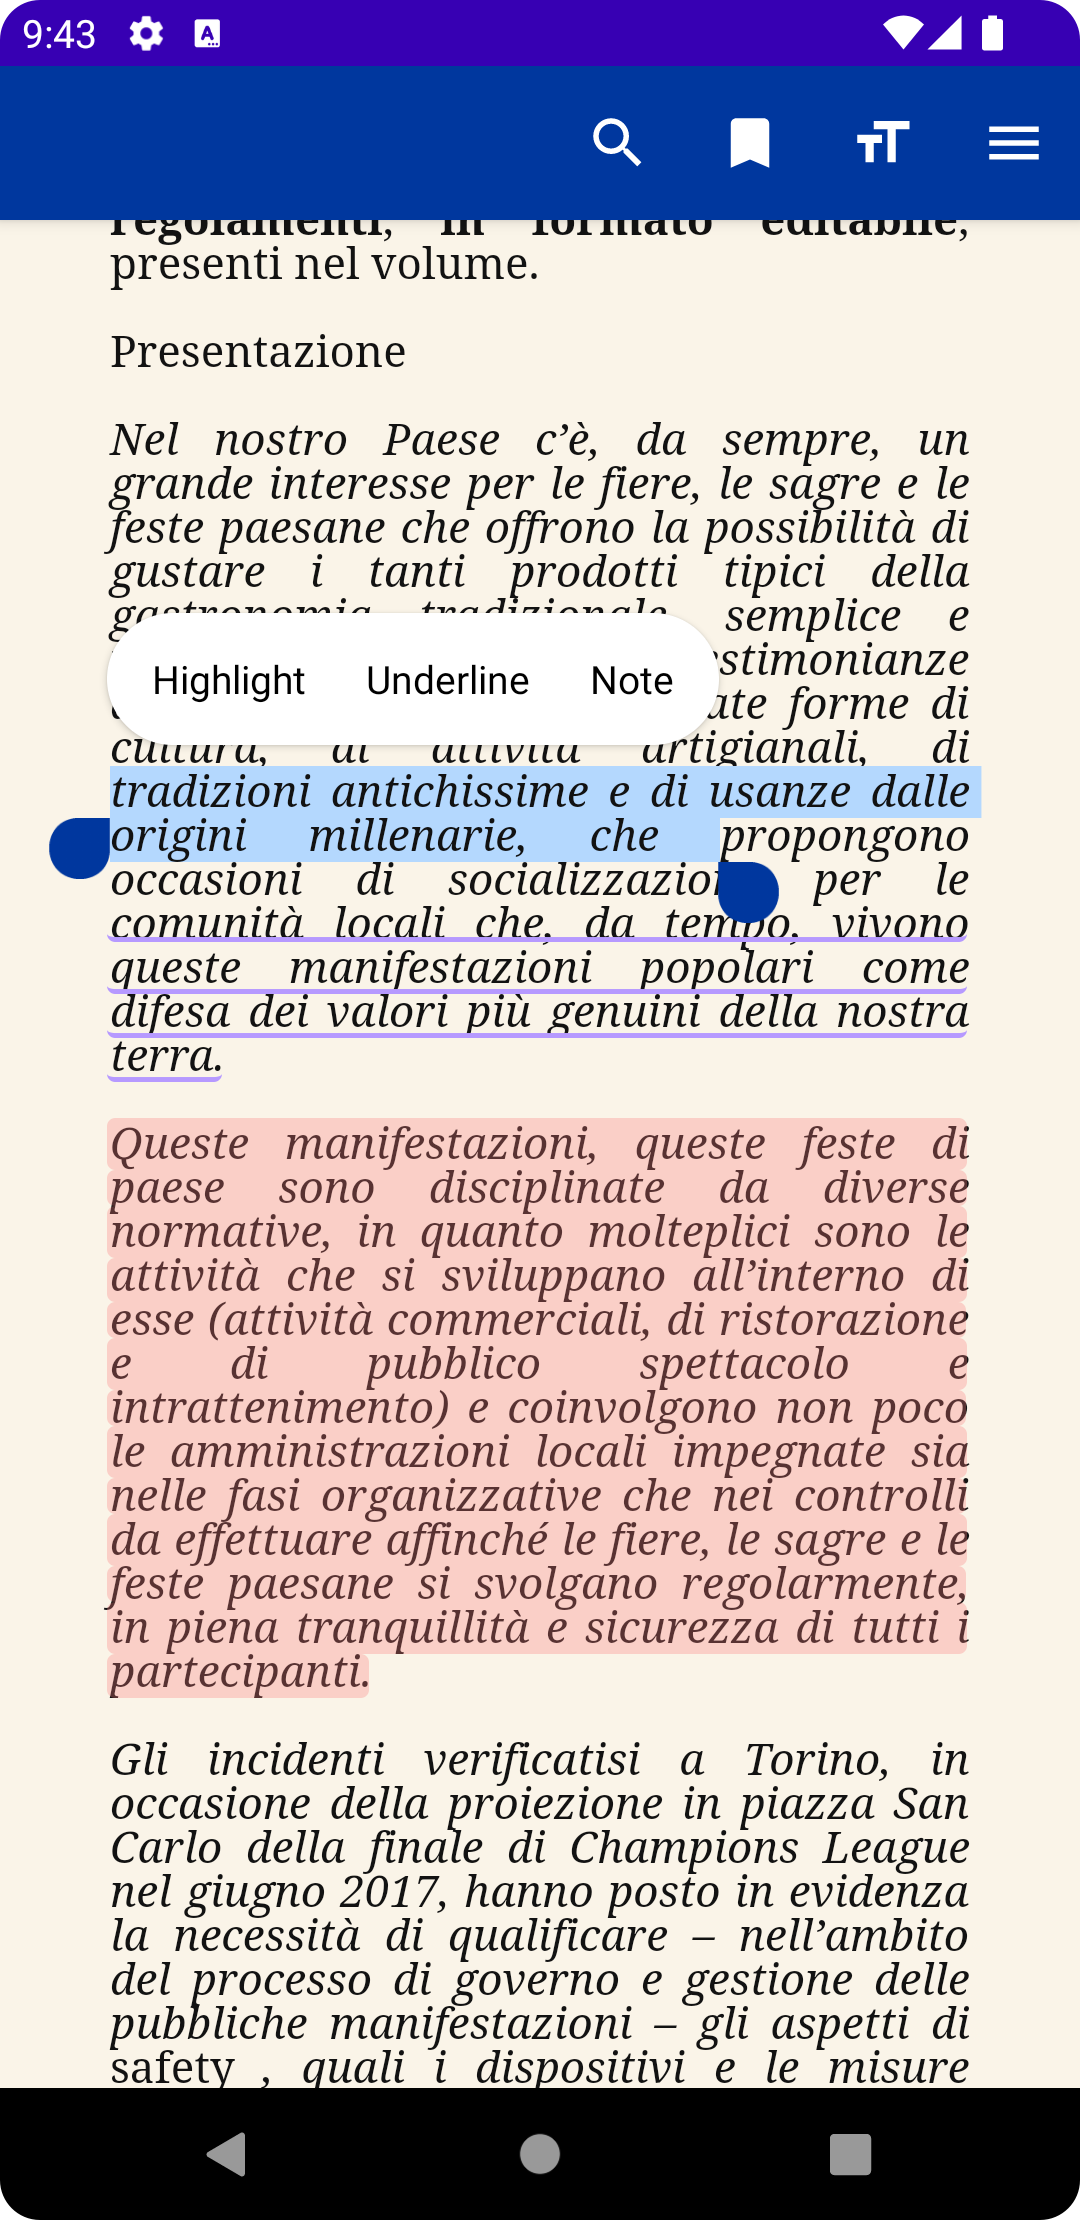
\includegraphics[width=0.21\textwidth]{img/annotations.png}
                \caption{Esempio di inserimento di annotazioni come evidenziazioni e sottolineature}
                \label{annotations}
            \end{figure}
            
            \begin{figure}[H]
                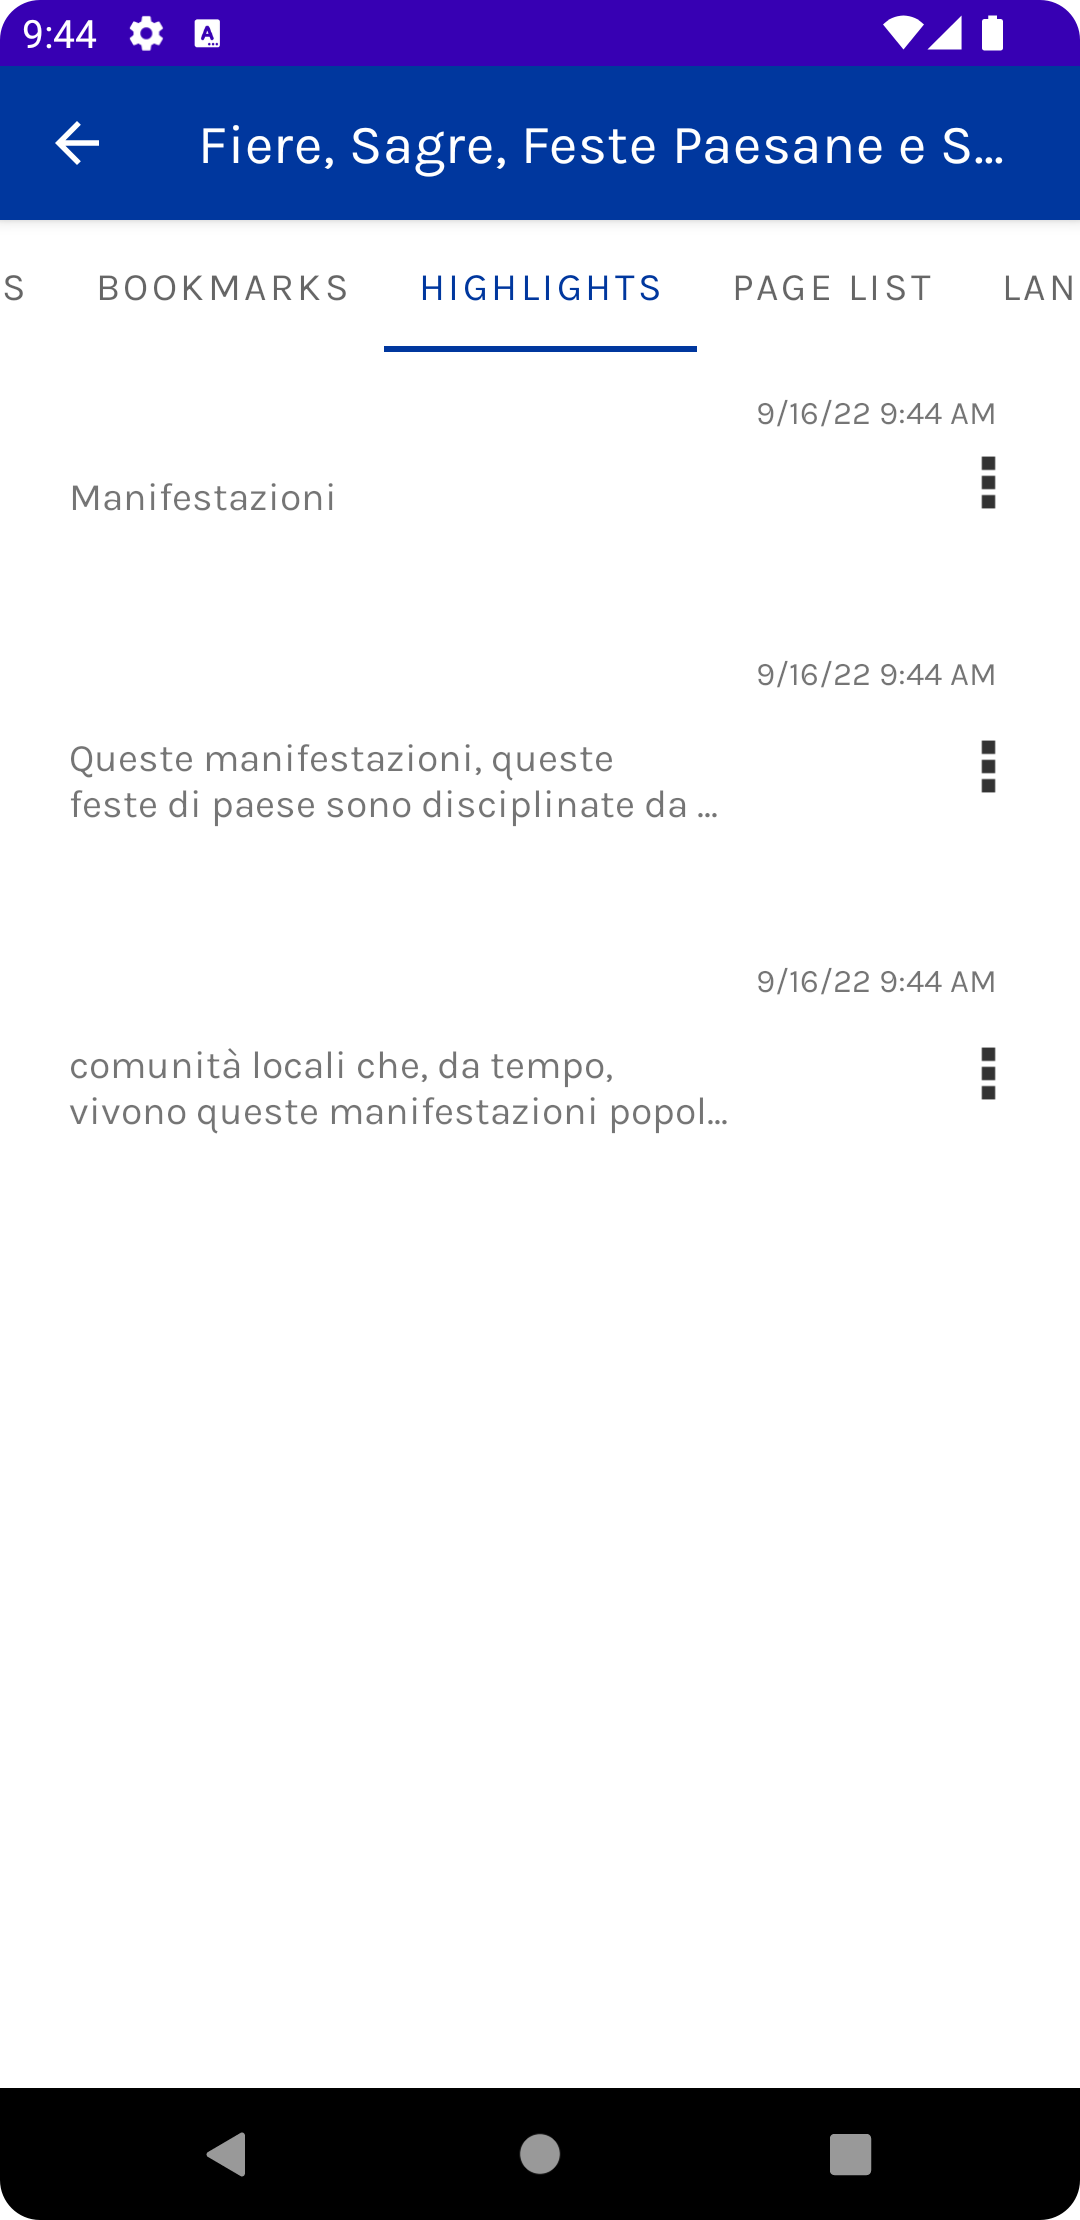
\includegraphics[width=0.21\textwidth]{img/annotation2.png}
                \caption{Annotazioni memorizzate sul dispositivo e consultabili dal menu del lettore}
                \label{annotation2}
            \end{figure}

            \begin{figure}[H]
                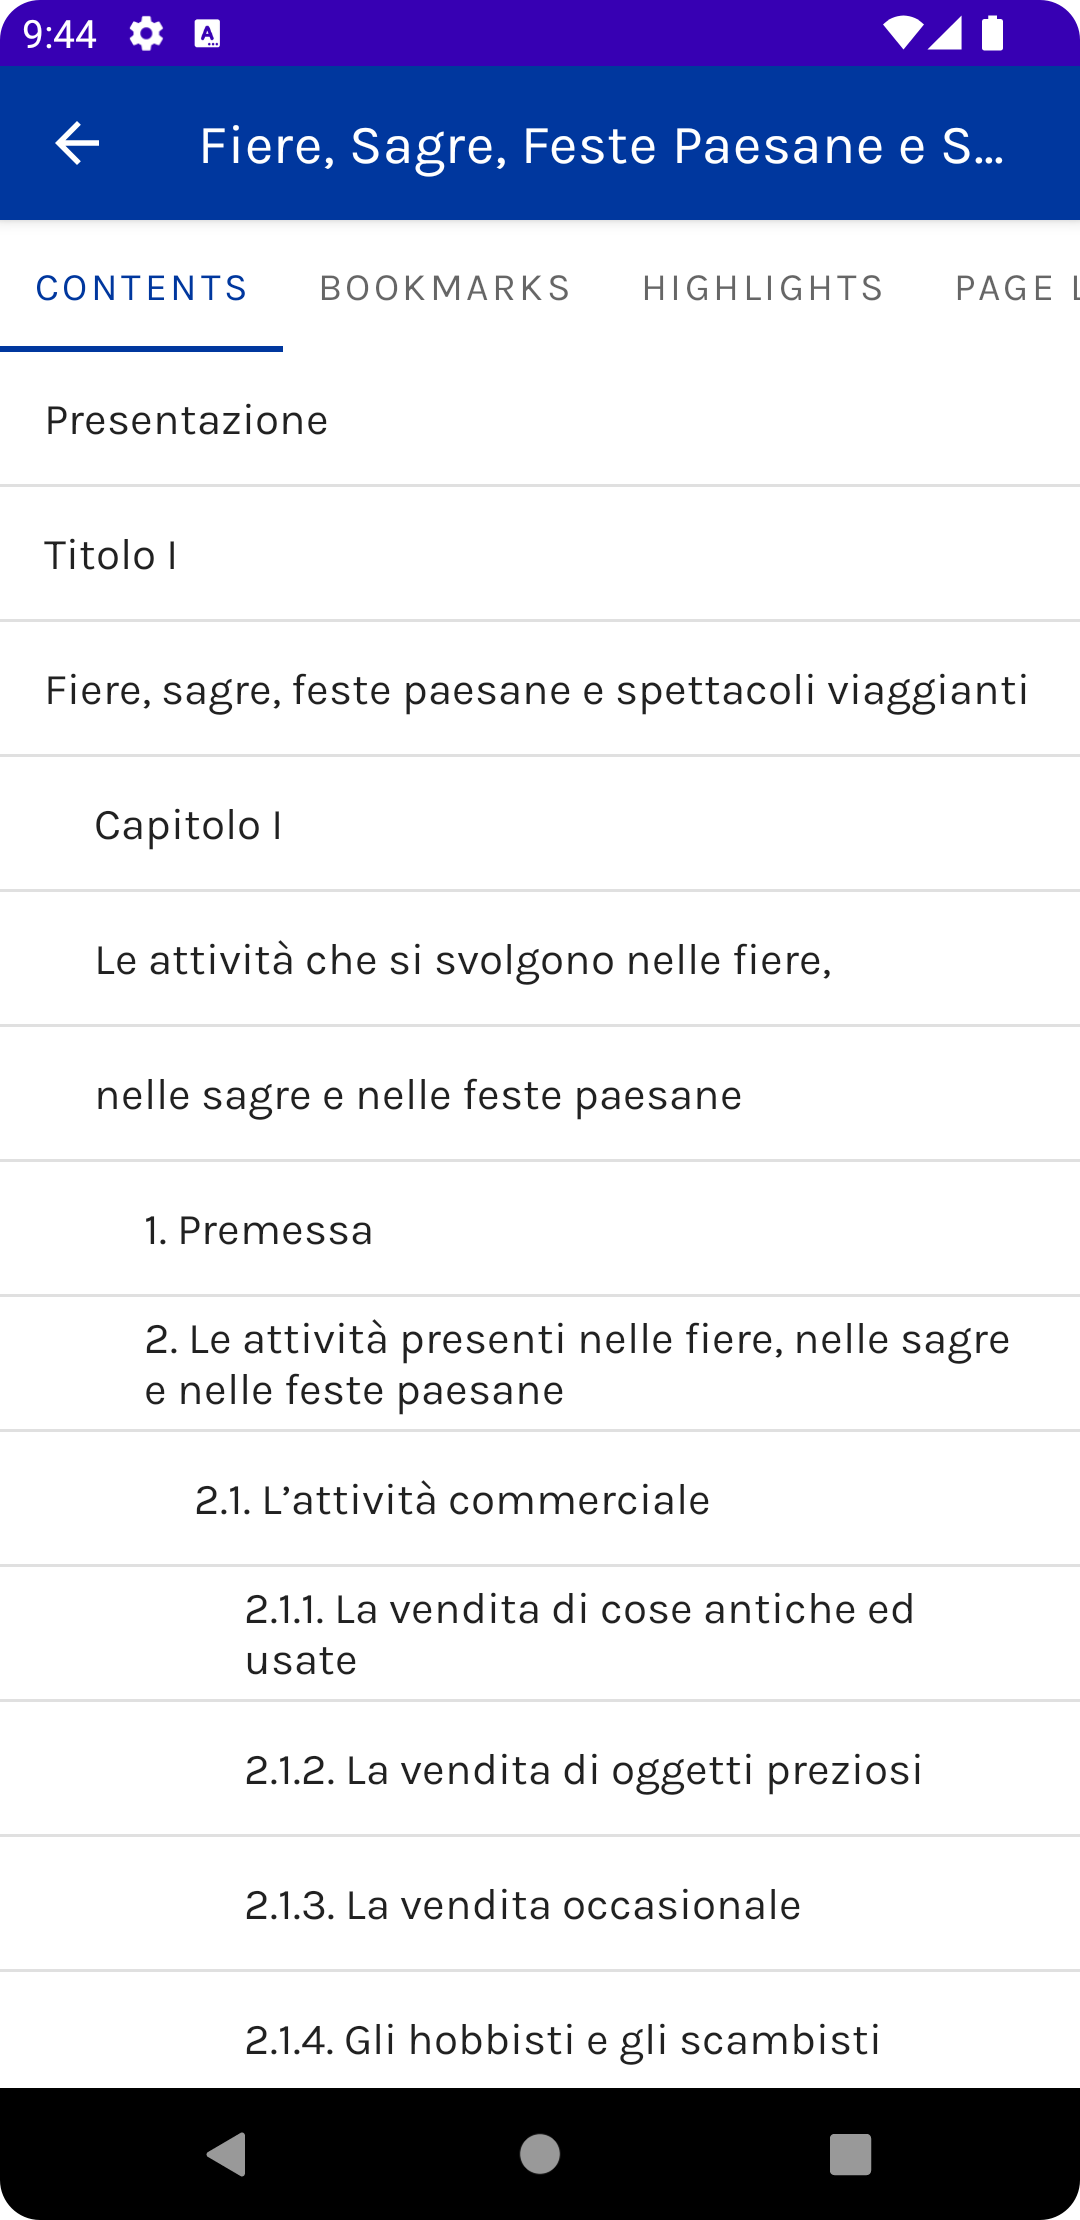
\includegraphics[width=0.21\textwidth]{img/toc.png}
                \caption{Elenco dei contenuti (TOC) del documento aperto e consultabile dal menu del lettore}
                \label{toc}
            \end{figure}
            
            \begin{figure}[H]
                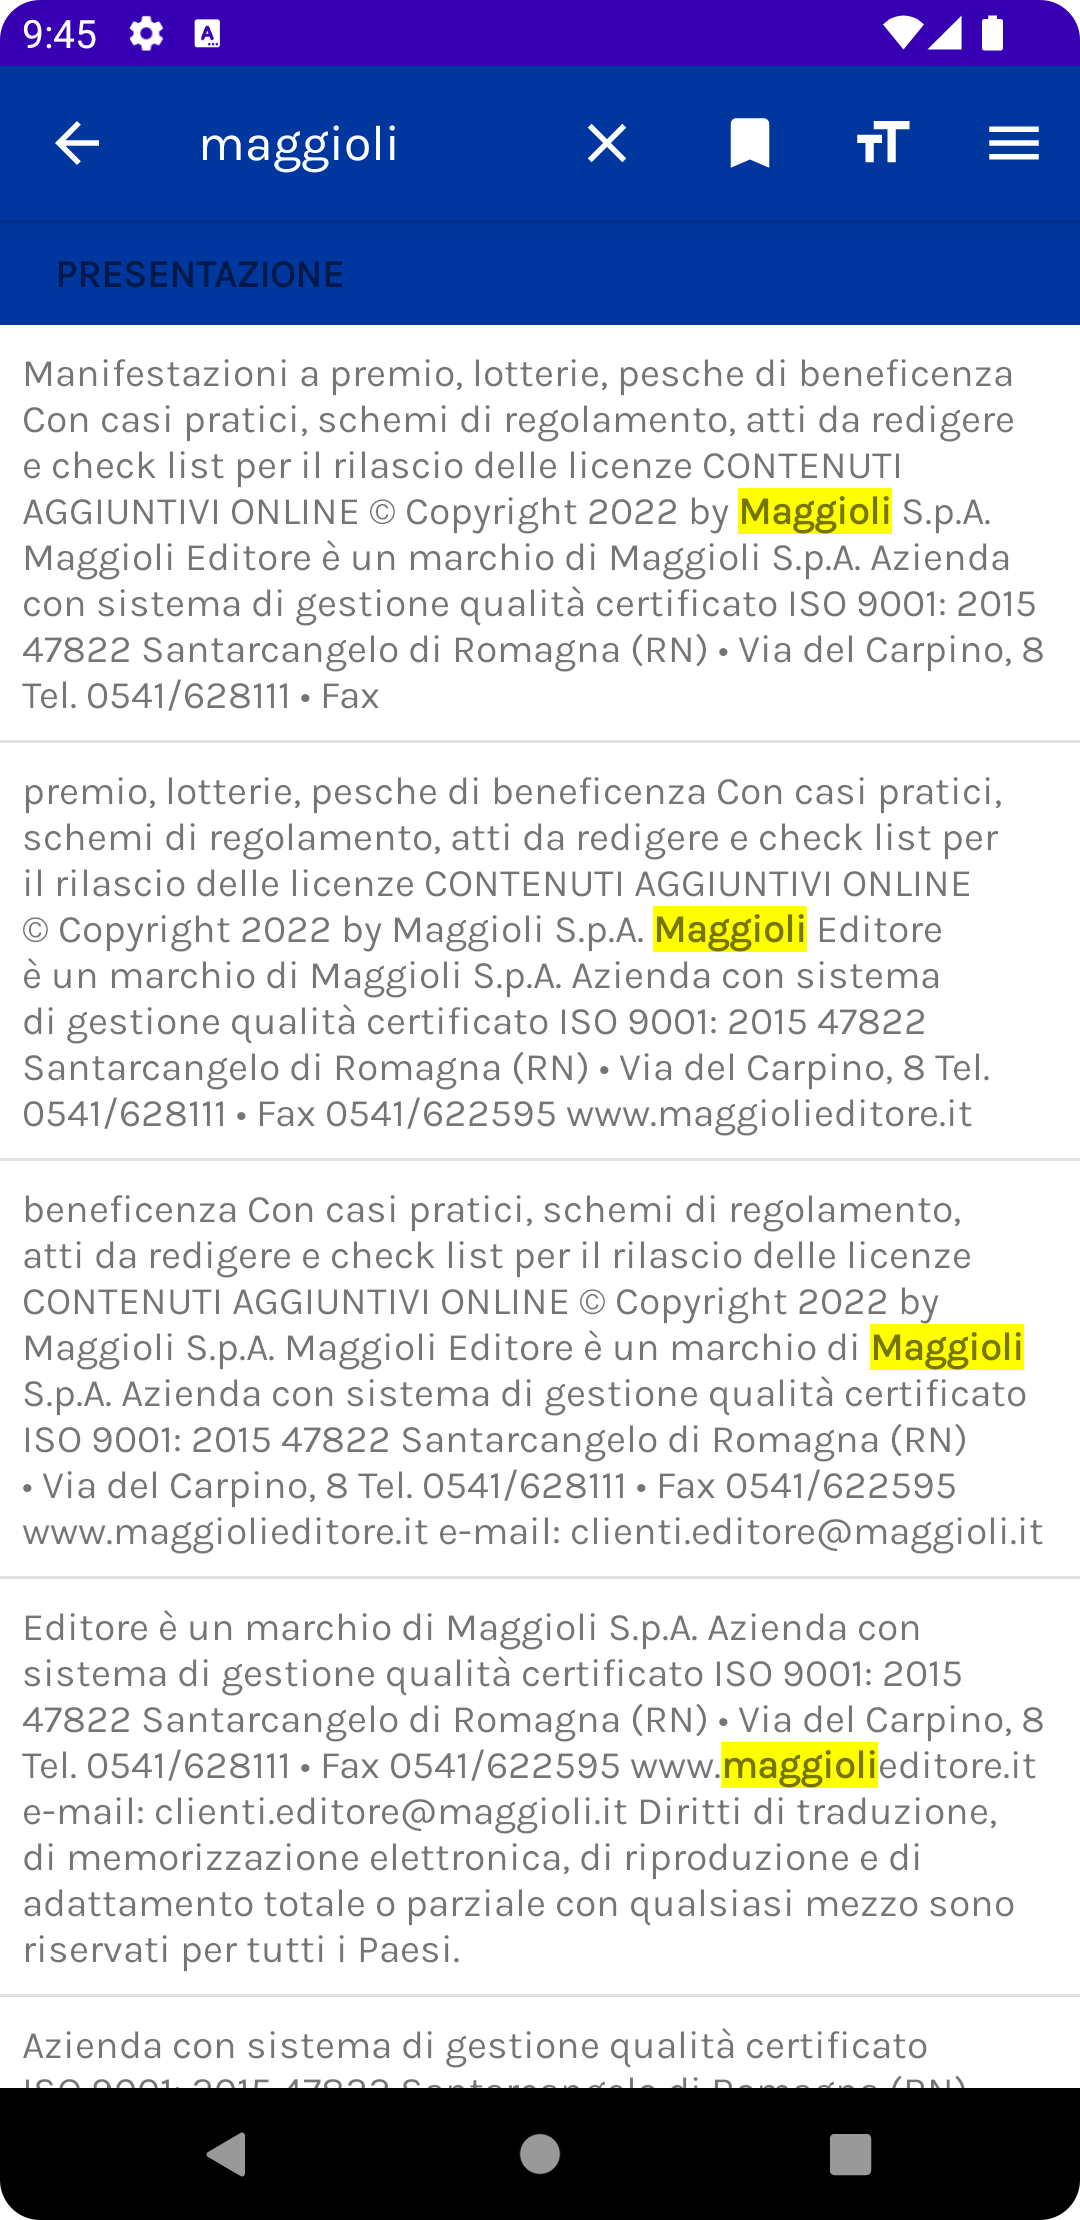
\includegraphics[width=0.21\textwidth]{img/ricerca_testo.png}
                \caption{Ricerca testuale nel contenuto del documento aperto con relativo risultato}
                \label{ricerca_testo}
            \end{figure}
            
            \begin{figure}[H]
                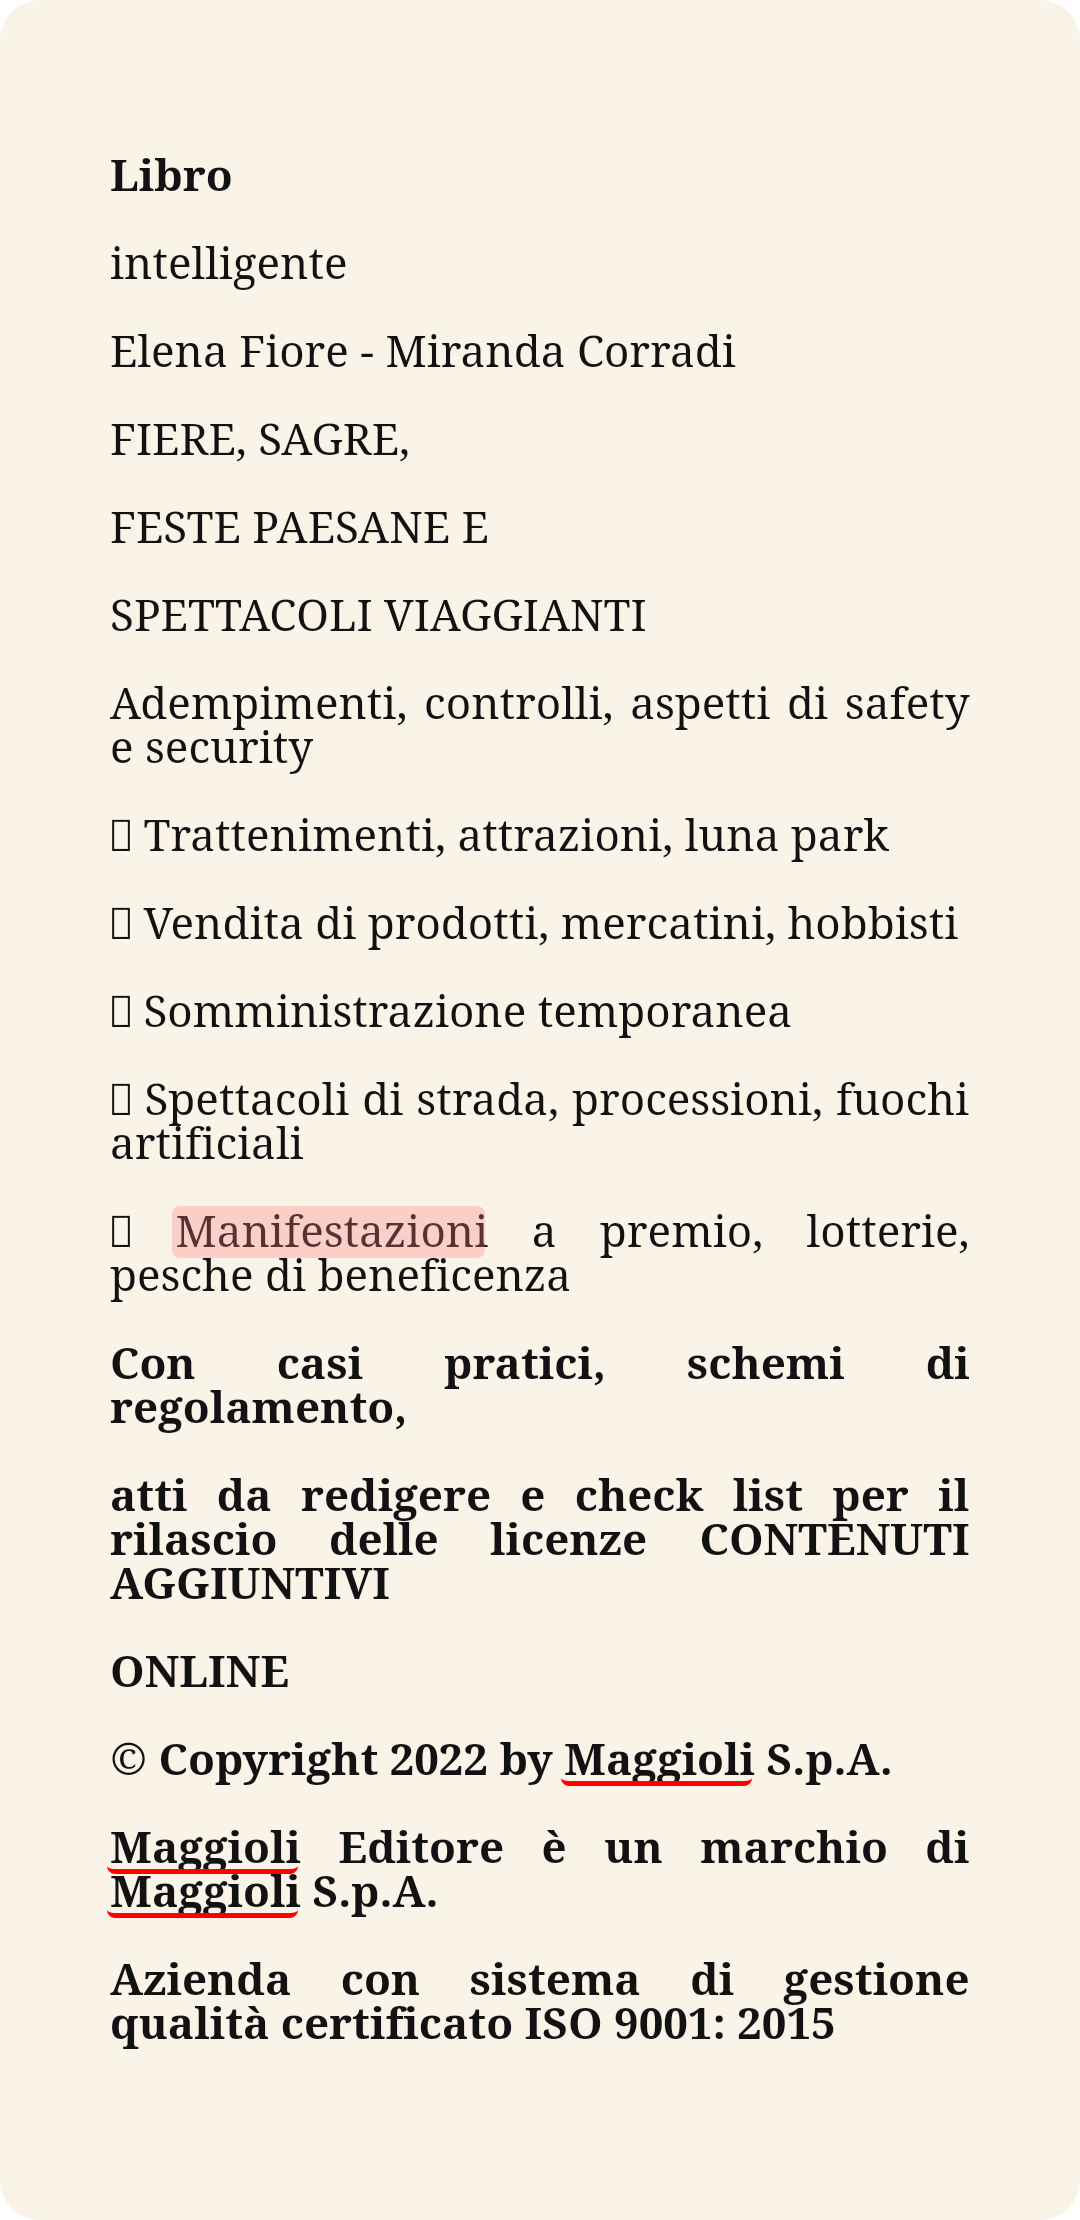
\includegraphics[width=0.21\textwidth]{img/ricerca_testo2.png}
                \caption{Evidenziazioni automatiche delle occorrenze del testo cercato}
                \label{ricerca_testo2}
            \end{figure}
\end{comment}
\end{multicols}

\subsection{Continuous Integration}
Nelle seguenti schermate ottenute dalla piattaforma GitLab viene mostrato l'effettivo utilizzo delle tecniche di Continuous Integration come descritto nel capitolo \ref{ch:ch4}. Nella schermata \ref{pipelinesapp} sono raffigurate alcune delle ultime pipeline eseguite per l'applicazione realizzata: due pipeline di aggiornamento delle dipendenze automatico fallite a causa di errori durante i test e due pipeline per il rilascio alpha e beta terminate con successo.

\begin{figure}[H]
\centering
    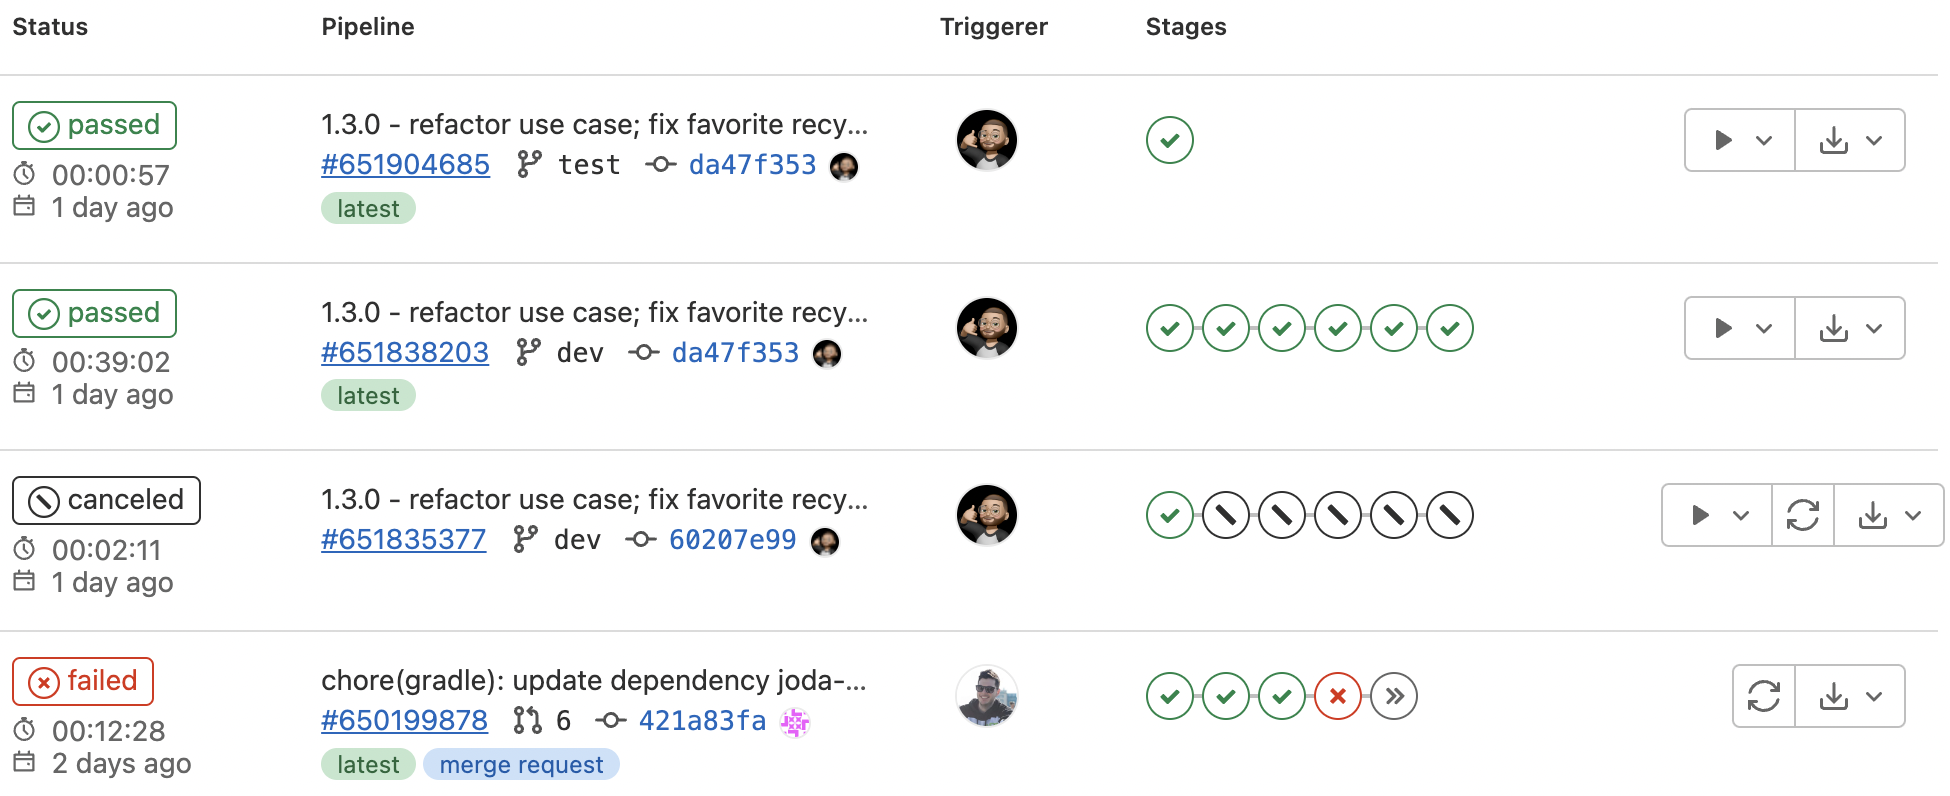
\includegraphics[width=1\textwidth]{img/Screenshot 2022-09-28 at 15.58.43.png}
    \caption{Schermata GitLab - Ultime pipeline eseguite.}
    \label{pipelinesapp}
\end{figure}

\begin{figure}[H]
\centering
    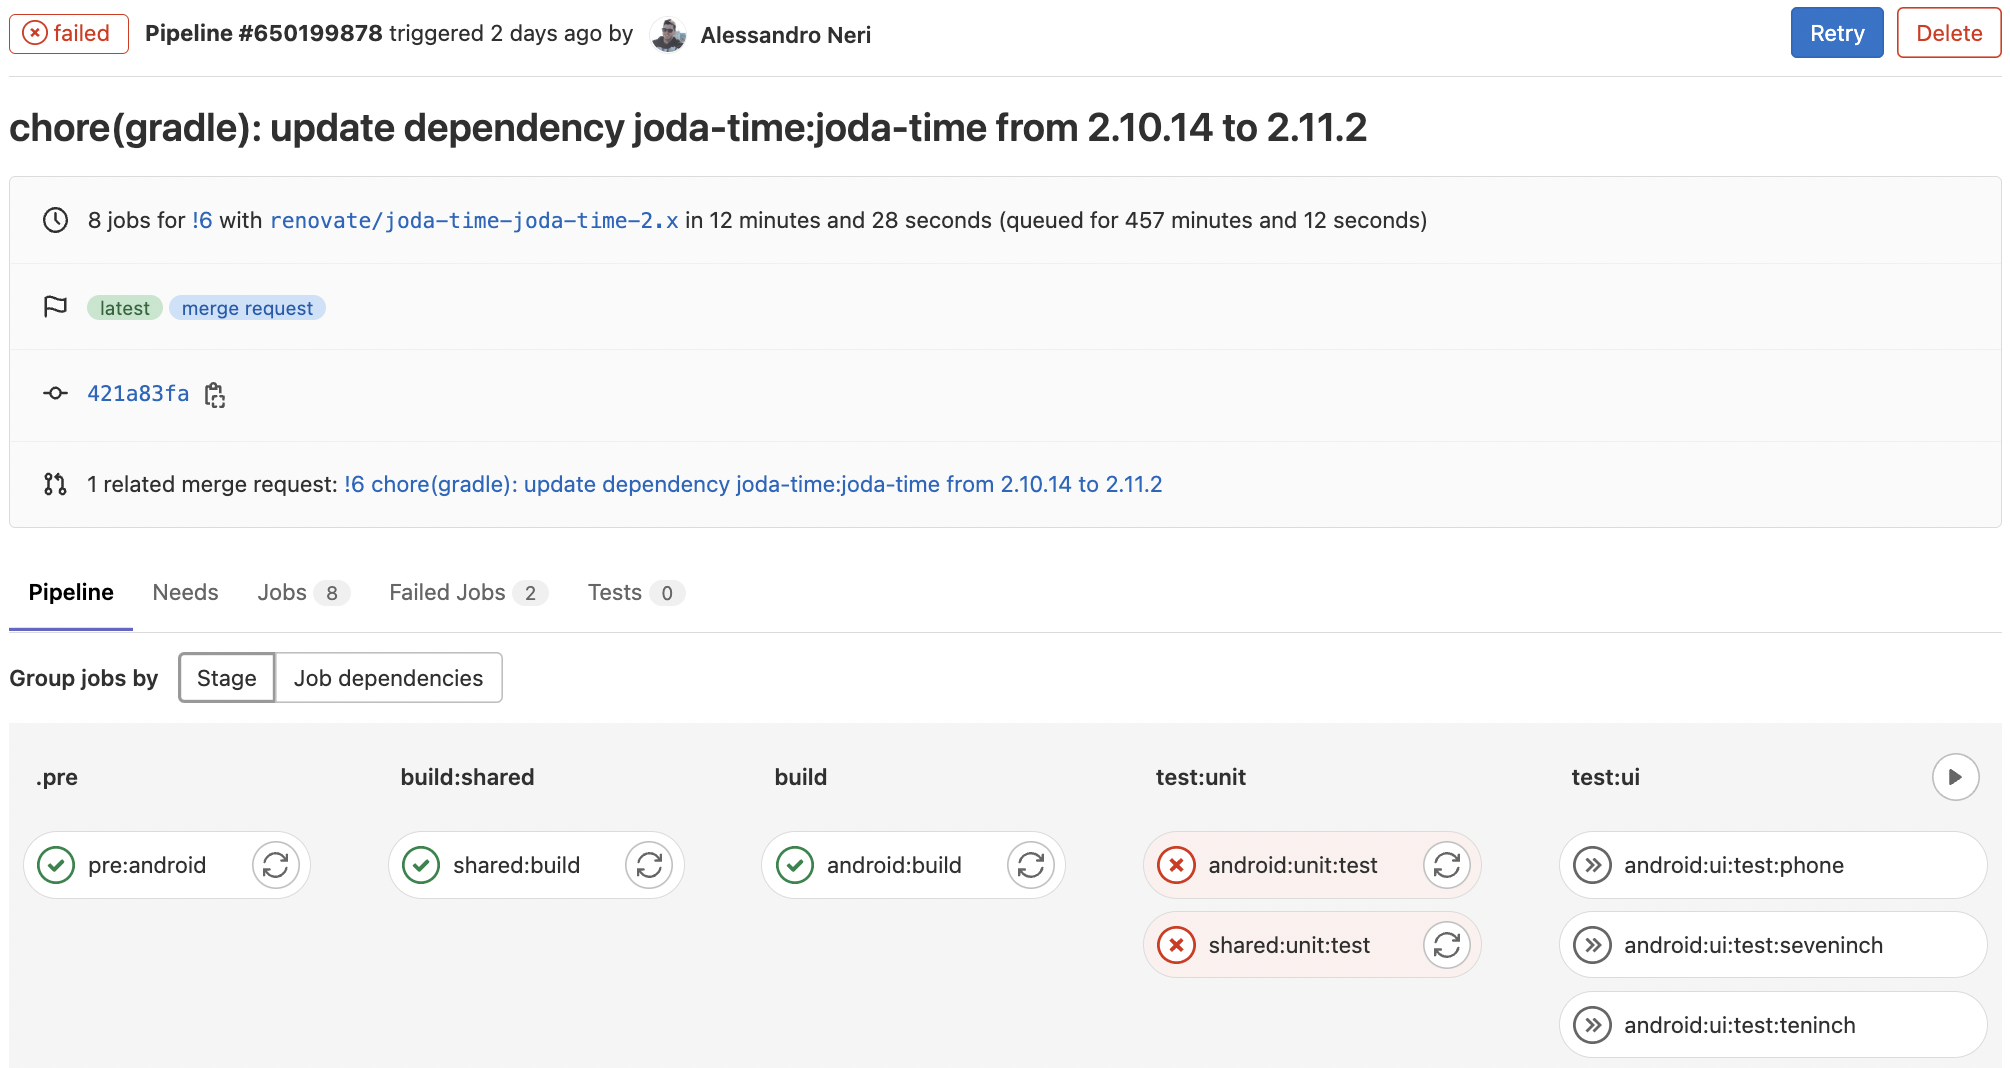
\includegraphics[width=1\textwidth]{img/Screenshot 2022-09-28 at 15.54.26.png}
    \caption{Schermata GitLab - Pipeline di aggiornamento delle dipendenze automatico fallita in fase di testing.}
    \label{mergerequestrenova}
\end{figure}

\section{Stabilizzazione e Rilascio}

La fase di stabilizzazione e rilascio della applicazione realizzata rispetta completamente quanto descritto nel capitolo \ref{ch:ch4}. Esistono dunque due fasi di stabilizzazione \textit{alpha} e \textit{beta} che corrispondono rispettivamente ai branch \textit{dev} e \textit{test}. La pubblicazione effettiva sullo store, equivalente all'ambiente di produzione, avviene in relazione alla modifica del branch \textit{main}.\\
Le figure coinvolte in fase di analisi dei requisiti e di modellazione del dominio, insieme ai Professori relatori di questo progetto di tesi, formano il gruppo dei tester:
\begin{multicols}{2}
    \begin{figure}[H]
\centering
    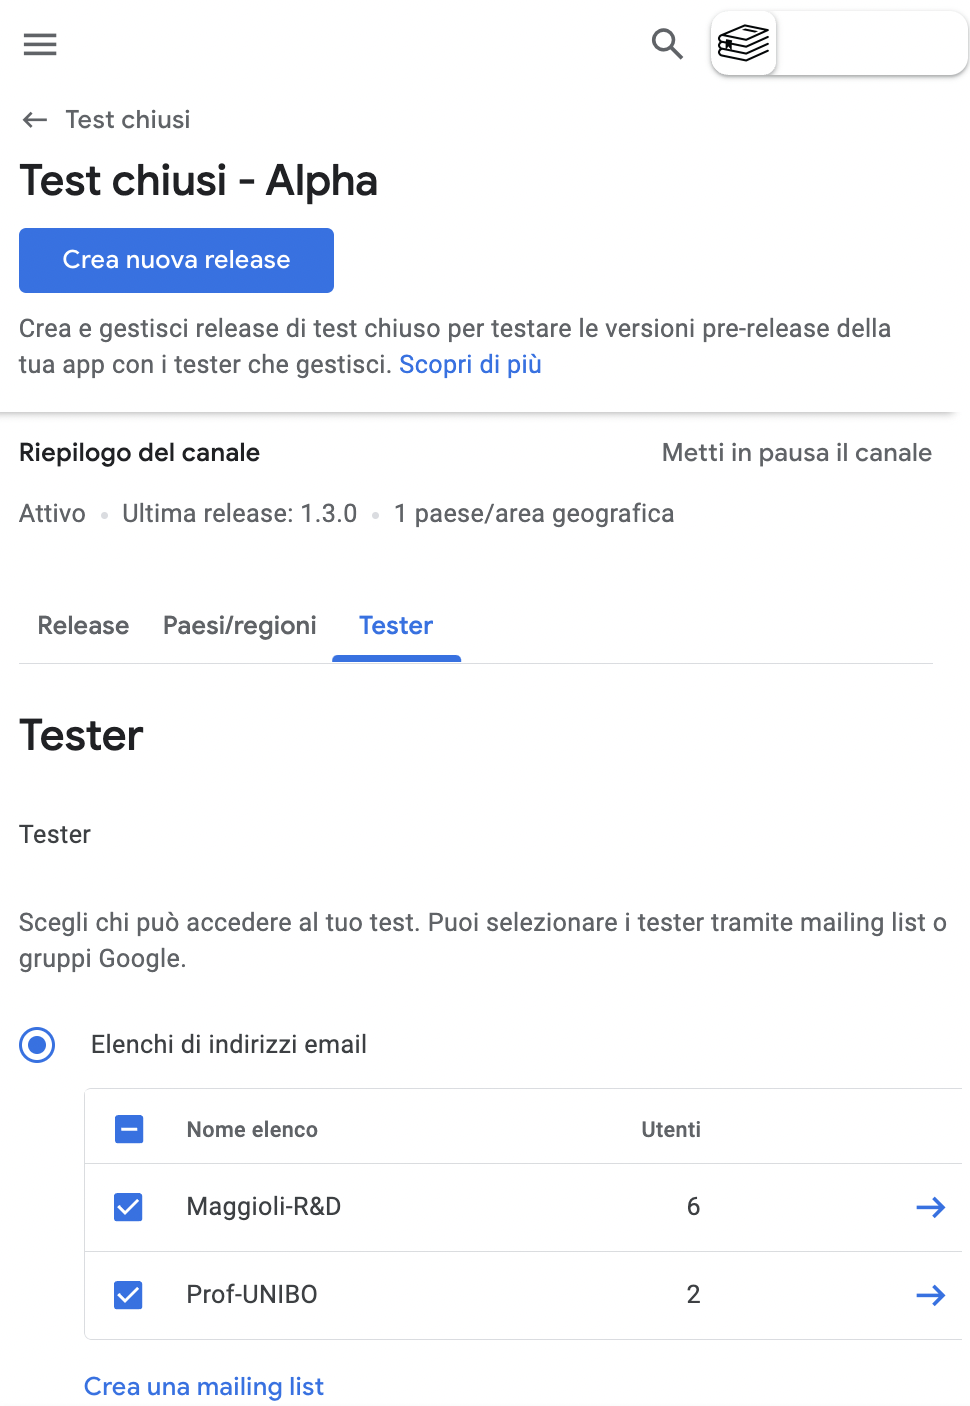
\includegraphics[width=0.45\textwidth]{img/Screenshot 2022-09-28 at 14.41.54.png}
    \caption{Mailing list di configurazione per il gruppo dei tester della applicazione Android (Google Play Console).}
    \label{mailinglisttester}
\end{figure}
\begin{figure}[H]
\centering
    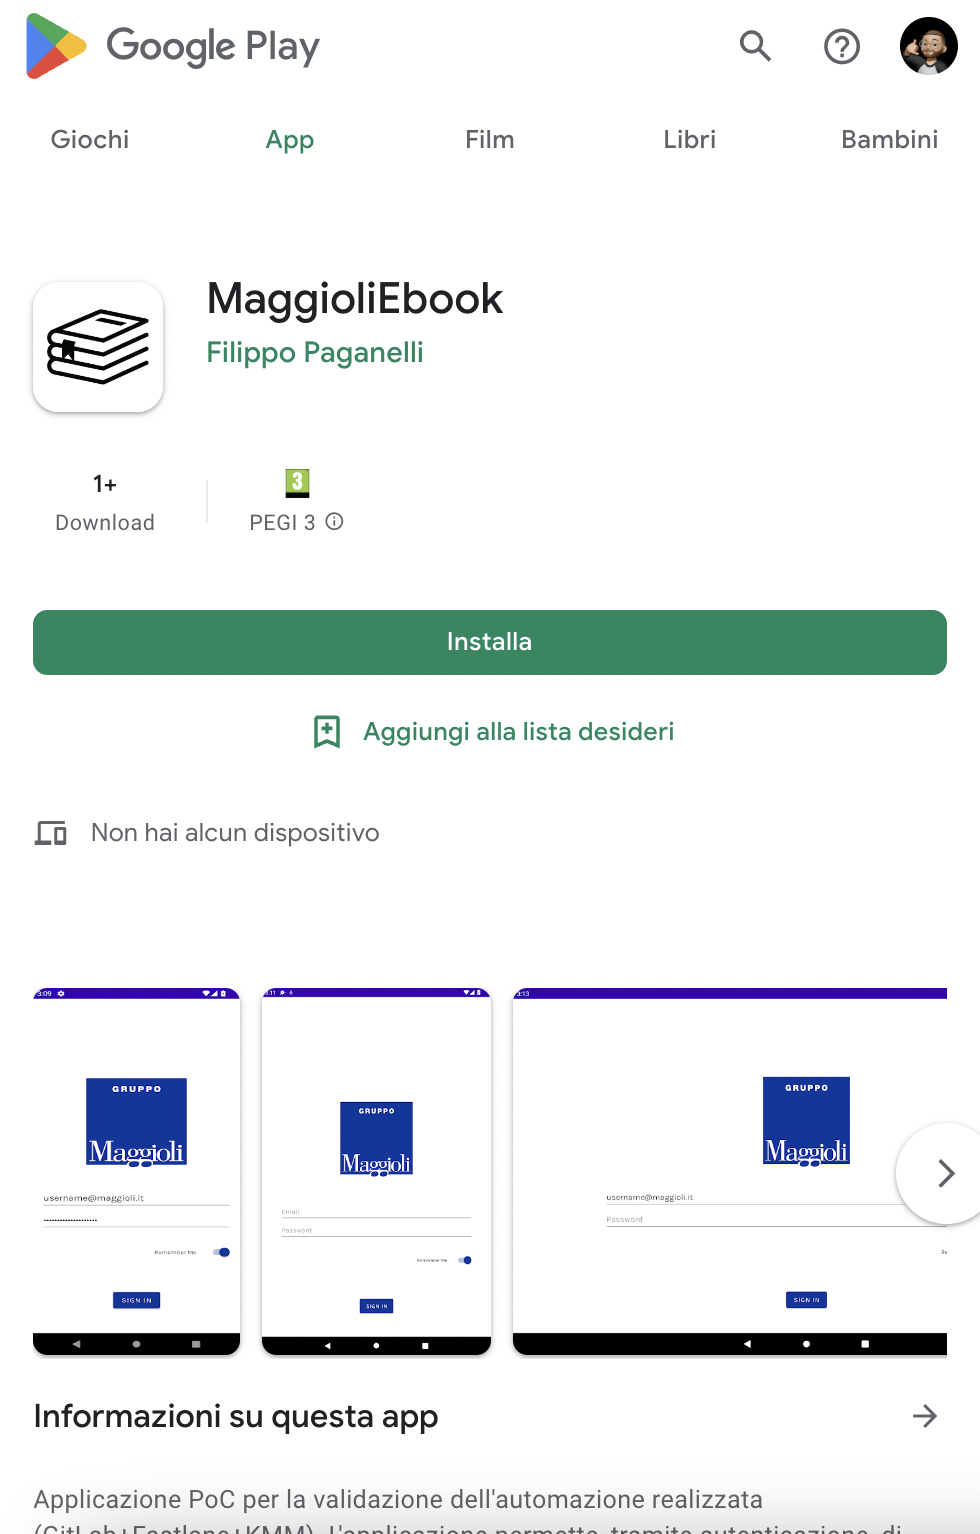
\includegraphics[width=0.45\textwidth]{img/Screenshot 2022-09-28 at 15.06.56.png}
    \caption{Pagina della applicazione Android pubblicata sullo store Google Play (disponibile solo per i tester presenti nella mailing list).}
    \label{playstoreapp}
\end{figure}
\end{multicols}

\newpage
\begin{multicols}{2}
\begin{figure}[H]
\centering
    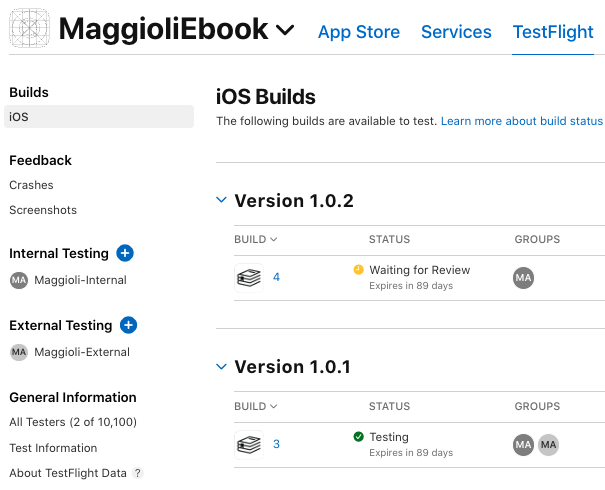
\includegraphics[width=0.55\textwidth]{img/Screenshot 2022-10-05 at 11.34.06.png}
    \caption{Mailing list di configurazione per il gruppo dei tester della applicazione iOS (App Store Connect).}
    \label{appstoreconnect}
\end{figure}
\begin{figure}[H]
\centering
    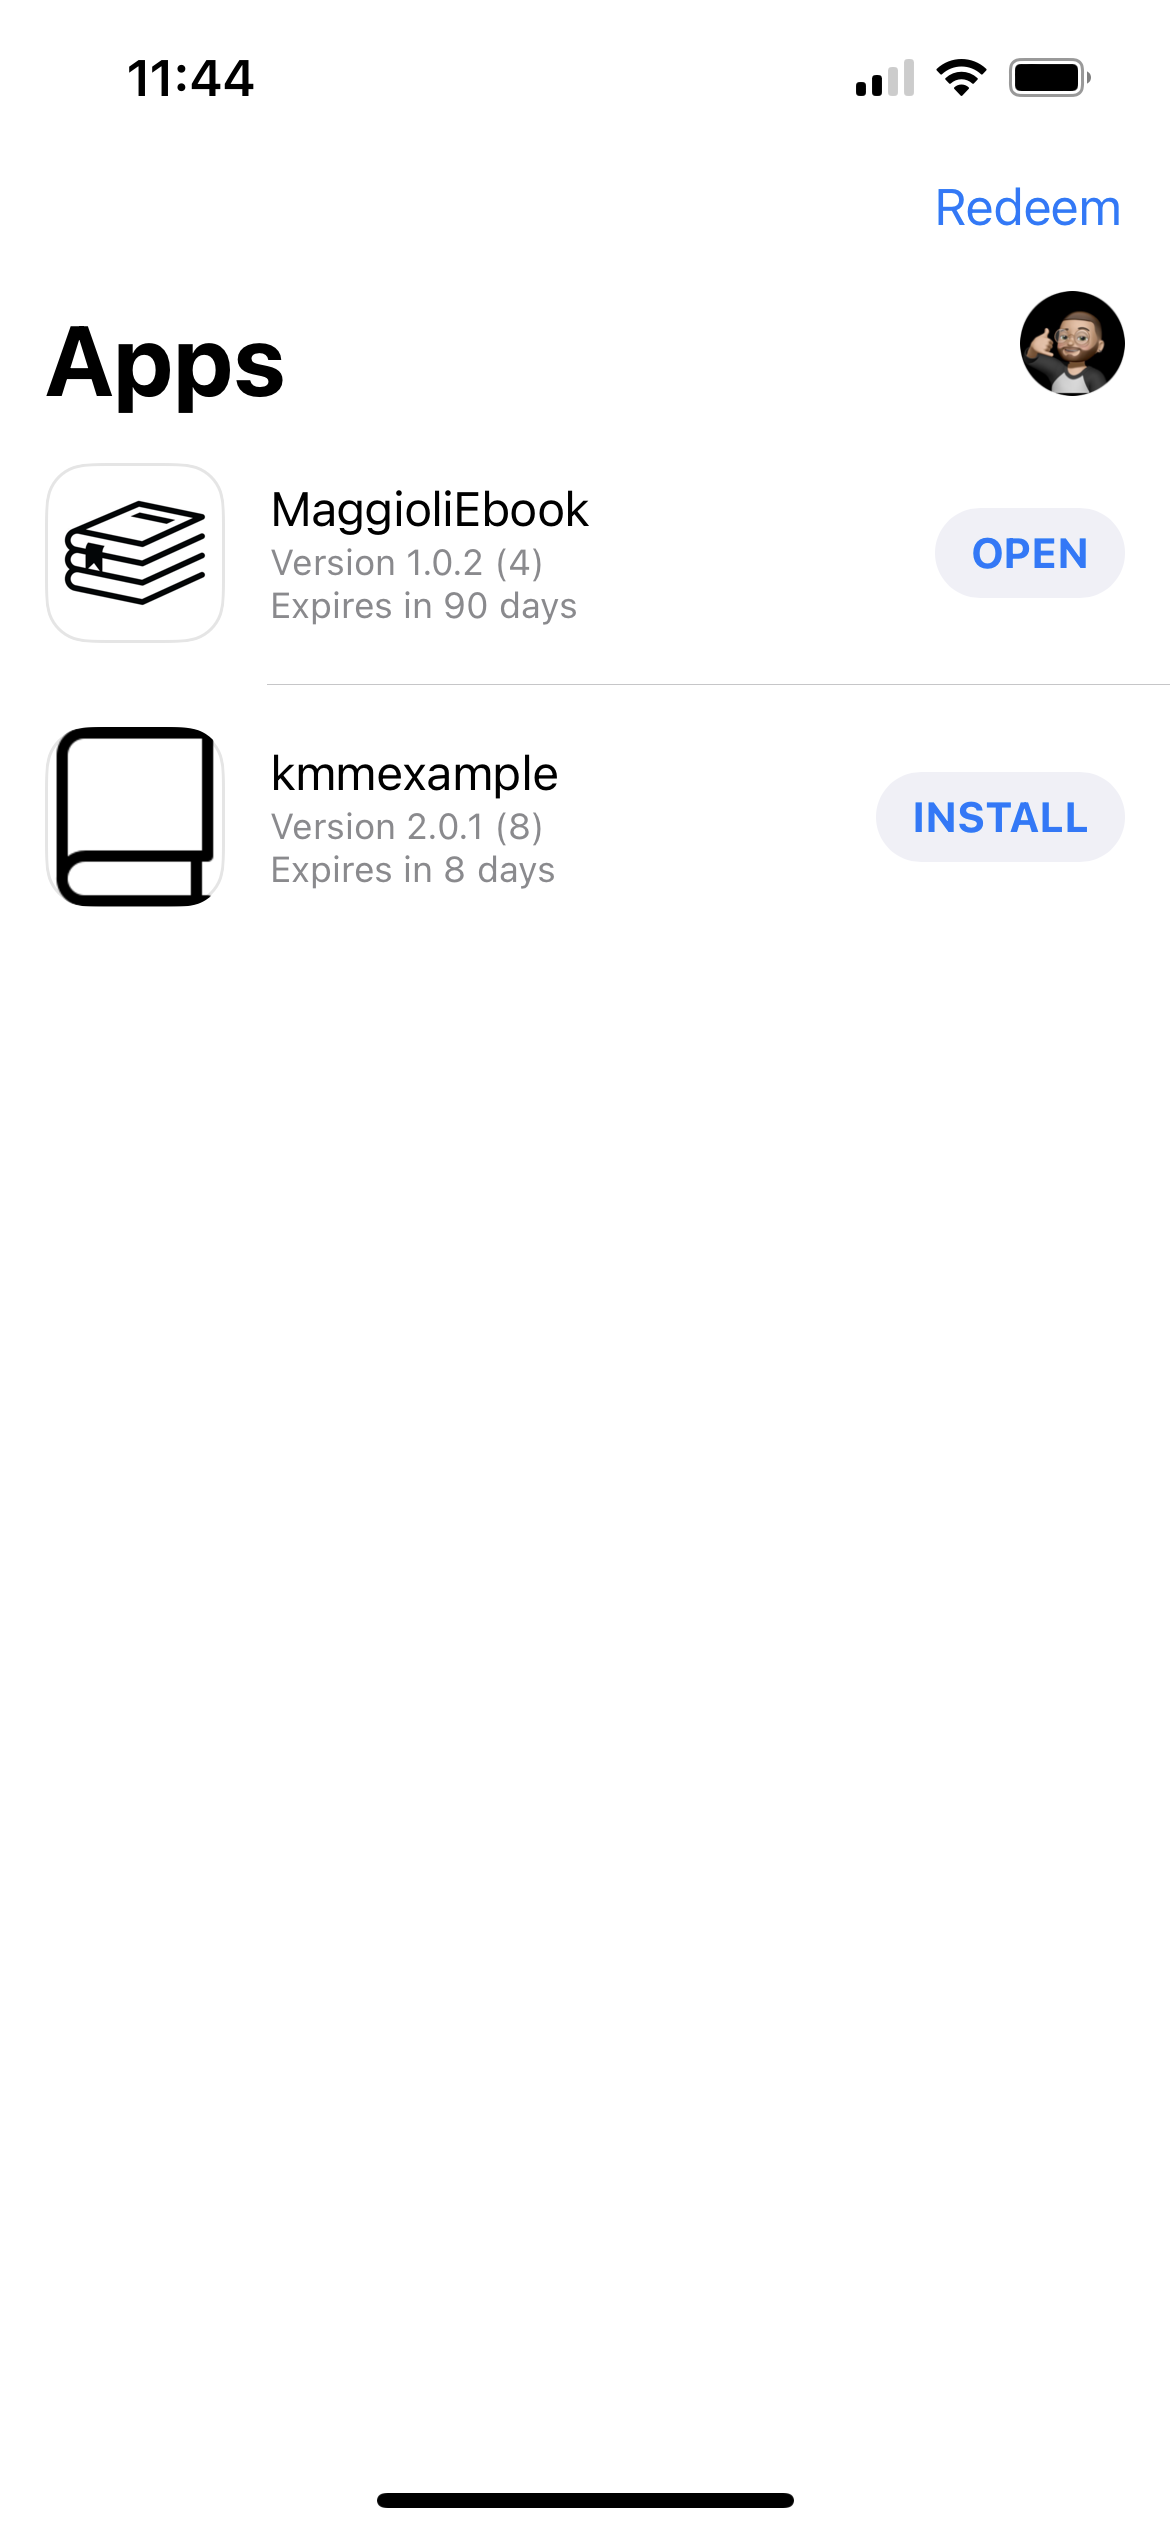
\includegraphics[width=0.35\textwidth]{img/IMG_1221.png}
    \caption{Screenshot applicazione Testflight (app scaricabile solo per i tester presenti nella mailing list).}
    \label{testflight}
\end{figure}
\end{multicols}

\subsection{Continuous Delivery}
Nelle seguenti schermate ottenute dalla piattaforma GitLab viene mostrato l'effettivo utilizzo delle tecniche di Continuous Delivery come descritto nel capitolo \ref{ch:ch4}. Le due pipeline per il rilascio alpha e beta terminate con successo (schermata \ref{pipelinesapp}) rappresentano un esempio completo del processo automatizzato, dalla compilazione al rilascio.

\begin{figure}[H]
\centering
    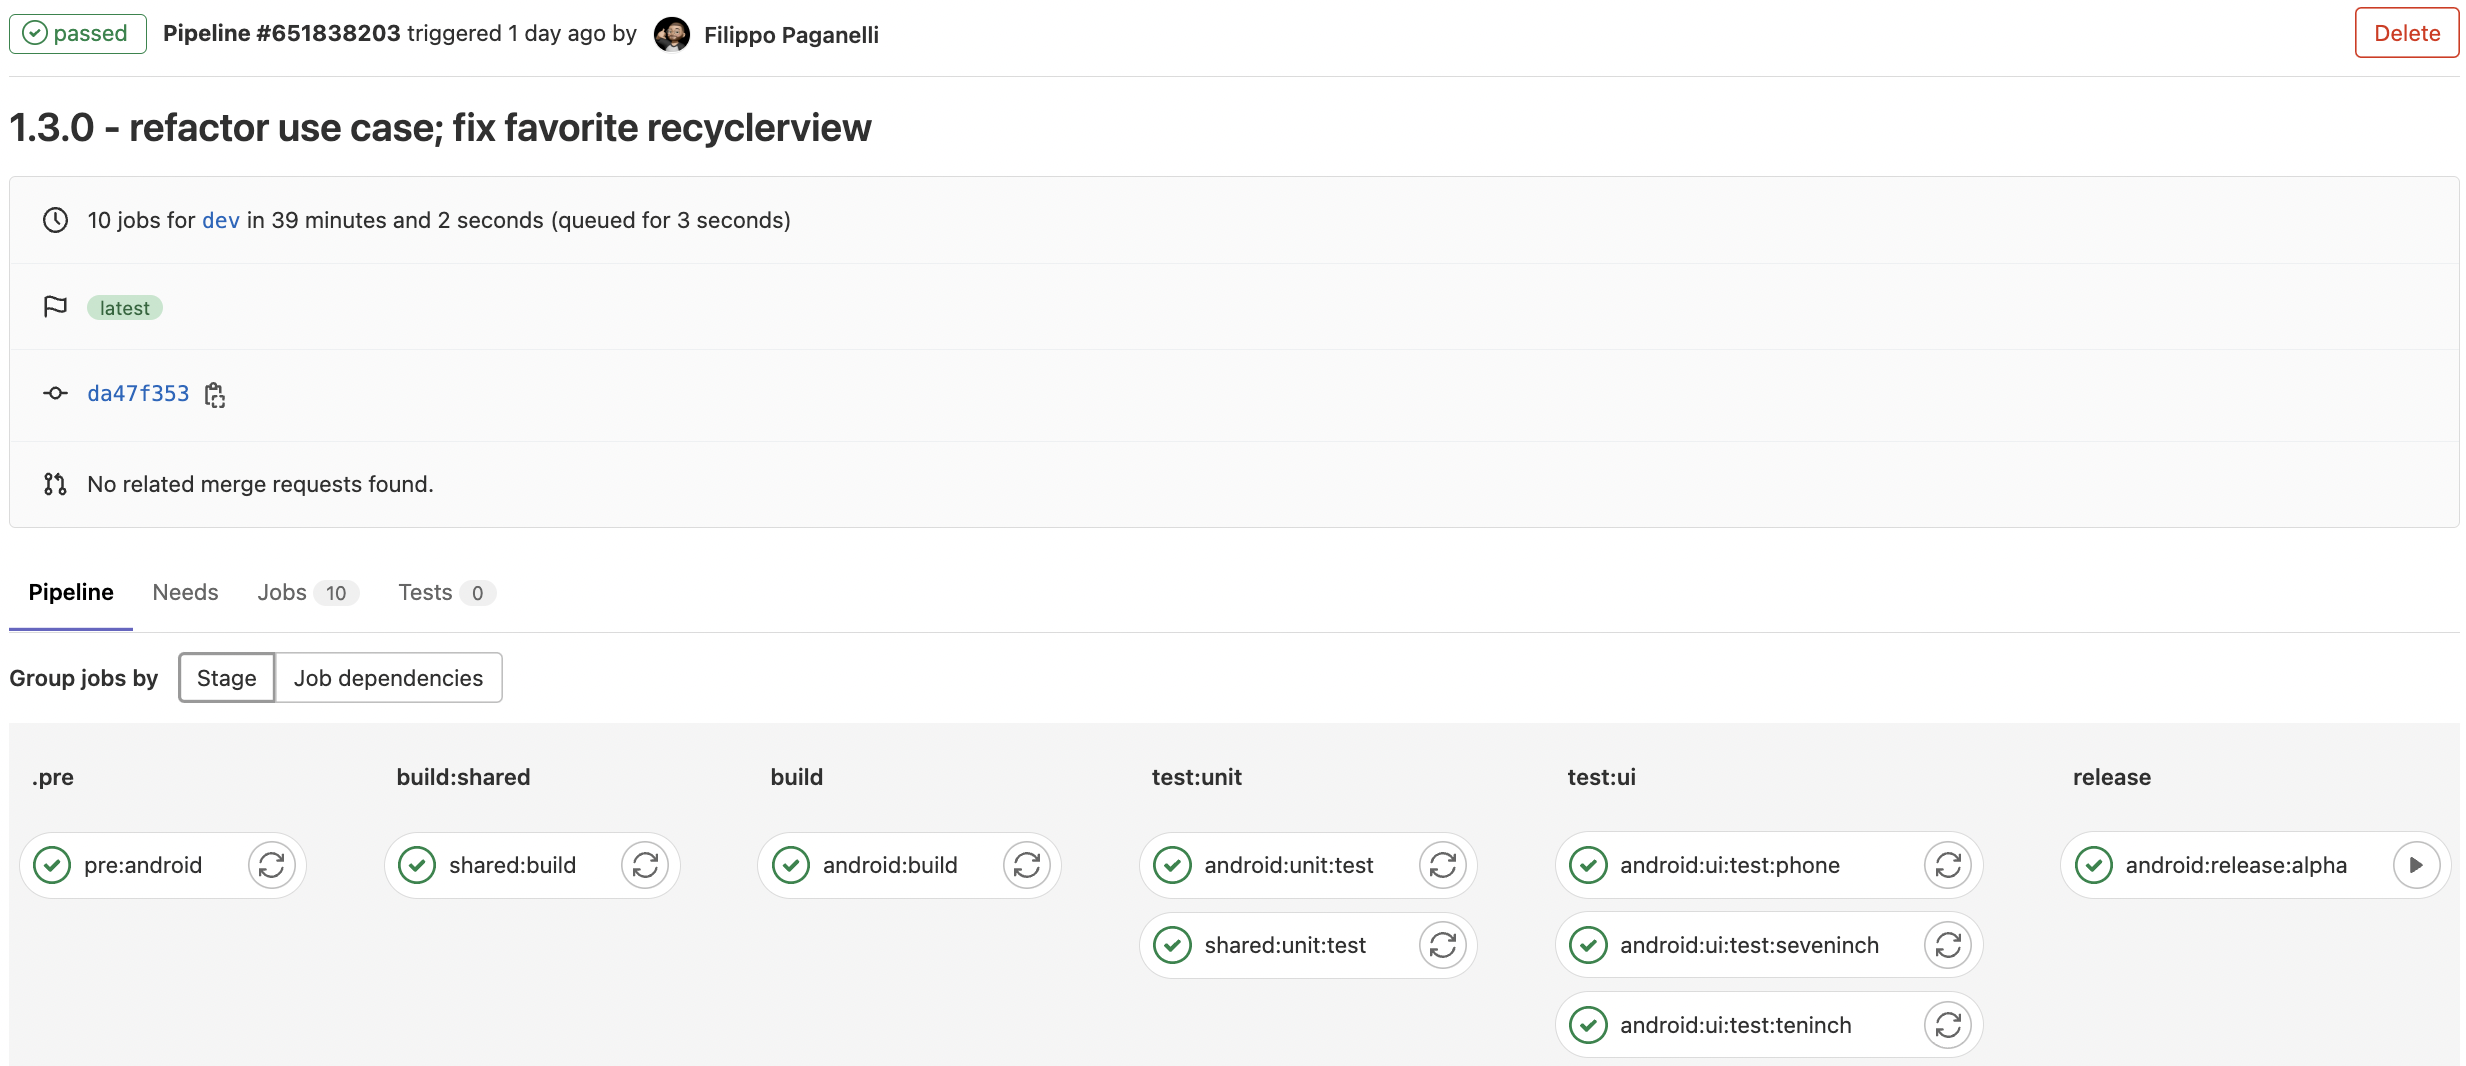
\includegraphics[width=1\textwidth]{img/Screenshot 2022-09-28 at 15.51.47.png}
    \caption{Schermata GitLab - Pipeline completa con rilascio Alpha.}
    \label{alpharelease}
\end{figure}

\begin{figure}[H]
\centering
    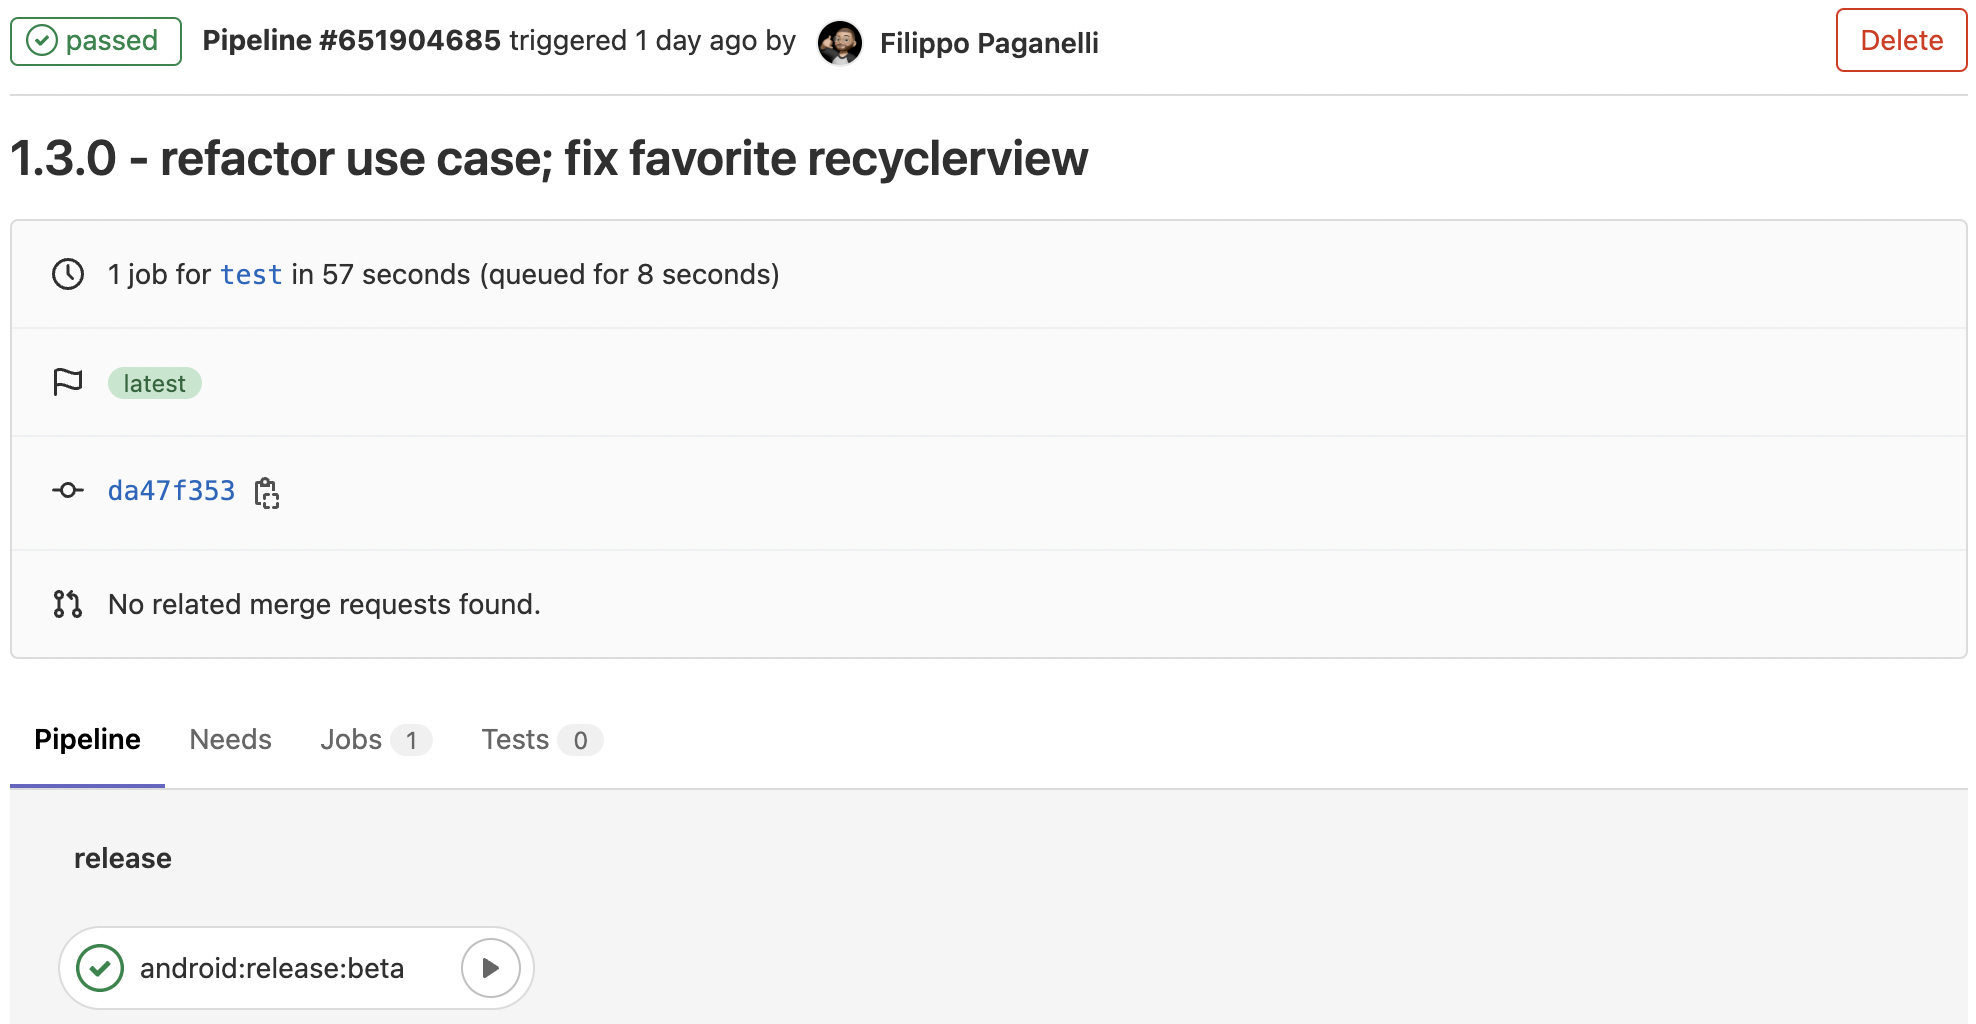
\includegraphics[width=1\textwidth]{img/Screenshot 2022-09-28 at 16.11.22.png}
    \caption{Schermata GitLab - Pipeline rilascio Beta.}
    \label{betarelease}
\end{figure}

\subsection{Continuous Inspection}
Le fasi di analisi del codice vengono eseguite in modo asincrono rispetto al flusso di sviluppo come descritto nel capitolo \ref{ch:ch4}. Le seguenti schermate mostrano l'utilizzo, con esisto positivo, delle tecniche di Continuous Inspection tramite l'esecuzione delle pipeline di analisi in GitLab e l'upload dei report sul servizio aziendale SonarQube:
\begin{figure}[H]
\centering
    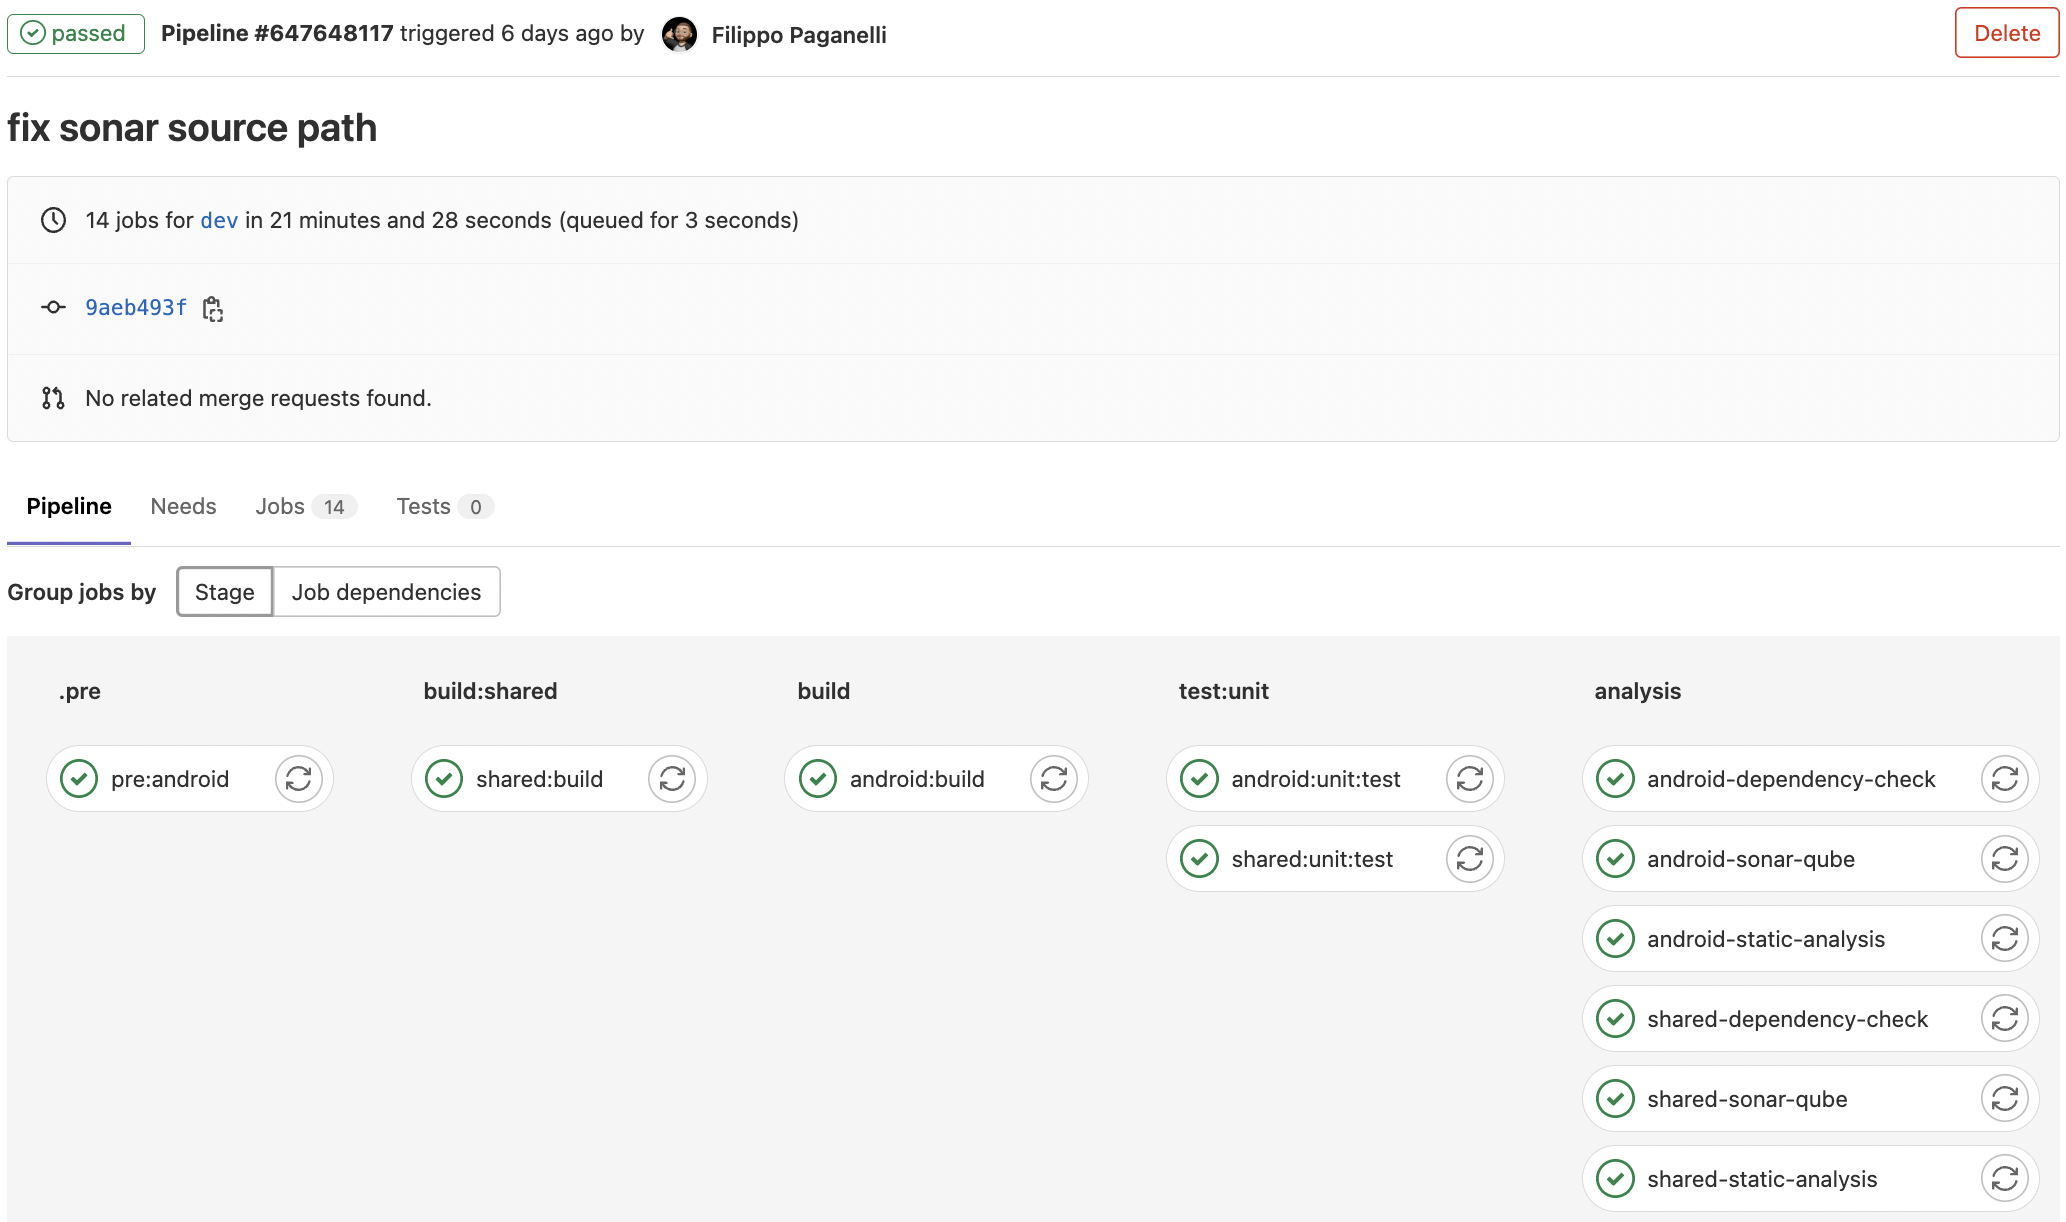
\includegraphics[width=1\textwidth]{img/Screenshot 2022-09-28 at 16.15.34.png}
    \caption{Schermata GitLab - Pipeline completa di analisi.}
    \label{fullpipeline}
\end{figure}

\begin{figure}[H]
\centering
    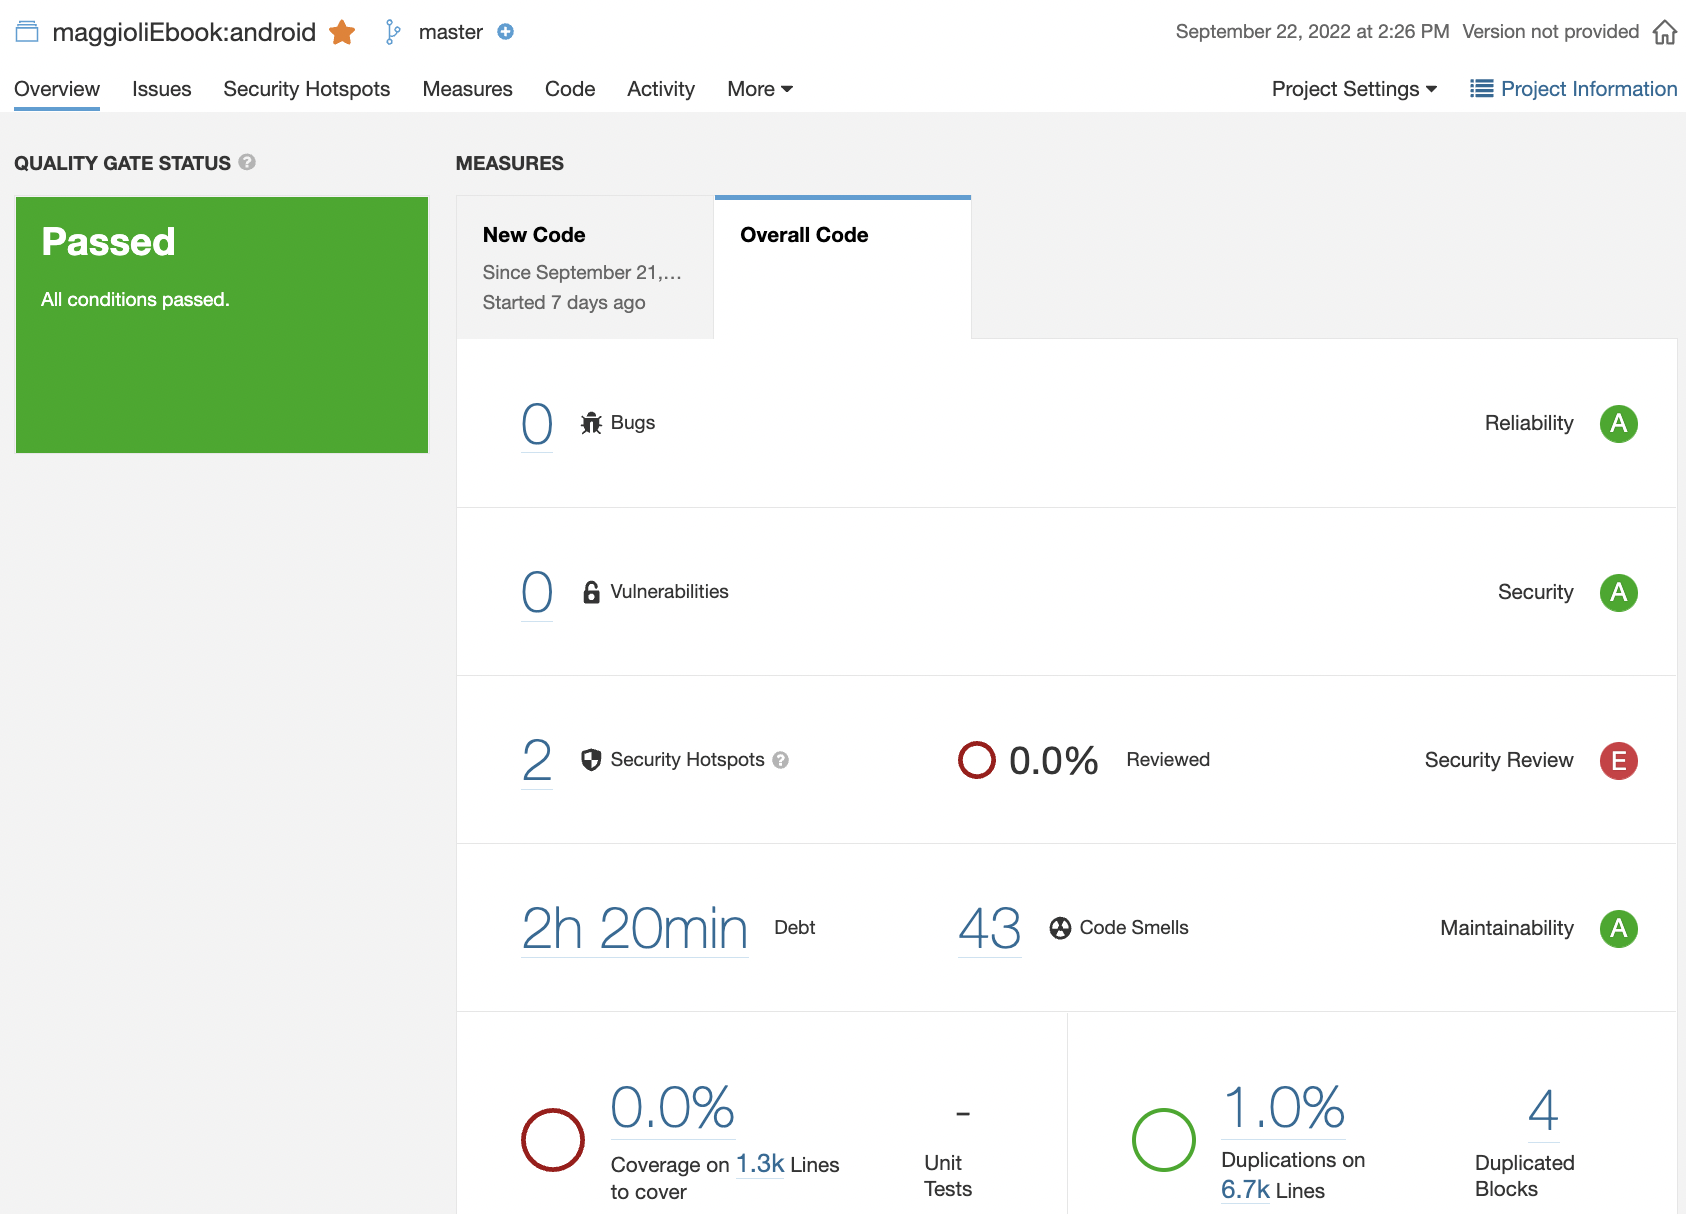
\includegraphics[width=1\textwidth]{img/Screenshot 2022-09-28 at 16.22.16.png}
    \caption{Schermata SonarQube - Overview analisi della applicazione Android.}
    \label{analisipipeline}
\end{figure}